% todo
% change notation for let, and modify the binding diagrams accordingly
% multiple let, especially in interpreters
% introduce some basic leftconn, rightconn exercises, in the style of the first part of the course
% font distinction for actual identifiers vs metasyntactic identifiers ranging over identifiers?  I think better not.
% symbol for operational behaviour of program would help
% motivate densem, not just tool for observational equivalences.
% talk about future, different effects, fine-grain call-by-value, call-by-push-value


\documentclass[runningheads,12pt]{llncs}
\usepackage{prooftree}
%% \message{<Paul Taylor's Proof Trees, 2 August 1996>}
%% Build proof tree for Natural Deduction, Sequent Calculus, etc.
%% WITH SHORTENING OF PROOF RULES!
%% Paul Taylor, begun 10 Oct 1989
%% *** THIS IS ONLY A PRELIMINARY VERSION AND THINGS MAY CHANGE! ***
%%
%% 2 Aug 1996: fixed \mscount and \proofdotnumber
%%
%%      \prooftree
%%              hyp1            produces:
%%              hyp2
%%              hyp3            hyp1    hyp2    hyp3
%%      \justifies              -------------------- rulename
%%              concl                   concl
%%      \thickness=0.08em
%%      \shiftright 2em
%%      \using
%%              rulename
%%      \endprooftree
%%
%% where the hypotheses may be similar structures or just formulae.
%%
%% To get a vertical string of dots instead of the proof rule, do
%%
%%      \prooftree                      which produces:
%%              [hyp]
%%      \using                                  [hyp]
%%              name                              .
%%      \proofdotseparation=1.2ex                 .name
%%      \proofdotnumber=4                         .
%%      \leadsto                                  .
%%              concl                           concl
%%      \endprooftree
%%
%% Within a prooftree, \[ and \] may be used instead of \prooftree and
%% \endprooftree; this is not permitted at the outer level because it
%% conflicts with LaTeX. Also,
%%      \Justifies
%% produces a double line. In LaTeX you can use \begin{prooftree} and
%% \end{prootree} at the outer level (however this will not work for the inner
%% levels, but in any case why would you want to be so verbose?).
%%
%% All of of the keywords except \prooftree and \endprooftree are optional
%% and may appear in any order. They may also be combined in \newcommand's
%% eg "\def\Cut{\using\sf cut\thickness.08em\justifies}" with the abbreviation
%% "\prooftree hyp1 hyp2 \Cut \concl \endprooftree". This is recommended and
%% some standard abbreviations will be found at the end of this file.
%%
%% \thickness specifies the breadth of the rule in any units, although
%% font-relative units such as "ex" or "em" are preferable.
%% It may optionally be followed by "=".
%% \proofrulebreadth=.08em or \setlength\proofrulebreadth{.08em} may also be
%% used either in place of \thickness or globally; the default is 0.04em.
%% \proofdotseparation and \proofdotnumber control the size of the
%% string of dots
%%
%% If proof trees and formulae are mixed, some explicit spacing is needed,
%% but don't put anything to the left of the left-most (or the right of
%% the right-most) hypothesis, or put it in braces, because this will cause
%% the indentation to be lost.
%%
%% By default the conclusion is centered wrt the left-most and right-most
%% immediate hypotheses (not their proofs); \shiftright or \shiftleft moves
%% it relative to this position. (Not sure about this specification or how
%% it should affect spreading of proof tree.)
%
% global assignments to dimensions seem to have the effect of stretching
% diagrams horizontally.
%
%%==========================================================================

\def\introrule{{\cal I}}\def\elimrule{{\cal E}}%%
\def\andintro{\using{\land}\introrule\justifies}%%
\def\impelim{\using{\Rightarrow}\elimrule\justifies}%%
\def\allintro{\using{\forall}\introrule\justifies}%%
\def\allelim{\using{\forall}\elimrule\justifies}%%
\def\falseelim{\using{\bot}\elimrule\justifies}%%
\def\existsintro{\using{\exists}\introrule\justifies}%%

%% #1 is meant to be 1 or 2 for the first or second formula
\def\andelim#1{\using{\land}#1\elimrule\justifies}%%
\def\orintro#1{\using{\lor}#1\introrule\justifies}%%

%% #1 is meant to be a label corresponding to the discharged hypothesis/es
\def\impintro#1{\using{\Rightarrow}\introrule_{#1}\justifies}%%
\def\orelim#1{\using{\lor}\elimrule_{#1}\justifies}%%
\def\existselim#1{\using{\exists}\elimrule_{#1}\justifies}

%%==========================================================================

\newdimen\proofrulebreadth \proofrulebreadth=.05em
\newdimen\proofdotseparation \proofdotseparation=1.25ex
\newdimen\proofrulebaseline \proofrulebaseline=2ex
\newcount\proofdotnumber \proofdotnumber=3
\let\then\relax
\def\hfi{\hskip0pt plus.0001fil}
\mathchardef\squigto="3A3B
%
% flag where we are
\newif\ifinsideprooftree\insideprooftreefalse
\newif\ifonleftofproofrule\onleftofproofrulefalse
\newif\ifproofdots\proofdotsfalse
\newif\ifdoubleproof\doubleprooffalse
\let\wereinproofbit\relax
%
% dimensions and boxes of bits
\newdimen\shortenproofleft
\newdimen\shortenproofright
\newdimen\proofbelowshift
\newbox\proofabove
\newbox\proofbelow
\newbox\proofrulename
%
% miscellaneous commands for setting values
\def\shiftproofbelow{\let\next\relax\afterassignment\setshiftproofbelow\dimen0 }
\def\shiftproofbelowneg{\def\next{\multiply\dimen0 by-1 }%
\afterassignment\setshiftproofbelow\dimen0 }
\def\setshiftproofbelow{\next\proofbelowshift=\dimen0 }
\def\setproofrulebreadth{\proofrulebreadth}

%=============================================================================
\def\prooftree{% NESTED ZERO (\ifonleftofproofrule)
%
% first find out whether we're at the left-hand end of a proof rule
\ifnum  \lastpenalty=1
\then   \unpenalty
\else   \onleftofproofrulefalse
\fi
%
% some space on left (except if we're on left, and no infinity for outermost)
\ifonleftofproofrule
\else   \ifinsideprooftree
        \then   \hskip.5em plus1fil
        \fi
\fi
%
% begin our proof tree environment
\bgroup% NESTED ONE (\proofbelow, \proofrulename, \proofabove,
%               \shortenproofleft, \shortenproofright, \proofrulebreadth)
\setbox\proofbelow=\hbox{}\setbox\proofrulename=\hbox{}%
\let\justifies\proofover\let\leadsto\proofoverdots\let\Justifies\proofoverdbl
\let\using\proofusing\let\[\prooftree
\ifinsideprooftree\let\]\endprooftree\fi
\proofdotsfalse\doubleprooffalse
\let\thickness\setproofrulebreadth
\let\shiftright\shiftproofbelow \let\shift\shiftproofbelow
\let\shiftleft\shiftproofbelowneg
\let\ifwasinsideprooftree\ifinsideprooftree
\insideprooftreetrue
%
% now begin to set the top of the rule (definitions local to it)
\setbox\proofabove=\hbox\bgroup$\displaystyle % NESTED TWO
\let\wereinproofbit\prooftree
%
% these local variables will be copied out:
\shortenproofleft=0pt \shortenproofright=0pt \proofbelowshift=0pt
%
% flags to enable inner proof tree to detect if on left:
\onleftofproofruletrue\penalty1
}

%=============================================================================
% end whatever box and copy crucial values out of it
\def\eproofbit{% NESTED TWO
%
% various hacks applicable to hypothesis list 
\ifx    \wereinproofbit\prooftree
\then   \ifcase \lastpenalty
        \then   \shortenproofright=0pt  % 0: some other object, no indentation
        \or     \unpenalty\hfil         % 1: empty hypotheses, just glue
        \or     \unpenalty\unskip       % 2: just had a tree, remove glue
        \else   \shortenproofright=0pt  % eh?
        \fi
\fi
%
% pass out crucial values from scope
\global\dimen0=\shortenproofleft
\global\dimen1=\shortenproofright
\global\dimen2=\proofrulebreadth
\global\dimen3=\proofbelowshift
\global\dimen4=\proofdotseparation
\global\count255=\proofdotnumber
%
% end the box
$\egroup  % NESTED ONE
%
% restore the values
\shortenproofleft=\dimen0
\shortenproofright=\dimen1
\proofrulebreadth=\dimen2
\proofbelowshift=\dimen3
\proofdotseparation=\dimen4
\proofdotnumber=\count255
}

%=============================================================================
\def\proofover{% NESTED TWO
\eproofbit % NESTED ONE
\setbox\proofbelow=\hbox\bgroup % NESTED TWO
\let\wereinproofbit\proofover
$\displaystyle
}%
%
%=============================================================================
\def\proofoverdbl{% NESTED TWO
\eproofbit % NESTED ONE
\doubleprooftrue
\setbox\proofbelow=\hbox\bgroup % NESTED TWO
\let\wereinproofbit\proofoverdbl
$\displaystyle
}%
%
%=============================================================================
\def\proofoverdots{% NESTED TWO
\eproofbit % NESTED ONE
\proofdotstrue
\setbox\proofbelow=\hbox\bgroup % NESTED TWO
\let\wereinproofbit\proofoverdots
$\displaystyle
}%
%
%=============================================================================
\def\proofusing{% NESTED TWO
\eproofbit % NESTED ONE
\setbox\proofrulename=\hbox\bgroup % NESTED TWO
\let\wereinproofbit\proofusing
\kern0.3em$
}

%=============================================================================
\def\endprooftree{% NESTED TWO
\eproofbit % NESTED ONE
% \dimen0 =     length of proof rule
% \dimen1 =     indentation of conclusion wrt rule
% \dimen2 =     new \shortenproofleft, ie indentation of conclusion
% \dimen3 =     new \shortenproofright, ie
%                space on right of conclusion to end of tree
% \dimen4 =     space on right of conclusion below rule
  \dimen5 =0pt% spread of hypotheses
% \dimen6, \dimen7 = height & depth of rule
%
% length of rule needed by proof above
\dimen0=\wd\proofabove \advance\dimen0-\shortenproofleft
\advance\dimen0-\shortenproofright
%
% amount of spare space below
\dimen1=.5\dimen0 \advance\dimen1-.5\wd\proofbelow
\dimen4=\dimen1
\advance\dimen1\proofbelowshift \advance\dimen4-\proofbelowshift
%
% conclusion sticks out to left of immediate hypotheses
\ifdim  \dimen1<0pt
\then   \advance\shortenproofleft\dimen1
        \advance\dimen0-\dimen1
        \dimen1=0pt
%       now it sticks out to left of tree!
        \ifdim  \shortenproofleft<0pt
        \then   \setbox\proofabove=\hbox{%
                        \kern-\shortenproofleft\unhbox\proofabove}%
                \shortenproofleft=0pt
        \fi
\fi
%
% and to the right
\ifdim  \dimen4<0pt
\then   \advance\shortenproofright\dimen4
        \advance\dimen0-\dimen4
        \dimen4=0pt
\fi
%
% make sure enough space for label
\ifdim  \shortenproofright<\wd\proofrulename
\then   \shortenproofright=\wd\proofrulename
\fi
%
% calculate new indentations
\dimen2=\shortenproofleft \advance\dimen2 by\dimen1
\dimen3=\shortenproofright\advance\dimen3 by\dimen4
%
% make the rule or dots, with name attached
\ifproofdots
\then
        \dimen6=\shortenproofleft \advance\dimen6 .5\dimen0
        \setbox1=\vbox to\proofdotseparation{\vss\hbox{$\cdot$}\vss}%
        \setbox0=\hbox{%
                \advance\dimen6-.5\wd1
                \kern\dimen6
                $\vcenter to\proofdotnumber\proofdotseparation
                        {\leaders\box1\vfill}$%
                \unhbox\proofrulename}%
\else   \dimen6=\fontdimen22\the\textfont2 % height of maths axis
        \dimen7=\dimen6
        \advance\dimen6by.5\proofrulebreadth
        \advance\dimen7by-.5\proofrulebreadth
        \setbox0=\hbox{%
                \kern\shortenproofleft
                \ifdoubleproof
                \then   \hbox to\dimen0{%
                        $\mathsurround0pt\mathord=\mkern-6mu%
                        \cleaders\hbox{$\mkern-2mu=\mkern-2mu$}\hfill
                        \mkern-6mu\mathord=$}%
                \else   \vrule height\dimen6 depth-\dimen7 width\dimen0
                \fi
                \unhbox\proofrulename}%
        \ht0=\dimen6 \dp0=-\dimen7
\fi
%
% set up to centre outermost tree only
\let\doll\relax
\ifwasinsideprooftree
\then   \let\VBOX\vbox
\else   \ifmmode\else$\let\doll=$\fi
        \let\VBOX\vcenter
\fi
% this \vbox or \vcenter is the actual output:
\VBOX   {\baselineskip\proofrulebaseline \lineskip.2ex
        \expandafter\lineskiplimit\ifproofdots0ex\else-0.6ex\fi
        \hbox   spread\dimen5   {\hfi\unhbox\proofabove\hfi}%
        \hbox{\box0}%
        \hbox   {\kern\dimen2 \box\proofbelow}}\doll%
%
% pass new indentations out of scope
\global\dimen2=\dimen2
\global\dimen3=\dimen3
\egroup % NESTED ZERO
\ifonleftofproofrule
\then   \shortenproofleft=\dimen2
\fi
\shortenproofright=\dimen3
%
% some space on right and flag we've just made a tree
\onleftofproofrulefalse
\ifinsideprooftree
\then   \hskip.5em plus 1fil \penalty2
\fi
}

\endinput

%==========================================================================
% IDEAS
% 1.    Specification of \shiftright and how to spread trees.
% 2.    Spacing command \m which causes 1em+1fil spacing, over-riding
%       exisiting space on sides of trees and not affecting the
%       detection of being on the left or right.
% 3.    Hack using \@currenvir to detect LaTeX environment; have to
%       use \aftergroup to pass \shortenproofleft/right out.
% 4.    (Pie in the sky) detect how much trees can be "tucked in"
% 5.    Discharged hypotheses (diagonal lines).

Date: Tue, 19 May 1998 16:45:32 +0100
From: Simon Gay <simon@dcs.rhbnc.ac.uk>

I've got another problem when combining
your packages with elsart.cls. The code

\documentclass{elsart}
\message{<Paul Taylor's Proof Trees, 2 August 1996>}
%% Build proof tree for Natural Deduction, Sequent Calculus, etc.
%% WITH SHORTENING OF PROOF RULES!
%% Paul Taylor, begun 10 Oct 1989
%% *** THIS IS ONLY A PRELIMINARY VERSION AND THINGS MAY CHANGE! ***
%%
%% 2 Aug 1996: fixed \mscount and \proofdotnumber
%%
%%      \prooftree
%%              hyp1            produces:
%%              hyp2
%%              hyp3            hyp1    hyp2    hyp3
%%      \justifies              -------------------- rulename
%%              concl                   concl
%%      \thickness=0.08em
%%      \shiftright 2em
%%      \using
%%              rulename
%%      \endprooftree
%%
%% where the hypotheses may be similar structures or just formulae.
%%
%% To get a vertical string of dots instead of the proof rule, do
%%
%%      \prooftree                      which produces:
%%              [hyp]
%%      \using                                  [hyp]
%%              name                              .
%%      \proofdotseparation=1.2ex                 .name
%%      \proofdotnumber=4                         .
%%      \leadsto                                  .
%%              concl                           concl
%%      \endprooftree
%%
%% Within a prooftree, \[ and \] may be used instead of \prooftree and
%% \endprooftree; this is not permitted at the outer level because it
%% conflicts with LaTeX. Also,
%%      \Justifies
%% produces a double line. In LaTeX you can use \begin{prooftree} and
%% \end{prootree} at the outer level (however this will not work for the inner
%% levels, but in any case why would you want to be so verbose?).
%%
%% All of of the keywords except \prooftree and \endprooftree are optional
%% and may appear in any order. They may also be combined in \newcommand's
%% eg "\def\Cut{\using\sf cut\thickness.08em\justifies}" with the abbreviation
%% "\prooftree hyp1 hyp2 \Cut \concl \endprooftree". This is recommended and
%% some standard abbreviations will be found at the end of this file.
%%
%% \thickness specifies the breadth of the rule in any units, although
%% font-relative units such as "ex" or "em" are preferable.
%% It may optionally be followed by "=".
%% \proofrulebreadth=.08em or \setlength\proofrulebreadth{.08em} may also be
%% used either in place of \thickness or globally; the default is 0.04em.
%% \proofdotseparation and \proofdotnumber control the size of the
%% string of dots
%%
%% If proof trees and formulae are mixed, some explicit spacing is needed,
%% but don't put anything to the left of the left-most (or the right of
%% the right-most) hypothesis, or put it in braces, because this will cause
%% the indentation to be lost.
%%
%% By default the conclusion is centered wrt the left-most and right-most
%% immediate hypotheses (not their proofs); \shiftright or \shiftleft moves
%% it relative to this position. (Not sure about this specification or how
%% it should affect spreading of proof tree.)
%
% global assignments to dimensions seem to have the effect of stretching
% diagrams horizontally.
%
%%==========================================================================

\def\introrule{{\cal I}}\def\elimrule{{\cal E}}%%
\def\andintro{\using{\land}\introrule\justifies}%%
\def\impelim{\using{\Rightarrow}\elimrule\justifies}%%
\def\allintro{\using{\forall}\introrule\justifies}%%
\def\allelim{\using{\forall}\elimrule\justifies}%%
\def\falseelim{\using{\bot}\elimrule\justifies}%%
\def\existsintro{\using{\exists}\introrule\justifies}%%

%% #1 is meant to be 1 or 2 for the first or second formula
\def\andelim#1{\using{\land}#1\elimrule\justifies}%%
\def\orintro#1{\using{\lor}#1\introrule\justifies}%%

%% #1 is meant to be a label corresponding to the discharged hypothesis/es
\def\impintro#1{\using{\Rightarrow}\introrule_{#1}\justifies}%%
\def\orelim#1{\using{\lor}\elimrule_{#1}\justifies}%%
\def\existselim#1{\using{\exists}\elimrule_{#1}\justifies}

%%==========================================================================

\newdimen\proofrulebreadth \proofrulebreadth=.05em
\newdimen\proofdotseparation \proofdotseparation=1.25ex
\newdimen\proofrulebaseline \proofrulebaseline=2ex
\newcount\proofdotnumber \proofdotnumber=3
\let\then\relax
\def\hfi{\hskip0pt plus.0001fil}
\mathchardef\squigto="3A3B
%
% flag where we are
\newif\ifinsideprooftree\insideprooftreefalse
\newif\ifonleftofproofrule\onleftofproofrulefalse
\newif\ifproofdots\proofdotsfalse
\newif\ifdoubleproof\doubleprooffalse
\let\wereinproofbit\relax
%
% dimensions and boxes of bits
\newdimen\shortenproofleft
\newdimen\shortenproofright
\newdimen\proofbelowshift
\newbox\proofabove
\newbox\proofbelow
\newbox\proofrulename
%
% miscellaneous commands for setting values
\def\shiftproofbelow{\let\next\relax\afterassignment\setshiftproofbelow\dimen0 }
\def\shiftproofbelowneg{\def\next{\multiply\dimen0 by-1 }%
\afterassignment\setshiftproofbelow\dimen0 }
\def\setshiftproofbelow{\next\proofbelowshift=\dimen0 }
\def\setproofrulebreadth{\proofrulebreadth}

%=============================================================================
\def\prooftree{% NESTED ZERO (\ifonleftofproofrule)
%
% first find out whether we're at the left-hand end of a proof rule
\ifnum  \lastpenalty=1
\then   \unpenalty
\else   \onleftofproofrulefalse
\fi
%
% some space on left (except if we're on left, and no infinity for outermost)
\ifonleftofproofrule
\else   \ifinsideprooftree
        \then   \hskip.5em plus1fil
        \fi
\fi
%
% begin our proof tree environment
\bgroup% NESTED ONE (\proofbelow, \proofrulename, \proofabove,
%               \shortenproofleft, \shortenproofright, \proofrulebreadth)
\setbox\proofbelow=\hbox{}\setbox\proofrulename=\hbox{}%
\let\justifies\proofover\let\leadsto\proofoverdots\let\Justifies\proofoverdbl
\let\using\proofusing\let\[\prooftree
\ifinsideprooftree\let\]\endprooftree\fi
\proofdotsfalse\doubleprooffalse
\let\thickness\setproofrulebreadth
\let\shiftright\shiftproofbelow \let\shift\shiftproofbelow
\let\shiftleft\shiftproofbelowneg
\let\ifwasinsideprooftree\ifinsideprooftree
\insideprooftreetrue
%
% now begin to set the top of the rule (definitions local to it)
\setbox\proofabove=\hbox\bgroup$\displaystyle % NESTED TWO
\let\wereinproofbit\prooftree
%
% these local variables will be copied out:
\shortenproofleft=0pt \shortenproofright=0pt \proofbelowshift=0pt
%
% flags to enable inner proof tree to detect if on left:
\onleftofproofruletrue\penalty1
}

%=============================================================================
% end whatever box and copy crucial values out of it
\def\eproofbit{% NESTED TWO
%
% various hacks applicable to hypothesis list 
\ifx    \wereinproofbit\prooftree
\then   \ifcase \lastpenalty
        \then   \shortenproofright=0pt  % 0: some other object, no indentation
        \or     \unpenalty\hfil         % 1: empty hypotheses, just glue
        \or     \unpenalty\unskip       % 2: just had a tree, remove glue
        \else   \shortenproofright=0pt  % eh?
        \fi
\fi
%
% pass out crucial values from scope
\global\dimen0=\shortenproofleft
\global\dimen1=\shortenproofright
\global\dimen2=\proofrulebreadth
\global\dimen3=\proofbelowshift
\global\dimen4=\proofdotseparation
\global\count255=\proofdotnumber
%
% end the box
$\egroup  % NESTED ONE
%
% restore the values
\shortenproofleft=\dimen0
\shortenproofright=\dimen1
\proofrulebreadth=\dimen2
\proofbelowshift=\dimen3
\proofdotseparation=\dimen4
\proofdotnumber=\count255
}

%=============================================================================
\def\proofover{% NESTED TWO
\eproofbit % NESTED ONE
\setbox\proofbelow=\hbox\bgroup % NESTED TWO
\let\wereinproofbit\proofover
$\displaystyle
}%
%
%=============================================================================
\def\proofoverdbl{% NESTED TWO
\eproofbit % NESTED ONE
\doubleprooftrue
\setbox\proofbelow=\hbox\bgroup % NESTED TWO
\let\wereinproofbit\proofoverdbl
$\displaystyle
}%
%
%=============================================================================
\def\proofoverdots{% NESTED TWO
\eproofbit % NESTED ONE
\proofdotstrue
\setbox\proofbelow=\hbox\bgroup % NESTED TWO
\let\wereinproofbit\proofoverdots
$\displaystyle
}%
%
%=============================================================================
\def\proofusing{% NESTED TWO
\eproofbit % NESTED ONE
\setbox\proofrulename=\hbox\bgroup % NESTED TWO
\let\wereinproofbit\proofusing
\kern0.3em$
}

%=============================================================================
\def\endprooftree{% NESTED TWO
\eproofbit % NESTED ONE
% \dimen0 =     length of proof rule
% \dimen1 =     indentation of conclusion wrt rule
% \dimen2 =     new \shortenproofleft, ie indentation of conclusion
% \dimen3 =     new \shortenproofright, ie
%                space on right of conclusion to end of tree
% \dimen4 =     space on right of conclusion below rule
  \dimen5 =0pt% spread of hypotheses
% \dimen6, \dimen7 = height & depth of rule
%
% length of rule needed by proof above
\dimen0=\wd\proofabove \advance\dimen0-\shortenproofleft
\advance\dimen0-\shortenproofright
%
% amount of spare space below
\dimen1=.5\dimen0 \advance\dimen1-.5\wd\proofbelow
\dimen4=\dimen1
\advance\dimen1\proofbelowshift \advance\dimen4-\proofbelowshift
%
% conclusion sticks out to left of immediate hypotheses
\ifdim  \dimen1<0pt
\then   \advance\shortenproofleft\dimen1
        \advance\dimen0-\dimen1
        \dimen1=0pt
%       now it sticks out to left of tree!
        \ifdim  \shortenproofleft<0pt
        \then   \setbox\proofabove=\hbox{%
                        \kern-\shortenproofleft\unhbox\proofabove}%
                \shortenproofleft=0pt
        \fi
\fi
%
% and to the right
\ifdim  \dimen4<0pt
\then   \advance\shortenproofright\dimen4
        \advance\dimen0-\dimen4
        \dimen4=0pt
\fi
%
% make sure enough space for label
\ifdim  \shortenproofright<\wd\proofrulename
\then   \shortenproofright=\wd\proofrulename
\fi
%
% calculate new indentations
\dimen2=\shortenproofleft \advance\dimen2 by\dimen1
\dimen3=\shortenproofright\advance\dimen3 by\dimen4
%
% make the rule or dots, with name attached
\ifproofdots
\then
        \dimen6=\shortenproofleft \advance\dimen6 .5\dimen0
        \setbox1=\vbox to\proofdotseparation{\vss\hbox{$\cdot$}\vss}%
        \setbox0=\hbox{%
                \advance\dimen6-.5\wd1
                \kern\dimen6
                $\vcenter to\proofdotnumber\proofdotseparation
                        {\leaders\box1\vfill}$%
                \unhbox\proofrulename}%
\else   \dimen6=\fontdimen22\the\textfont2 % height of maths axis
        \dimen7=\dimen6
        \advance\dimen6by.5\proofrulebreadth
        \advance\dimen7by-.5\proofrulebreadth
        \setbox0=\hbox{%
                \kern\shortenproofleft
                \ifdoubleproof
                \then   \hbox to\dimen0{%
                        $\mathsurround0pt\mathord=\mkern-6mu%
                        \cleaders\hbox{$\mkern-2mu=\mkern-2mu$}\hfill
                        \mkern-6mu\mathord=$}%
                \else   \vrule height\dimen6 depth-\dimen7 width\dimen0
                \fi
                \unhbox\proofrulename}%
        \ht0=\dimen6 \dp0=-\dimen7
\fi
%
% set up to centre outermost tree only
\let\doll\relax
\ifwasinsideprooftree
\then   \let\VBOX\vbox
\else   \ifmmode\else$\let\doll=$\fi
        \let\VBOX\vcenter
\fi
% this \vbox or \vcenter is the actual output:
\VBOX   {\baselineskip\proofrulebaseline \lineskip.2ex
        \expandafter\lineskiplimit\ifproofdots0ex\else-0.6ex\fi
        \hbox   spread\dimen5   {\hfi\unhbox\proofabove\hfi}%
        \hbox{\box0}%
        \hbox   {\kern\dimen2 \box\proofbelow}}\doll%
%
% pass new indentations out of scope
\global\dimen2=\dimen2
\global\dimen3=\dimen3
\egroup % NESTED ZERO
\ifonleftofproofrule
\then   \shortenproofleft=\dimen2
\fi
\shortenproofright=\dimen3
%
% some space on right and flag we've just made a tree
\onleftofproofrulefalse
\ifinsideprooftree
\then   \hskip.5em plus 1fil \penalty2
\fi
}

\endinput

%==========================================================================
% IDEAS
% 1.    Specification of \shiftright and how to spread trees.
% 2.    Spacing command \m which causes 1em+1fil spacing, over-riding
%       exisiting space on sides of trees and not affecting the
%       detection of being on the left or right.
% 3.    Hack using \@currenvir to detect LaTeX environment; have to
%       use \aftergroup to pass \shortenproofleft/right out.
% 4.    (Pie in the sky) detect how much trees can be "tucked in"
% 5.    Discharged hypotheses (diagonal lines).

Date: Tue, 19 May 1998 16:45:32 +0100
From: Simon Gay <simon@dcs.rhbnc.ac.uk>

I've got another problem when combining
your packages with elsart.cls. The code

\documentclass{elsart}
\message{<Paul Taylor's Proof Trees, 2 August 1996>}
%% Build proof tree for Natural Deduction, Sequent Calculus, etc.
%% WITH SHORTENING OF PROOF RULES!
%% Paul Taylor, begun 10 Oct 1989
%% *** THIS IS ONLY A PRELIMINARY VERSION AND THINGS MAY CHANGE! ***
%%
%% 2 Aug 1996: fixed \mscount and \proofdotnumber
%%
%%      \prooftree
%%              hyp1            produces:
%%              hyp2
%%              hyp3            hyp1    hyp2    hyp3
%%      \justifies              -------------------- rulename
%%              concl                   concl
%%      \thickness=0.08em
%%      \shiftright 2em
%%      \using
%%              rulename
%%      \endprooftree
%%
%% where the hypotheses may be similar structures or just formulae.
%%
%% To get a vertical string of dots instead of the proof rule, do
%%
%%      \prooftree                      which produces:
%%              [hyp]
%%      \using                                  [hyp]
%%              name                              .
%%      \proofdotseparation=1.2ex                 .name
%%      \proofdotnumber=4                         .
%%      \leadsto                                  .
%%              concl                           concl
%%      \endprooftree
%%
%% Within a prooftree, \[ and \] may be used instead of \prooftree and
%% \endprooftree; this is not permitted at the outer level because it
%% conflicts with LaTeX. Also,
%%      \Justifies
%% produces a double line. In LaTeX you can use \begin{prooftree} and
%% \end{prootree} at the outer level (however this will not work for the inner
%% levels, but in any case why would you want to be so verbose?).
%%
%% All of of the keywords except \prooftree and \endprooftree are optional
%% and may appear in any order. They may also be combined in \newcommand's
%% eg "\def\Cut{\using\sf cut\thickness.08em\justifies}" with the abbreviation
%% "\prooftree hyp1 hyp2 \Cut \concl \endprooftree". This is recommended and
%% some standard abbreviations will be found at the end of this file.
%%
%% \thickness specifies the breadth of the rule in any units, although
%% font-relative units such as "ex" or "em" are preferable.
%% It may optionally be followed by "=".
%% \proofrulebreadth=.08em or \setlength\proofrulebreadth{.08em} may also be
%% used either in place of \thickness or globally; the default is 0.04em.
%% \proofdotseparation and \proofdotnumber control the size of the
%% string of dots
%%
%% If proof trees and formulae are mixed, some explicit spacing is needed,
%% but don't put anything to the left of the left-most (or the right of
%% the right-most) hypothesis, or put it in braces, because this will cause
%% the indentation to be lost.
%%
%% By default the conclusion is centered wrt the left-most and right-most
%% immediate hypotheses (not their proofs); \shiftright or \shiftleft moves
%% it relative to this position. (Not sure about this specification or how
%% it should affect spreading of proof tree.)
%
% global assignments to dimensions seem to have the effect of stretching
% diagrams horizontally.
%
%%==========================================================================

\def\introrule{{\cal I}}\def\elimrule{{\cal E}}%%
\def\andintro{\using{\land}\introrule\justifies}%%
\def\impelim{\using{\Rightarrow}\elimrule\justifies}%%
\def\allintro{\using{\forall}\introrule\justifies}%%
\def\allelim{\using{\forall}\elimrule\justifies}%%
\def\falseelim{\using{\bot}\elimrule\justifies}%%
\def\existsintro{\using{\exists}\introrule\justifies}%%

%% #1 is meant to be 1 or 2 for the first or second formula
\def\andelim#1{\using{\land}#1\elimrule\justifies}%%
\def\orintro#1{\using{\lor}#1\introrule\justifies}%%

%% #1 is meant to be a label corresponding to the discharged hypothesis/es
\def\impintro#1{\using{\Rightarrow}\introrule_{#1}\justifies}%%
\def\orelim#1{\using{\lor}\elimrule_{#1}\justifies}%%
\def\existselim#1{\using{\exists}\elimrule_{#1}\justifies}

%%==========================================================================

\newdimen\proofrulebreadth \proofrulebreadth=.05em
\newdimen\proofdotseparation \proofdotseparation=1.25ex
\newdimen\proofrulebaseline \proofrulebaseline=2ex
\newcount\proofdotnumber \proofdotnumber=3
\let\then\relax
\def\hfi{\hskip0pt plus.0001fil}
\mathchardef\squigto="3A3B
%
% flag where we are
\newif\ifinsideprooftree\insideprooftreefalse
\newif\ifonleftofproofrule\onleftofproofrulefalse
\newif\ifproofdots\proofdotsfalse
\newif\ifdoubleproof\doubleprooffalse
\let\wereinproofbit\relax
%
% dimensions and boxes of bits
\newdimen\shortenproofleft
\newdimen\shortenproofright
\newdimen\proofbelowshift
\newbox\proofabove
\newbox\proofbelow
\newbox\proofrulename
%
% miscellaneous commands for setting values
\def\shiftproofbelow{\let\next\relax\afterassignment\setshiftproofbelow\dimen0 }
\def\shiftproofbelowneg{\def\next{\multiply\dimen0 by-1 }%
\afterassignment\setshiftproofbelow\dimen0 }
\def\setshiftproofbelow{\next\proofbelowshift=\dimen0 }
\def\setproofrulebreadth{\proofrulebreadth}

%=============================================================================
\def\prooftree{% NESTED ZERO (\ifonleftofproofrule)
%
% first find out whether we're at the left-hand end of a proof rule
\ifnum  \lastpenalty=1
\then   \unpenalty
\else   \onleftofproofrulefalse
\fi
%
% some space on left (except if we're on left, and no infinity for outermost)
\ifonleftofproofrule
\else   \ifinsideprooftree
        \then   \hskip.5em plus1fil
        \fi
\fi
%
% begin our proof tree environment
\bgroup% NESTED ONE (\proofbelow, \proofrulename, \proofabove,
%               \shortenproofleft, \shortenproofright, \proofrulebreadth)
\setbox\proofbelow=\hbox{}\setbox\proofrulename=\hbox{}%
\let\justifies\proofover\let\leadsto\proofoverdots\let\Justifies\proofoverdbl
\let\using\proofusing\let\[\prooftree
\ifinsideprooftree\let\]\endprooftree\fi
\proofdotsfalse\doubleprooffalse
\let\thickness\setproofrulebreadth
\let\shiftright\shiftproofbelow \let\shift\shiftproofbelow
\let\shiftleft\shiftproofbelowneg
\let\ifwasinsideprooftree\ifinsideprooftree
\insideprooftreetrue
%
% now begin to set the top of the rule (definitions local to it)
\setbox\proofabove=\hbox\bgroup$\displaystyle % NESTED TWO
\let\wereinproofbit\prooftree
%
% these local variables will be copied out:
\shortenproofleft=0pt \shortenproofright=0pt \proofbelowshift=0pt
%
% flags to enable inner proof tree to detect if on left:
\onleftofproofruletrue\penalty1
}

%=============================================================================
% end whatever box and copy crucial values out of it
\def\eproofbit{% NESTED TWO
%
% various hacks applicable to hypothesis list 
\ifx    \wereinproofbit\prooftree
\then   \ifcase \lastpenalty
        \then   \shortenproofright=0pt  % 0: some other object, no indentation
        \or     \unpenalty\hfil         % 1: empty hypotheses, just glue
        \or     \unpenalty\unskip       % 2: just had a tree, remove glue
        \else   \shortenproofright=0pt  % eh?
        \fi
\fi
%
% pass out crucial values from scope
\global\dimen0=\shortenproofleft
\global\dimen1=\shortenproofright
\global\dimen2=\proofrulebreadth
\global\dimen3=\proofbelowshift
\global\dimen4=\proofdotseparation
\global\count255=\proofdotnumber
%
% end the box
$\egroup  % NESTED ONE
%
% restore the values
\shortenproofleft=\dimen0
\shortenproofright=\dimen1
\proofrulebreadth=\dimen2
\proofbelowshift=\dimen3
\proofdotseparation=\dimen4
\proofdotnumber=\count255
}

%=============================================================================
\def\proofover{% NESTED TWO
\eproofbit % NESTED ONE
\setbox\proofbelow=\hbox\bgroup % NESTED TWO
\let\wereinproofbit\proofover
$\displaystyle
}%
%
%=============================================================================
\def\proofoverdbl{% NESTED TWO
\eproofbit % NESTED ONE
\doubleprooftrue
\setbox\proofbelow=\hbox\bgroup % NESTED TWO
\let\wereinproofbit\proofoverdbl
$\displaystyle
}%
%
%=============================================================================
\def\proofoverdots{% NESTED TWO
\eproofbit % NESTED ONE
\proofdotstrue
\setbox\proofbelow=\hbox\bgroup % NESTED TWO
\let\wereinproofbit\proofoverdots
$\displaystyle
}%
%
%=============================================================================
\def\proofusing{% NESTED TWO
\eproofbit % NESTED ONE
\setbox\proofrulename=\hbox\bgroup % NESTED TWO
\let\wereinproofbit\proofusing
\kern0.3em$
}

%=============================================================================
\def\endprooftree{% NESTED TWO
\eproofbit % NESTED ONE
% \dimen0 =     length of proof rule
% \dimen1 =     indentation of conclusion wrt rule
% \dimen2 =     new \shortenproofleft, ie indentation of conclusion
% \dimen3 =     new \shortenproofright, ie
%                space on right of conclusion to end of tree
% \dimen4 =     space on right of conclusion below rule
  \dimen5 =0pt% spread of hypotheses
% \dimen6, \dimen7 = height & depth of rule
%
% length of rule needed by proof above
\dimen0=\wd\proofabove \advance\dimen0-\shortenproofleft
\advance\dimen0-\shortenproofright
%
% amount of spare space below
\dimen1=.5\dimen0 \advance\dimen1-.5\wd\proofbelow
\dimen4=\dimen1
\advance\dimen1\proofbelowshift \advance\dimen4-\proofbelowshift
%
% conclusion sticks out to left of immediate hypotheses
\ifdim  \dimen1<0pt
\then   \advance\shortenproofleft\dimen1
        \advance\dimen0-\dimen1
        \dimen1=0pt
%       now it sticks out to left of tree!
        \ifdim  \shortenproofleft<0pt
        \then   \setbox\proofabove=\hbox{%
                        \kern-\shortenproofleft\unhbox\proofabove}%
                \shortenproofleft=0pt
        \fi
\fi
%
% and to the right
\ifdim  \dimen4<0pt
\then   \advance\shortenproofright\dimen4
        \advance\dimen0-\dimen4
        \dimen4=0pt
\fi
%
% make sure enough space for label
\ifdim  \shortenproofright<\wd\proofrulename
\then   \shortenproofright=\wd\proofrulename
\fi
%
% calculate new indentations
\dimen2=\shortenproofleft \advance\dimen2 by\dimen1
\dimen3=\shortenproofright\advance\dimen3 by\dimen4
%
% make the rule or dots, with name attached
\ifproofdots
\then
        \dimen6=\shortenproofleft \advance\dimen6 .5\dimen0
        \setbox1=\vbox to\proofdotseparation{\vss\hbox{$\cdot$}\vss}%
        \setbox0=\hbox{%
                \advance\dimen6-.5\wd1
                \kern\dimen6
                $\vcenter to\proofdotnumber\proofdotseparation
                        {\leaders\box1\vfill}$%
                \unhbox\proofrulename}%
\else   \dimen6=\fontdimen22\the\textfont2 % height of maths axis
        \dimen7=\dimen6
        \advance\dimen6by.5\proofrulebreadth
        \advance\dimen7by-.5\proofrulebreadth
        \setbox0=\hbox{%
                \kern\shortenproofleft
                \ifdoubleproof
                \then   \hbox to\dimen0{%
                        $\mathsurround0pt\mathord=\mkern-6mu%
                        \cleaders\hbox{$\mkern-2mu=\mkern-2mu$}\hfill
                        \mkern-6mu\mathord=$}%
                \else   \vrule height\dimen6 depth-\dimen7 width\dimen0
                \fi
                \unhbox\proofrulename}%
        \ht0=\dimen6 \dp0=-\dimen7
\fi
%
% set up to centre outermost tree only
\let\doll\relax
\ifwasinsideprooftree
\then   \let\VBOX\vbox
\else   \ifmmode\else$\let\doll=$\fi
        \let\VBOX\vcenter
\fi
% this \vbox or \vcenter is the actual output:
\VBOX   {\baselineskip\proofrulebaseline \lineskip.2ex
        \expandafter\lineskiplimit\ifproofdots0ex\else-0.6ex\fi
        \hbox   spread\dimen5   {\hfi\unhbox\proofabove\hfi}%
        \hbox{\box0}%
        \hbox   {\kern\dimen2 \box\proofbelow}}\doll%
%
% pass new indentations out of scope
\global\dimen2=\dimen2
\global\dimen3=\dimen3
\egroup % NESTED ZERO
\ifonleftofproofrule
\then   \shortenproofleft=\dimen2
\fi
\shortenproofright=\dimen3
%
% some space on right and flag we've just made a tree
\onleftofproofrulefalse
\ifinsideprooftree
\then   \hskip.5em plus 1fil \penalty2
\fi
}

\endinput

%==========================================================================
% IDEAS
% 1.    Specification of \shiftright and how to spread trees.
% 2.    Spacing command \m which causes 1em+1fil spacing, over-riding
%       exisiting space on sides of trees and not affecting the
%       detection of being on the left or right.
% 3.    Hack using \@currenvir to detect LaTeX environment; have to
%       use \aftergroup to pass \shortenproofleft/right out.
% 4.    (Pie in the sky) detect how much trees can be "tucked in"
% 5.    Discharged hypotheses (diagonal lines).

Date: Tue, 19 May 1998 16:45:32 +0100
From: Simon Gay <simon@dcs.rhbnc.ac.uk>

I've got another problem when combining
your packages with elsart.cls. The code

\documentclass{elsart}
\input{prooftree}
\input{diagrams}
\begin{document}

\[
\begin{prooftree}
A \rTo^{f} B
\justifies
p \rTo^{(a,c)} q
\end{prooftree}
\]

\end{document}

doesn't leave enough space below the line in the proof tree, so that
the (a,c) label on the lower arrow runs into the line. It's fine with
article.cls. 

\input{diagrams}
\begin{document}

\[
\begin{prooftree}
A \rTo^{f} B
\justifies
p \rTo^{(a,c)} q
\end{prooftree}
\]

\end{document}

doesn't leave enough space below the line in the proof tree, so that
the (a,c) label on the lower arrow runs into the line. It's fine with
article.cls. 

\input{diagrams}
\begin{document}

\[
\begin{prooftree}
A \rTo^{f} B
\justifies
p \rTo^{(a,c)} q
\end{prooftree}
\]

\end{document}

doesn't leave enough space below the line in the proof tree, so that
the (a,c) label on the lower arrow runs into the line. It's fine with
article.cls. 

\mathchardef\Gamma="7000
\mathchardef\Delta="7001
\mathchardef\Theta="7002
\mathchardef\Lambda="7003
\mathchardef\Xi="7004
\mathchardef\Pi="7005
\mathchardef\Sigma="7006
\mathchardef\Upsilon="7007
\mathchardef\Phi="7008
\mathchardef\Psi="7009
\mathchardef\Omega="700A
\newcommand{\ittagl}[1]{\itinl {#1}}
\newcommand{\ittagr}[1]{\itinr {#1}}
\newcommand{\tttagl}[1]{\ttinl {#1}}
\newcommand{\tttagr}[1]{\ttinr {#1}}
\newcommand{\safeparallel}{\mid \! \mid}
\newcommand{\questionlab}{\ensuremath{\mathsf{Q}}} 
\newcommand{\answer}{\ensuremath{\mathsf{A}}}
\newcommand{\answerlab}{\ensuremath{\mathsf{A}}}
\newcommand{\myminit}{\newlength{\lengtharg}}
\newcommand{\ptb}{\begin{prooftree}}
\newcommand{\pte}{\end{prooftree}}
%\newcommand{\diagb}{\begin{diagram}}
\newcommand{\wGamma}{w|\Gamma}
\newcommand{\weaken}[2]{\,^{#1}\!{#2}}
\newcommand{\wweaken}[2]{{#2}}
\newcommand{\weakenv}[2]{\,^{#1}\hspace{-0.02ex}{#2}}
%\newcommand{\diage}{\end{diagram}}
\newcommand{\pillar}{\, \rule{0.2em}{2ex} \;}
\newcommand{\betwixt }{\hspace{1em}}
\newcommand{\beunixt}{\hspace{0.5em}}
\newcommand{\annent}[1]{\vdash \hspace{-0.8em} ^{#1} \,}
%\newcommand{\annmt}[1]{{\longmapsto \hspace{-1.7em} ^{#1}
 %  \settowidth{\lengtharg}{${#1}$} \hspace{-\lengtharg}
  % \hspace {1.7em}}}
\newcommand{\annmt}[1]{{#1}}
\newcommand{\seman}[1]{ [\![ {#1} ]\!] }
\newcommand{\semanfut}[1]{ [ \! [\![ {#1} ]\!] \! ] }
\newcommand{\amb}{\ \mathtt{amb}\ }
\newcommand{\semanval}[1]{\seman{#1}^{\mathsf{val}}}
\newcommand{\semanprod}[1]{\seman{#1}^{\mathsf{ret}}}
\newcommand{\semanalg}[1]{\seman{#1}^{\mathsf{alg}}}
\newcommand{\semanset}[1]{\seman{#1}^{\mathsf{beh}}}
\newcommand{\semanvalt}[1]{\seman{#1}^{\mathsf{v}}}
\newcommand{\semancompt}[1]{\seman{#1}^{\mathsf{c}}}
\newcommand{\morprod}{\mathsf{prod}}
\newcommand{\semanrho}[1]{\seman{{#1}}\rho}
\newcommand{\vdashm}{\ll }
\newcommand{\linpar}{\bindnasrepma}
\newcommand{\per}{\ensuremath{\mathbf{Per}}}
\newcommand{\set}{\mathbf{Set}}
\newcommand{\grp}{\mathbf{Grp}}
\newcommand{\poset}{\mathbf{Poset}}
\newcommand{\preord}{\mathbf{Preord}}
\newcommand{\classes}{\ensuremath{\mathbf{Class}}}
\newcommand{\rel}{\ensuremath{\mathbf{Rel}}}
\newcommand{\cpo}{\ensuremath{\mathbf{Cpo}}}
\newcommand{\pcpo}{\ensuremath{\mathbf{pCpo}}}
\newcommand{\perset}{\mathbf{PerSet}}
\newcommand{\totrel}{\mathbf{TotRel}}
\newcommand{\os}{\$}
\newcommand{\ora}[1]{\overrightarrow{{#1}}}
%\newcommand{\ul}[1]{\underline{{#1}}}
\newcommand{\unif}{\mathit{Unif}}
\newcommand{\types}{\mathsf{types}}
\newcommand{\dsman}[1]{\lceil \! \lceil {#1} \rceil \! \rceil}
\newcommand{\onego}[1]{\begin{{#1}} \end{{#1}}}
\newcommand{\sig}{\ensuremath{\mathcal{S}}}
\newcommand{\tesum}{\textstyle{\sum}}
\newcommand{\teprod}{\textstyle{\prod}}
\newcommand{\nats}{\ensuremath{\mathbb{N}}}
\newcommand{\bool}{\ensuremath{\mathbb{B}}}
\newcommand{\bools}{\ensuremath{\mathbb{B}}}
\newcommand{\orb}[1]{\ora{\mathbb{{#1}}}}
\newcommand{\stray}{\sig-\ensuremath{\mathbf{Tray}}}
\newcommand{\stru}{\ensuremath{\mathcal{T}}}
\newcommand{\sfrho}[1]{\seman{ {#1} \safeparallel \ora{x}\mapsto \ora{\mathsf{a}}}_{\stru}} % f for full
\newcommand{\envi}{\ora{\mathsf{a}}}
\newcommand{\srho}[1]{\seman{{#1} \safeparallel \overrightarrow{\mathsf{a}}}}
\newcommand{\mt}{\ensuremath{\mathfrak{M}_\stru}}
\newcommand{\cper}{\ensuremath{\mathsf{cod}(\per)}}
\newcommand{\cperset}{\ensuremath{\mathsf{cod}(\perset)}}
%\newcommand{\cset}{\ensuremath{\mathsf{cod}(\set)}}
\newcommand{\fset}{\ensuremath{\mathsf{fam}(\set)}}
%\newcommand{\fset}{{\it fam}(\set)}
\newcommand{\ftotrel}{\ensuremath{\mathsf{fam}(\totrel)}}
\newcommand{\catc}{\ensuremath{\mathcal{C}}}
\newcommand{\catl}{\ensuremath{\mathcal{L}}}
\newcommand{\catb}{\ensuremath{\mathcal{B}}}
\newcommand{\catn}{\ensuremath{\mathcal{N}}}
\newcommand{\catg}{\ensuremath{\mathcal{G}}}
\newcommand{\catncarr}{\ensuremath{\mathcal{N}}_{\mathsf{carr}}}
\newcommand{\catnalg}{\ensuremath{\mathcal{N}}_{\mathsf{alg}}}
\newcommand{\cati}{\ensuremath{\mathfrak{I}}}
\newcommand{\catj}{\ensuremath{\mathfrak{J}}}
\newcommand{\yon}{\ensuremath{\mathcal{Y}}}
\newcommand{\catE}{\ensuremath{\mathcal{E}}}
\newcommand{\cathd}{\ensuremath{\acute{\mathcal{D}}}}
\newcommand{\funcf}{\ensuremath{\mathcal{F}}}
\newcommand{\funcg}{\ensuremath{\mathcal{G}}}
\newcommand{\funcu}{\ensuremath{\mathcal{U}}}
\newcommand{\unit}{\mathsf{unit}}
\newcommand{\lang}{\ensuremath{\mathfrak{L}}}
\newcommand{\ofas}{\ \mathtt{of}\ }
\newcommand{\grow}{\Game}
\newcommand{\ttinl}{\mathtt{inl} \ }
\newcommand{\ttinltype}[1]{\mathtt{inl}_{#1} \ }
\newcommand{\ttinr}{\mathtt{inr} \ }
\newcommand{\ttinrtype}[1]{\mathtt{inr}_{#1}\ }
\newcommand{\ttin}{. \ }%previously {\ \mathtt{in} \ }
\newcommand{\ttconst}{\mathtt{const} \ }
\newcommand{\ttlet}{\mathtt{let} \ }
\newcommand{\ttletrec}{\mathtt{letrec}\ }
\newcommand{\ttas}{\  \mathtt{as} \ } 
\newcommand{\ttof}{\ \mathtt{of}\ }
\newcommand{\ttwhere}{\  \mathtt{where} \ } 
\newcommand{\controlwhere}{\  \cdot\!\mathtt{where} \ } 
\newcommand{\indcontrolwhere}{\cdot\!\mathtt{where}} 
\newcommand{\ttis}{\  \mathtt{is} \ } 
\newcommand{\ttm}{\mathtt{pm} \ }
\newcommand{\ttmm}{\mathtt{case} \ }
\newcommand{\ttcase}{\mathtt{case} \ }
\newcommand{\ttsplit}{\mathtt{split}\ }
\newcommand{\ttchoose}{\mathtt{choose} \ }
\newcommand{\chooser}[1]{\mathtt{choose}\{{{#1}}\}}
\newcommand{\divchoose}{\mathtt{choose}^{\bot} \ }
\newcommand{\ttamb}{\ \mathtt{amb} \ }
\newcommand{\ttcomm}{\mathtt{comm}  }
\newcommand{\ttwhile}{\mathtt{while} \ }
\newcommand{\ttletec}{\mathtt{letec}}
\newcommand{\ttthrow}{\mathtt{throw} \ }
\newcommand{\tteval}{\  \mathtt{eval} \ }
\newcommand{\ttto}{\  \mathtt{to} \ }
\newcommand{\ttder}{\mathtt{deref} \ }
\newcommand{\ttref}{\mathtt{ref} \ }
\newcommand{\ttrec}{\mathtt{rec} \ }
\newcommand{\ttbadref}{\mathtt{badref} \ }
\newcommand{\cellobj}{\mathtt{cellobj} \ }
\newcommand{\ttsubst}{\mathtt{subst} \ }
\newcommand{\ttread}{\mathtt{read} \ }
\newcommand{\ttfor}{\  \mathtt{for} \ }
\newcommand{\ttbe}{\  \mathtt{be} \ }
\newcommand{\cs}{, \ }
\newcommand{\itinl}{\mathsf{inl} \ }
\newcommand{\itinr}{\mathsf{inr} \ }
\newcommand{\itin}{.\ } %previously {\ \mathsf{in} \ }
\newcommand{\itconst}{\mathsf{const} \ }
\newcommand{\itlet}{\mathsf{let} \ }
\newcommand{\itbe}{\ \mathsf{be} \ }
\newcommand{\itas}{\  \mathsf{as} \ }
\newcommand{\itm}{\mathsf{pm} \ }
\newcommand{\itmm}{\mathsf{match} \ }
\newcommand{\itcase}{\mathsf{case} \ }
\newcommand{\itof}{\ \mathsf{of} \ }
\newcommand{\itread}{\mathsf{read}}
\newcommand{\itwrite}{\mathsf{write}}
\newcommand{\itextend}{\mathsf{extend}}
\newcommand{\ittrue}{\mathsf{true}}
\newcommand{\itfold}{\mathsf{fold}\ }
\newcommand{\itunfold}{\mathsf{unfold}\ }
\newcommand{\itdiverge}{\mathit{diverge}\ }
\newcommand{\itlambda}{\mathit{lambda}}
\newcommand{\iitproduce}{\mathit{return}\ }
\newcommand{\iitto}{\ \mathit{to}\ }
\newcommand{\iteval}{\mathit{eval}}
\newcommand{\itcbneval}[1]{\mathit{cbn}\ {#1}}
\newcommand{\itcbveval}[1]{\mathit{cbv}\ {#1}}
\newcommand{\itrec}{\mathit{rec}}
\newcommand{\itforce}{\mathsf{force}\ }
\newcommand{\itthunk}{\mathsf{thunk}\ }
\newcommand{\itproduce}{\mathsf{return}\ }
\newcommand{\itto}{\ \mathsf{to}\ }
\newcommand{\itfalse}{\mathsf{false}}
\newcommand{\iterror}{\mathsf{error}}
\newcommand{\ttec}{\mathtt{ec} \ }
\newcommand{\catd}{\ensuremath{\mathcal{D}}}
\newcommand{\catw}{\mathcal{W}}
\newcommand{\bnf}{\hspace{0.5em} | \hspace{0.5em}}
\newcommand{\setst}{\, | \,}
\newcommand{\bnfgo}{::=\hspace{0.7em}}
\newcommand{\ttnats}{\ensuremath{\mathtt{nat}}}
\newcommand{\ttnat}{\ensuremath{\mathtt{nat}}}
\newcommand{\modtheory}{\mathbf{L}}
\newcommand{\classcat}{\mathbf{C}}
\newcommand{\ttx}{\mathtt{x}}
\newcommand{\ttR}{\mathtt{R}}
\newcommand{\ttl}{\mathtt{l}}
\newcommand{\ttr}{\mathtt{r}}
\newcommand{\ttp}{\mathtt{p}}
\newcommand{\ttq}{\mathtt{q}}
\newcommand{\ttt}{\mathtt{t}}
\newcommand{\tts}{\mathtt{s}}
\newcommand{\ttu}{\mathtt{u}}
\newcommand{\ttv}{\mathtt{v}}
\newcommand{\tty}{\mathtt{y}}
\newcommand{\ttf}{\mathtt{f}}
\newcommand{\ttg}{\mathtt{g}}
\newcommand{\tth}{\mathtt{h}}
\newcommand{\ttn}{\mathtt{n}}
\newcommand{\ttc}{\mathtt{c}}
\newcommand{\ttz}{\mathtt{z}}
\newcommand{\ttw}{\mathtt{w}}
\newcommand{\tti}{\mathtt{i}}
\newcommand{\ttX}{\mathtt{X}}
\newcommand{\ttY}{\mathtt{Y}}
\newcommand{\ttZ}{\mathtt{Z}}
\newcommand{\ttk}{\mathtt{k}}
\newcommand{\ttif}{\mathtt{if} \ }
\newcommand{\ttthen}{\  \mathtt{then} \ }
\newcommand{\ttelse}{\  \mathtt{else} \ }
\newcommand{\catk}{\ensuremath{\mathcal{K}}}
\newcommand{\cate}{\ensuremath{\mathcal{E}}}
\newcommand{\catm}{\ensuremath{\mathcal{M}}}
\newcommand{\cata}{\ensuremath{\mathcal{A}}}
\newcommand{\cats}{\ensuremath{\mathcal{S }}}
\newcommand{\catr}{\ensuremath{\mathcal{R}}}
\newcommand{\catp}{\ensuremath{\mathcal{P}}}
\newcommand{\catu}{\ensuremath{\mathcal{U}}}
\newcommand{\catv}{\ensuremath{\mathcal{V}}}
\newcommand{\catq}{\ensuremath{\mathcal{Q}}}
%\newcommand{\obj}{\ensuremath{\mathcal{O}}}
\newcommand{\itcs}{\ensuremath{\mathsf{cs}}}
\newcommand{\contstr}{\ensuremath{\mathbf{ContStr}}}
\newcommand{\expble}{\ensuremath{\mathbf{Expble}}}
\newcommand{\uem}{U_{EM}}
\newcommand{\fem}{F_{EM}}
\newcommand{\predom}{\ensuremath{\mathbf{Predom}}}
\newcommand{\dcpo}{\ensuremath{\mathbf{Dcpo}}}
\newcommand{\discw}{\ensuremath{\mathbf{Disc(\mathcal{W})}}}
\newcommand{\catinj}{\ensuremath{\mathbf{Inj}}}
\newcommand{\catinit}{\ensuremath{\mathbf{Init}}}
\newcommand{\dcpoapre}{\ensuremath{\mathbf{DcpoApre}}}
\newcommand{\pset}{\mathcal{P}}
\newcommand{\psetplus}{\mathcal{P}^{>0}}
\newcommand{\psetfin}{\mathcal{P}_{\mathsf{f}}}
\newcommand{\psetfinplus}{\mathcal{P}_{\mathsf{f}}^{+}}
\newcommand{\psetcount}{\mathcal{P}_{\mathsf{c}}}
\newcommand{\psetcountplus}{\mathcal{P}_{\mathsf{c}}^{+}}
\newcommand{\op}{^{\mathsf{op}}}
\newcommand{\cat}{\ensuremath{\mathbf{Cat}}}
\newcommand{\loccat}[1]{\ensuremath{\catc\mathbf{LICat}}}
\newcommand{\HO}{\ensuremath{\mathbf{HON}}}
\newcommand{\CBV}{\ensuremath{\mathbf{CBV}}}
\newcommand{\CBN}{\ensuremath{\mathbf{CBN}}}
\newcommand{\CBPV}{\ensuremath{\mathbf{CBPV}}}
\newcommand{\pbrack}{\mathsf{Pbrack}}
\newcommand{\strat}{\mathrm{strat} \ }
\newcommand{\costrat}{\mathsf{costrat} \ }
\newcommand{\vdashc}{\vdash^{\mathsf{c}}}
\newcommand{\vdashck}{\vdash^{\mathsf{ck}}}
\newcommand{\vdashnck}{\vdash^{\mathsf{nck}}}
\newcommand{\vdashnk}{\vdash^{\mathsf{nk}}}
\newcommand{\vdashp}{\vdash^{\mathsf{p}}}
\newcommand{\vdashs}{\vdash^{\mathsf{h}}}
\newcommand{\vdashsc}{\vdash^{\mathsf{sc}}}
\newcommand{\vdashsck}{\vdash^{\mathsf{sck}}}
\newcommand{\vdashsn}{\vdash^{\mathsf{sn}}}
\newcommand{\vdashr}{\vdash^{\mathsf{r}}}
\newcommand{\vdashk}{\vdash^{\mathsf{k}}}
\newcommand{\vdasho}{\vdash^{\mathsf{o}}}
\newcommand{\vdashv}{\vdash^{\mathsf{v}}}
\newcommand{\vdashnc}{\vdash^{\mathsf{nc}}}
\newcommand{\vdashnos}{\vdash^{\mathsf{n}}}
\newcommand{\vdashn}{\vdash^{\mathsf{n}}}
\newcommand{\catpart}{\ensuremath{\mathsf{cp}\ }}
\newcommand{\ttbool}{\ensuremath{\mathtt{bool}}}
\newcommand{\tttrue}{\ensuremath{\mathtt{true}}}
\newcommand{\ttfalse}{\ensuremath{\mathtt{false}}}
\newcommand{\mv}{\ensuremath{\mathsf{el}}}
\newcommand{\rt}[1]{\ensuremath{\mathsf{rt}}\,{#1}}
\newcommand{\asucc}{\ensuremath{\mathit{succ}}}
\newcommand{\arena}{\ensuremath{\mathbf{arena}}}
\newcommand{\ob}{\ensuremath{\mathsf{ob}\ }}
\newcommand{\ttdiverge}{\ensuremath{\mathtt{diverge}}}
\newcommand{\ttthunk}{\ensuremath{\mathtt{thunk}}\ }
\newcommand{\ttforce}{\ensuremath{\mathtt{force}} \ }
\newcommand{\ttdo}{\ensuremath{\mathtt{do}} \ }
\newcommand{\ttpush}{\ensuremath{\mathtt{push}} \ }
\newcommand{\ttpop}{\ensuremath{\mathtt{pop}} \ }
\newcommand{\ttproduce}{\ensuremath{\mathtt{return}} \ }
\newcommand{\ttbind}{\ensuremath{\mathtt{bind}} \ }
\newcommand{\ttstop}{\ensuremath{\mathtt{nil}}}
\newcommand{\itstop}{\mathsf{nil}}
\newlength{\whatblank}
\newcommand{\blank}[1]{
\settowidth{\whatblank}{{#1}}
\makebox[\whatblank]{} }
\newcommand{\mblank}[1]{
\mbox{ \settowidth{\whatblank}{{$#1$}}
\makebox[\whatblank]{}} }
\newcommand{\cons}{::}
\newcommand{\ccons}{\; : \;}
\newcommand{\controlcons}{\,\cdot\!\! : :}
\newcommand{\resolutions}[1]{\mathsf{Res}({#1})}
\newcommand{\itvalob}{\ensuremath{\mathsf{valob}\ }}
\newcommand{\itcompob}{\ensuremath{\mathsf{compob}\ }}
\newcommand{\itinscribe}{\ensuremath{\mathsf{inscribe}\ }}
\newcommand{\ittext}{\ensuremath{\mathsf{text}\ }}
\newcommand{\ittype}{\ensuremath{\mathsf{type}\ }}
\newcommand{\itbasic}{\ensuremath{\mathsf{instruct}\ }}
\newcommand{\ttos}{\ensuremath{\mathtt{stk}}\ }
\newcommand{\ttletos}{\ensuremath{\mathtt{letos}}\ }
\newcommand{\ttletcos}{\ensuremath{\mathtt{letstk}}\ }
\newcommand{\ttchangecos}{\ensuremath{\mathtt{changestk}}\ }
\newcommand{\ttcoerce}{\ensuremath{\mathtt{coerce}}\ }
\newcommand{\ttvalos}{\ensuremath{\mathtt{valos}}\ }
\newcommand{\ittriv}{\ensuremath{\mathsf{triv}}\ }
\newcommand{\itlift}{\ensuremath{\mathsf{lift}}\ }
\newcommand{\ttout}{\ensuremath{\mathtt{out}}\ }
\newcommand{\ttnew}{\ensuremath{\mathtt{new}} \ }
\newcommand{\ttnewrec}{\ensuremath{\mathtt{newrec}} \ }
\newcommand{\ttnil}{\ensuremath{\mathtt{nil}} \ }
\newcommand{\tterror}{\ensuremath{\mathtt{error}}\ }
\newcommand{\ttskip}{\ensuremath{\mathtt{skip}}}
\newcommand{\italg}{\ensuremath{\mathsf{alg}}}
\newcommand{\infpi}{\mathbin{\vcenter{\hbox{\scriptsize\rm $\Pi$}}}}
\newcommand{\onepi}{1_{\mathbin{\vcenter{\hbox{\tiny\rm $\Pi$}}}}}
\newcommand{\ulb}{\underline{B}}
\newcommand{\ulc}{\underline{C}}
\newcommand{\uld}{\underline{D}}
\newcommand{\ule}{\underline{E}}
\newcommand{\ula}{\underline{A}}
\newcommand{\ulx}{\underline{X}}
\newcommand{\ttulx}{\mathtt{\underline{X}}}
\newcommand{\ttuly}{\mathtt{\underline{Y}}}
\newcommand{\uly}{\underline{Y}}
\newcommand{\ulz}{\underline{Z}}
\newcommand{\ulw}{\underline{W}}
\newcommand{\ulv}{\underline{V}}
\newcommand{\uli}{\underline{I}}
\newcommand{\ulj}{\underline{J}}
\newcommand{\id}{\mathsf{id}}
\newcommand{\isor}[1]{{\mathsf{q}^{#1}}}
%\newcommand{\interline}{\vspace{-1ex} \\ }
\newcommand{\cbncbo}[1]{#1^{\mathsf{n}}}
\newcommand{\cbvcbo}[1]{#1^{\mathsf{v}}}
\newcommand{\cbvalcbo}[1]{#1^{\mathsf{val}}}
\newcommand{\cbprodcbo}[1]{#1^{\mathsf{v}}}
\newcommand{\demorph}[1]{\mathsf{demorph}\ {#1}}
\newcommand{\monoid}{\mathbf{Mon}}
\newcommand{\itst}{\ensuremath{\mathsf{St}}}
\newcommand{\comps}{\ensuremath{\mathbb{C}_{\ulb}}}
\newcommand{\compsa}{\ensuremath{\mathbb{C}}}
% clashes with sig-alternate.cls \newcommand{\terms}{\ensuremath{\mathbb{T}_{\ulb}}}
\newcommand{\termssafe}{\ensuremath{\mathbb{T}_{\ulb}}}
\newcommand{\termsa}{\ensuremath{\mathbb{T}}}
\newcommand{\termscomps}{i}
\newcommand{\vals}{\ensuremath{\mathbb{V}_{A}}}
\newcommand{\leqv}{\ensuremath{\leqslant^{\mathsf{v}}}}
\newcommand{\leqvi}{\;\;^{0}\!\!\!\ensuremath{\leqslant^{\mathsf{v}}}}
\newcommand{\leqvii}{\;\;^{1}\!\!\!\ensuremath{\leqslant^{\mathsf{v}}}}
\newcommand{\leqviii}{\;\;^{2}\!\!\!\ensuremath{\leqslant^{\mathsf{v}}}}
\newcommand{\leqt}{\ensuremath{\leqslant^{\mathsf{t}}}}
\newcommand{\leqc}{\ensuremath{\leqslant^{\mathsf{c}}}}
\newcommand{\leqp}{\ensuremath{\leqslant^{\mathsf{p}}}}
\newcommand{\leqpi}{\;\;^{0}\!\!\!\ensuremath{\leqslant^{\mathsf{p}}}}
\newcommand{\leqpii}{\;\;^{1}\!\!\!\ensuremath{\leqslant^{\mathsf{p}}}}
\newcommand{\leqpiii}{\;\;^{2}\!\!\!\ensuremath{\leqslant^{\mathsf{p}}}}
\newcommand{\leqs}{\ensuremath{\leqslant^{\mathsf{s}}}}
\newcommand{\leqsi}{\;\;^{0}\!\!\!\ensuremath{\leqslant^{\mathsf{s}}}}
\newcommand{\leqsii}{\;\;^{1}\!\!\!\ensuremath{\leqslant^{\mathsf{s}}}}
\newcommand{\leqsiii}{\;\;^{2}\!\!\!\ensuremath{\leqslant^{\mathsf{s}}}}
\newcommand{\leqi}{\;\;^{0}\!\!\!\ensuremath{\leqslant}}
\newcommand{\leqii}{\;\;^{1}\!\!\!\ensuremath{\leqslant}}
\newcommand{\leqiii}{\;\;^{2}\!\!\!\ensuremath{\leqslant}}
%\newcommand{\talg}{\ensuremath{$T$-\mathbf{alg}}}
\newcommand{\itv}{\ensuremath{\mathsf{v}}}
\newcommand{\itc}{\ensuremath{\mathsf{c}}}
\newcommand{\catcv}{\ensuremath{\catc^{\itv}}}
\newcommand{\catcc}{\ensuremath{\catc^{\itc}}}
\newcommand{\subcat}{\ensuremath{_{\mathsf{cat}}}}
\newcommand{\presh}{\ensuremath{_{\mathsf{presh}}}}
\newcommand{\muv}{\mu_{\mathsf{v}}}
\newcommand{\muc}{\mu_{\mathsf{c}}}
\newcommand{\foldv}{\mathtt{fold}_{\mathsf{v}} \hspace{0.1em}}
\newcommand{\foldc}{\mathtt{fold}_{\mathsf{c}}\hspace{0.1em}}
\newcommand{\unfoldc}{\mathtt{unfold}_{\mathsf{c}}\hspace{0.1em}}
\newcommand{\ulX}{\underline{X}}
\newcommand{\ttulX}{\underline{\mathtt{X}}}
\newcommand{\fold}{\mathtt{fold}\ }
\newcommand{\unfold}{\mathtt{unfold}\ }
\newcommand{\nn}{\mathsf{nn}\; A}
\newcommand{\rn}{\mathsf{rn}\;A}
\newcommand{\vn}{\mathsf{vn}\;A}
\newcommand{\vmsum}{\mathsf{vm}\;\tesum_{i \in I}A_{i}}
\newcommand{\vmtimes}{\mathsf{vm}\;A \times A'}
\newcommand{\rightsquigstar}{\rightsquigarrow^{*}}
\newcommand{\jo}{\mathfrak{J}_{\mathsf{rect}}}
\newcommand{\jp}{\mathfrak{J}_{\mathsf{pt}}}
\newcommand{\kp}{\mathfrak{K}_{\mathsf{pt}}}
\newcommand{\je}{\mathfrak{J}_{\mathsf{edge}}}
\newcommand{\jumpj}{\mathfrak{J}}
\newcommand{\jumpk}{\mathfrak{K}}
\newcommand{\vdashskv}{\vdash^{\mathsf{sk}\,\mathsf{v}}}
\newcommand{\vdashskc}{\vdash^{\mathsf{sk}\,\mathsf{c}}}
\newcommand{\vdashbv}{\vdash^{\mathsf{b}\,\mathsf{v}}}
\newcommand{\vdashbc}{\vdash^{\mathsf{b}\,\mathsf{c}}}
\newcommand{\rect}[3]{*{}\POS{ @+c }  #1 \POS{ .s0 !RU !/ru0.3em/ !LD
    !/ld0.3em/ *\frm{-,} !C =#2 !R *!L{\:^{#3}} @-c }}
\newcommand{\plainrect}[2]{*{}\POS{ @+c }  #1 \POS{ .s0 !RU !/ru0.3em/ !LD
    !/ld0.3em/ *\frm{-,} !C =#2  @-c }}
\newcommand{\plainrectpos}[2]{\POS{@+c}   #1  \POS{.s0 !RU !/ru0.3em/ !LD
    !/ld0.3em/ *\frm{-,} !C =#2  @-c} }
\newcommand{\invisrect}[2]{*{}\POS{ @+c }  #1 \POS{ .s0 !RU !/ru0.3em/ !LD
    !/ld0.3em/ !C =#2  @-c }}
\newcommand{\invisrectpos}[2]{\POS{ @+c }  #1 \POS{ .s0 !RU !/ru0.3em/ !LD
    !/ld0.3em/ !C =#2  @-c }}
\newcommand{\rectcurrent}[3]{*{}\POS{ @+c }  #1 \POS{ .s0 !RU !/ru0.6em/ !LD
    !/ld0.6em/ *\frm{=} !C =#2 !R *!L{\:^{#3}} @-c }}
\newcommand{\roll}[1]{\POS{*!L{#1} !R} }
\newcommand{\rollsave}[2]{\POS{+0 *!L{#1} !C  =#2 !R}}
\newcommand{\concrete}[1]{\POS{+0 *!L{\bullet} !C  =#1 !R}}
\newcommand{\virtual}[1]{\POS{!/r0.3em/  =#1 !/r0.3em/ }}
\newcommand{\pt}[1]{\mathtt{pt}{#1}}
\newcommand{\ttpt}{\mathtt{pt}}
\newcommand{\cpstr}[1]{#1^{\bullet}}
\newcommand{\primecpstr}[1]{#1^{\prime\bullet}}
\newcommand{\relcbn}{\mapsto^{\mathsf{n}}}
\newcommand{\relcbv}{\mapsto^{\mathsf{v}}}
\newcommand{\relcbval}{\mapsto^{\mathsf{val }}}
\newcommand{\ans}{\mathsf{Ans}}
\newcommand{\ttans}{\mathtt{Ans}}
\newcommand{\sqsubseteqvis}{\sqsubseteq_{\mathsf{vis}}}
\newcommand{\sqsubseteqinv}{\sqsubseteq_{\mathsf{invis}}}
\newcommand{\leqslantvis}{\leqslant_{\mathsf{vis}}}
\newcommand{\leqslantinv}{\leqslant_{\mathsf{invis}}}
\newcommand{\simeqvis}{\simeq_{\mathsf{vis}}}
\newcommand{\simeqinv}{\simeq_{\mathsf{invis}}}
\newcommand{\lvis}{<_{mathsf{vis}}}
\newcommand{\linv}{<_{mathsf{invis}}}
% \newcommand{\green}[1]{\textcolor{green}{#1}}
% \newcommand{\blue}[1]{\textcolor{blue}{#1}}
% \newcommand{\yellow}[1]{\textcolor{yellow}{#1}}
% \newcommand{\cyan}[1]{\textcolor{cyan}{#1}}
% \newcommand{\magenta}[1]{\textcolor{magenta}{#1}}
% \newcommand{\red}[1]{\textcolor{red}{#1}}
% \newcommand{\black}[1]{\textcolor{black}{#1}}
% \newcommand{\white}[1]{\textcolor{white}{#1}}
% \newcommand{\redseman}[1]{ \red{[\![} {#1} \red{]\!]} }
\newcommand{\onemorph}[2]{{^{#1}_{#2}}}
\newcommand{\elc}{Revised-$\lambda$}
\newcommand{\multin}{\rightarrow_{j \in \ordin{r}}}
\newcommand{\algeb}{\tesum^{{\times}_{j \in \ordin{r_{i}}}}_{i \in I}}
\newcommand{\applic}{\teprod^{\rightarrow_{j \in \ordin{r_{i}}}}_{i \in I}}
\newcommand{\appspecial}{\teprod^{\rightarrow}_{i \in I}}
\newcommand{\alphabet}{\mathcal{A}}
\newcommand{\alphmon}{\alphabet^{*}}
\newcommand{\alphmoninf}{\alphabet^{*\infty}}
\newcommand{\context}{\mathcal{C}}
\newcommand{\dcontext}{\mathcal{D}}
\newcommand{\fg}[1]{#1^{\mathsf{cg}}}
\newcommand{\fgval}[1]{#1^{\mathsf{cgval}}}
\newcommand{\fgprod}[1]{#1^{\mathsf{cgprod}}}
\newcommand{\cfval}[1]{#1^{\mathsf{val}}}
\newcommand{\cfprod}[1]{#1^{\mathsf{prod}}}
\newcommand{\relfg}{\fg{\mapsto}}
\newcommand{\relfgval}{\fgval{\mapsto}}
\newcommand{\relfgprod}{\fgprod{\mapsto}}
\newcommand{\ttprint}{\mathtt{print}\ }
\newcommand{\hati}{\mbox{$\hat{\imath}$}}
\newcommand{\hatj}{{\hat{\jmath}}}
\newcommand{\projtuple}[1]{\lambda\{{#1}\}}
\newcommand{\match}[2]{\ttm {#1} \ttas \{ {#2} \} }
\newcommand{\itCG}{\mathsf{CG}}
\newcommand{\itFG}{\mathsf{FG}}
\newcommand{\Yon}{\mathcal{Y}}
\newcommand{\sourceob}{\mathsf{sourceob}\ }
\newcommand{\targetob}{\mathsf{targetob}\ }
\newcommand{\obseqground}{\simeq_{\mathsf{ground}}}
\newcommand{\obseqany}{\simeq_{\mathsf{anytype}}}
\newcommand{\obseqlazy}{\simeq_{\mathsf{lazy}}}
\newcommand{\lazycbv}[1]{#1^{\mathsf{lazy}}}
\newcommand{\lazyval}[1]{#1^{\mathsf{lazyval}}}
\newcommand{\rellazy}{\lazycbv{\mapsto}}
\newcommand{\rellazyval}{\lazyval{\mapsto}}
\newcommand{\intertrans}{\vspace{-0.5ex}}
\newcommand{\threeheader}[1]{\multicolumn{3}{c}{ \mbox{\textbf{#1}}
    }}
\newcommand{\threeleftheader}[1]{\multicolumn{3}{l}{ \mbox{\textbf{#1}}
    }}
\newcommand{\concaten}[2]{{#1}\!+\hspace{-0.7em}+{#2}}
%\newcommand{\concat}{+}
\newcommand{\args}{\angle}
\newcommand{\argsapp}[2]{\args\;{#1}\;`\;{#2}}
\newcommand{\argslam}[2]{\;\args\;{#1}.\;{#2}}
\newcommand{\lone}{*}
\newcommand{\singleton}{\{\lone\}}
\newcommand{\orai}{\ora{i_{j}}}
\newcommand{\orahati}{\ora{\hati_{j}}}
\newcommand{\orabigi}{\ora{i_{j} \in I_{j}}}
\newcommand{\cbocbn}[1]{#1^{\mathsf{n}^{-1}}}
\newcommand{\cbocbv}[1]{#1^{\mathsf{v}^{-1}}}
\newcommand{\cbocbncbncbo}[1]{#1^{\mathsf{nn}^{-1}}}
\newcommand{\cbncbocbocbn}[1]{#1^{\mathsf{n}^{-1}\mathsf{n}}}
\newcommand{\cbocbvcbvcbo}[1]{#1^{\mathsf{vv}^{-1}}}
\newcommand{\cbvcbocbocbv}[1]{#1^{\mathsf{v}^{-1}\mathsf{v}}}
\newcommand{\redv}{\mathsf{red}^{\mathsf{v}}}
\newcommand{\redc}{\mathsf{red}^{\mathsf{c}}}
\newcommand{\redt}{\mathsf{red}^{\mathsf{t}}}
\newcommand{\rightsquiginfty}{\rightsquigarrow^{\omega}}
\newcommand{\vdashccbv}{\vdash^{\mathsf{c}}_{\mathsf{CBV}}}
\newcommand{\vdashvcbn}{\vdash^{\mathsf{v}}_{\mathsf{CBN}}}
\newcommand{\vdashccbn}{\vdash^{\mathsf{c}}_{\mathsf{CBN}}}
\newcommand{\preind}[2]{{#1}\bullet{#2}}
\newcommand{\cbnind}[2]{\preind{\cbocbn{#1}}{#2}}
\newcommand{\cvsubst}{/\hspace{-0.3em}/}
\newcommand{\printprefix}[1]{\ttprint {#1}.\ }
\newcommand{\writeprefix}[1]{\mathtt{cell} := {#1}.\ }
\newcommand{\readprefix}[1]{\mbox{\texttt{read-cell-as}\ }\{{#1}\}}
%\newcommand{\alg}{\mathsf{alg}}
\newcommand{\lambdasum}{{\ensuremath{\lambda\,\,\ttbool+}}}
\newcommand{\ulinit}{\underline{C}}
\newcommand{\ulans}{\underline{\mathsf{Ans}}}
\newcommand{\ttulans}{\mathtt{\underline{Ans}}}
\newcommand{\ttulr}{\mathtt{\underline{R}}}
\newcommand{\stream}{\mathsf{stream}\ }
\newcommand{\finapp}{\triangleleft_{\mathsf{fin}}}
\newcommand{\appr}{\triangleleft}
\newcommand{\semanfin}[1]{\seman{#1}^{\mathsf{fin}}}
\newcommand{\semaninf}[1]{\seman{#1}^{\mathsf{inf}}}
\newcommand{\valtypes}{\mathsf{valtypes}}
\newcommand{\comptypes}{\mathsf{comptypes}}
\newcommand{\contexts}{\mathsf{contexts}}
\newcommand{\valterms}{\mathsf{valterms}}
\newcommand{\compterms}{\mathsf{compterms}}
\newcommand{\amorphism}[3]{
   \xymatrix{
  {#2} \ar[r]^-{#1}  & {#3}
  } }
\newcommand{\injmorphism}[3]{
   \xymatrix{
  {#2} \ar@{>->}[r]^-{#1}  & {#3}
  } }
\newcommand{\longmorphism}[3]{
   \xymatrix{
  {#2} \ar[rr]^-{#1} & & {#3}
  } }
\newcommand{\isomorphism}[3]{
   \xymatrix{
  {#2} \ar[r]^{#1}_{\cong} & {#3}
  } }
\newcommand{\partmorph}[3]{
   \xymatrix{
  {#2} \ar@^{->}[r]^{#1} & {#3}
  } }
\newcommand{\overmorph}[4]{
\xymatrix{
  {#2}  \ar[r]^{#1}_{#4} & {#3}
}  }
\newcommand{\elemmor}[3]{
  \xymatrix{
  {} \ar@{->}[r]^-{#1}_{#2} & {#3}
  } }
\newcommand{\self}[1]{\mathsf{self}\, {#1}}
\newcommand{\domain}[1]{\mathsf{dom}\ {#1}}
\newcommand{\lpis}[2]{\pi^{*}_{{#1},{#2}}}
\newcommand{\rpis}[2]{{\pi^{\prime *}_{{#1},{#2}}}}
\newcommand{\ev}{\mathsf{ev}}
\newcommand{\ord}{\mathsf{opGr}} 
\newcommand{\oblique}{\mathcal{O}}
\newcommand{\kl}{\mathsf{Kl}}
\newcommand{\cokl}{\mathsf{coKl}}
\newcommand{\termset}{\mathsf{terms}\ }
\newcommand{\el}{\mathsf{el}\ }
\newcommand{\ttcell}{\mathtt{cell}\,}
\newcommand{\itcell}{\mathsf{cell}\,}
\newcommand{\ttfst}{\mathtt{fst}\ }
\newcommand{\ttsnd}{\mathtt{snd}\ }
\newcommand{\intro}{\mathcal{I}}
\newcommand{\elim}{\mathcal{E}}
\newcommand{\forget}{\mathsf{forget}\ }
\newcommand{\adj}{\mathsf{adj}\ }
\newcommand{\strict}{\mathsf{str}}
\newcommand{\sigcat}{\mathsf{Sig}}
\newcommand{\tauval}{\tau_{\mathsf{valob}}}
\newcommand{\taucomp}{\tau_{\mathsf{compob}}}
\newcommand{\sval}{s_{\mathsf{val}}}
\newcommand{\scomp}{s_{\mathsf{comp}}}
\newcommand{\directtimes}{\mathbf{Direct}}
\newcommand{\directcbpv}{\mathbf{Direct}}
\newcommand{\catrestralg}{\mathbf{RestrAlg}}
\newcommand{\cattheory}{\mathbf{Th}}
\newcommand{\catstaggadj}{\mathbf{StaggAdj}}
\newcommand{\catpr}{\mathbf{ValProd}}
\newcommand{\catadj}{\mathbf{Adj}}
\newcommand{\cartcat}{\mathbf{CartCat}}
\newcommand{\catt}{\mathcal{T}}
\newcommand{\ulcomm}{\underline{\mathtt{comm}}}
\newcommand{\extworld}[2]{{#1}\bullet{#2}}
\newcommand{\ordin}[1]{\${#1}}
\newcommand{\nrcomm}{\underline{\mathtt{nrcomm}}}
\newcommand{\neverused}{\mathtt{ignored}}
\newcommand{\controlneverused}{\cdot\!\neverused}
\newcommand{\ops}[1]{\overline{#1}}
\newcommand{\iops}[1]{{#1}^{\mathsf{f}}}
\newcommand{\trize}[1]{{#1}^{\mathsf{tr}}}
% \newcommand{\commmorph}[2]{
%     \begin{diagram}
%       {#2} & \rTo^{#1} & {}
%     \end{diagram}  }
\newcommand{\tokensone}[1]{\mathsf{tok}\ {#1}}
\newcommand{\disj}{\uplus}
\newcommand{\emptyarena}{0}
\newcommand{\questify}[1]{\mathsf{pt}^{\questionlab}-{#1}}
\newcommand{\answify}[1]{\mathsf{pt}^{\answer}-{#1}}
\newcommand{\treeify}[1]{\mathsf{pt}-{#1}}
\newcommand{\questfam}[2]{\mathsf{pt}^{\questionlab}_{#1}{#2}}
\newcommand{\answfam}[2]{\mathsf{pt}^{\answer}_{#1}{#2}}
\newcommand{\treefam}[2]{\mathsf{pt}_{#1}{#2}}
\newcommand{\roottok}[1]{\mathsf{root}\ {#1}}
\newcommand{\nonroottok}[2]{\mathsf{under}({#1},{#2})}
\newcommand{\player}{\ensuremath{\mathsf{P}}}
\newcommand{\opponent}{\ensuremath{\mathsf{O}}}
\newcommand{\descendantsone}[1]{\mathsf{desc}\ {#1} }
\newcommand{\descendants}[2]{{#1}\!\!\restriction_{#2}}
\newcommand{\length}[1]{|{#1}|}
\newcommand{\ordlength}[1]{\ordin{\length{{#1}}}}
\newcommand{\moves}[1]{\mathsf{moves}\ {#1}}
\newcommand{\rootmove}[1]{
\mbox{\scriptsize{$ \begin{array}{c}
\mathsf{rtmove} 
\end{array} $} }
 {#1}}
\newcommand{\enablemove}[2]{
 \mbox{\scriptsize{$ \begin{array}{c}
\mathsf{ptr}\ {#1}
\end{array} $} }
 {#2}}
\newcommand{\sourcetok}[1]{\mathsf{sourcetok}\ {#1}}
\newcommand{\targettok}[1]{\mathsf{targettok}\ {#1}}
\newcommand{\tokfun}[1]{\mathsf{token}_{#1}}
\newcommand{\pointfun}[1]{\mathsf{pointer}_{#1}}
\newcommand{\outerplay}{\mathsf{outer}}
\newcommand{\outermove}[1]{\mathsf{outermove}\ {#1}}
\newcommand{\startmove}[2]{\mathsf{startmove}({#1},{#2})}
\newcommand{\innermove}[3]{\mathsf{innermove}({#1},{#2},{#3})}
\newcommand{\forgetQA}[1]{\mathsf{forgetQA}\ {#1}}
\newcommand{\allquestion}[1]{\mathsf{allQ}\ {#1}}
\newcommand{\cppostrict}{\mathbf{Cppo}_{\mathsf{strict}}}
\newcommand{\domstrict}{\mathbf{DomStr}}
\newcommand{\pipredom}{\mathbf{Partmin}}
\newcommand{\alphabetset}{\alphabet\mathbf{Set}}
\newcommand{\bigtimessub}[1]{\hspace{1.5em} \raisebox{-0.5em}{\mbox{\Huge $\times$}} \hspace{-3em} \raisebox{-1.2em}{\scriptsize
{${#1}$}} \, \, \, \,}
\newcommand{\eppairs}[1]{{#1}^{\mathsf{ep}}}
\newcommand{\smallcatd}{\mathbb{D}}
\newcommand{\smallcati}{\mathbb{I}}

\newcommand{\smallcatj}{\mathbb{J}}
\newcommand{\lift}{\mathsf{lift}}
%\newcommand{\compels}[1]{\mathsf{finels}\ {#1}}
\newcommand{\cells}[1]{\mathsf{cells}\ {#1}}
\newcommand{\discrete}[1]{\mathsf{disc}\ {#1}}
\newcommand{\itref}{\mathsf{ref}}
\newcommand{\art}[1]{\answer\rt{#1}}
\newcommand{\qrt}[1]{\questionlab\rt{#1}}
\newcommand{\indexseman}[2]{{#1}:{#2}}
\newcommand{\qtokseman}[3]{{#1}:{#2}:{#3} - \questionlab}
\newcommand{\atokseman}[3]{{#1}:{#2}:{#3} - \answer}
\newcommand{\rootseman}[3]{{#1}:{#2}:{#3} - \mbox{root}}
\newcommand{\vdashseman}[4]{{#1}:{#2}:{#3} \vdash {#4}}
\newcommand{\famtotype}[1]{\theta{#1}}
\newcommand{\famtovaltype}[1]{\theta_{\mathsf{val}}{#1}}
\newcommand{\famtocomptype}[1]{\theta_{\mathsf{comp}}{#1}}
\newcommand{\families}[1]{{#1}'}
\newcommand{\valtypegoesto}[4]{{#1}:{#2}:{#3} \mapsto_{\mathsf{val}} {#4}}
\newcommand{\typegoesto}[4]{{#1}:{#2}:{#3} \mapsto {#4}}
\newcommand{\comptypegoesto}[4]{{#1}:{#2}:{#3} \mapsto_{\mathsf{comp}}
  {#4}}
\newcommand{\isoof}[1]{^{\circ}{#1}}
\newcommand{\sourcerootmove}[1]{
 \mbox{\scriptsize{$ \begin{array}{c}
\mathsf{source} \\ 
\mathsf{rtmove} 
\end{array} $} }
 {#1}}
\newcommand{\storerootmove}[2]{
 \mbox{\scriptsize{$ \begin{array}{c}
\mathsf{store}_{#1} \\ 
\mathsf{rtmove} 
\end{array} $} }
 {#2}}
\newcommand{\sourceenablemove}[2]{
 \mbox{\scriptsize{$ \begin{array}{c}
\mathsf{source} \\ \mathsf{ptr}\ {#1}
\end{array} $} }
 {#2} }
\newcommand{\storeenablemove}[3]{
 \mbox{\scriptsize{$ \begin{array}{c}
\mathsf{store}_{#1} \\ \mathsf{ptr}\ {#2}
\end{array} $} }
 {#3} }
\newcommand{\storel}{$\mbox{store}_{l}$}
\newcommand{\targetrootmove}[1]{
\mbox{\scriptsize{$  \begin{array}{c}
\mathsf{target} \\ \mathsf{rtmove}
\end{array} $} }
 {#1}}
\newcommand{\targetenablemove}[2]{
 \mbox{\scriptsize{$ \begin{array}{c}
\mathsf{target} \\ \mathsf{ptr}\ {#1}
\end{array} $} }
 {#2} }
\newcommand{\gsmove}[2]{{#2} / {#1}}
\newcommand{\gssourcerootmove}[2]{
 \mbox{\scriptsize{$ \begin{array}{c}
\mathsf{source} \\ 
\mathsf{rtmove} 
\end{array} $} }
 \gsmove{#2}{#1}}
\newcommand{\gsstorerootmove}[3]{
 \mbox{\scriptsize{$ \begin{array}{c}
\mathsf{store}_{#1} \\ 
\mathsf{rtmove} 
\end{array} $} }
 \gsmove{#3}{#2}}
\newcommand{\gssourceenablemove}[3]{
 \mbox{\scriptsize{$ \begin{array}{c}
\mathsf{source} \\ \mathsf{ptr}\ {#1}
\end{array} $} }
\gsmove{#3}{#2} }
\newcommand{\gsstoreenablemove}[4]{
 \mbox{\scriptsize{$ \begin{array}{c}
\mathsf{store}_{#1} \\ \mathsf{ptr}\ {#2}
\end{array} $} }
 \gsmove{#4}{#3} }
\newcommand{\gstargetrootmove}[2]{
\mbox{\scriptsize{$  \begin{array}{c}
\mathsf{target} \\ \mathsf{rtmove}
\end{array} $} }
 \gsmove{#2}{#1}}
\newcommand{\gstargetenablemove}[3]{
 \mbox{\scriptsize{$ \begin{array}{c}
\mathsf{target} \\ \mathsf{ptr}\ {#1}
\end{array} $} }
 \gsmove{#3}{#2} }
\newcommand{\contextrootmove}[1]{
\mbox{\scriptsize{$  \begin{array}{c}
\mathsf{context} \\ \mathsf{rtmove}
\end{array} $} }
 {#1} }
\newcommand{\contextenablemove}[2]{
\mbox{\scriptsize{$  \begin{array}{c}
\mathsf{context} \\ \mathsf{ptr}\ {#1}
\end{array} $} }
 {#2} }
\newcommand{\sourcemove}[1]{
 \mbox{\scriptsize{$ \begin{array}{c}
\mathsf{source} 
\end{array} $} }
 {#1}}
\newcommand{\targetmove}[1]{
 \mbox{\scriptsize{$ \begin{array}{c}
\mathsf{target} 
\end{array} $} }
 {#1}}
\newcommand{\contextmove}[1]{
 \mbox{\scriptsize{$ \begin{array}{c}
\mathsf{context} 
\end{array} $} }
 {#1}}
\newcommand{\mimic}[2]{{#1}/{#2}}
\newcommand{\ulr}{\underline{R}}
\newcommand{\uls}{\underline{S}}
\newcommand{\ult}{\underline{T}}
\newcommand{\firstmove}[2]{{#1}\ .\ {#2}}
%\newenvironment{index}[1]{\index{ {#1} |( }}{\index{ {#1} |) }}
\newcommand{\lluffull}[2]{{#1}\;\bullet\!\!\!\!\rightarrow{#2}}
\newcommand{\lluffullexp}[3]{\lluffull{[{#1},{#2}]}{[{#1},{#3}]}}
\newlength{\sillymeasure}
\newcommand{\sillycenter}[2]{\settowidth{\sillymeasure}{#2} \makebox[\sillymeasure]{#1}}
\newcommand{\mustconv}{\Downarrow_{\boxempty}}
\newlength{\leftofeqn}\newlength{\rightofeqn}%\newlength{\judgename}
\settowidth{\leftofeqn}{$\catc_{X \times V}Y$}
\settowidth{\rightofeqn}{$(\pi^{\prime *}\mathsf{return}) ; (\pi^{*}h)$}
%\settowidth{\judgename}{\mbox{\textbf{computations }}}
\newlength{\longjudgename}
\settowidth{\longjudgename}{\mbox{\textbf{nonret.\ commands }}}
\newlength{\vlongjudgename}
\settowidth{\vlongjudgename}{\mbox{\textbf{coproduct: nonret.\ commands }}}
\newlength{\elongjudgename}
\settowidth{\elongjudgename}{\mbox{\textbf{coprod: nonret.\ commands }}}

\newcommand{\careeqn}[4]{
\makebox[\leftofeqn][r]{$#1$} & 
{#2} & 
\makebox[\rightofeqn][l]{$#3$} 
{#4} }
\newcommand{\judgeeqn}[5]{
\makebox[\judgename][l]{\mbox{\textbf{#1}}}
\makebox[\leftofeqn][r]{$#2$} & 
{#3} & 
\makebox[\rightofeqn][l]{$#4$} \hspace{2em}
{#5} }
\newcommand{\longjudgeeqn}[5]{
\makebox[\longjudgename][l]{\mbox{\textbf{#1}}}
\makebox[\leftofeqn][r]{$#2$} & 
{#3} & 
\makebox[\rightofeqn][l]{$#4$} \hspace{1em}
{#5} }
\newcommand{\elongjudgeeqn}[4]{\hspace{-5em}
\makebox[\elongjudgename][l]{\mbox{\textbf{#1}}}
\makebox[\leftofeqn][r]{$#2$} & 
{#3} & 
\makebox[\rightofeqn][l]{$#4$} }
\newcommand{\vlongjudgeeqn}[4]{
\makebox[\vlongjudgename][l]{\mbox{\textbf{#1}}}
\makebox[\leftofeqn][r]{$#2$} & 
{#3} & 
\makebox[\rightofeqn][l]{$#4$} 
 }
\newcommand{\catdcbv}{\catd^{\CBV}}
\newcommand{\obliquecbv}{\oblique^{\CBV}}
\newcommand{\catdcbn}{\catd^{\CBN}}
\newcommand{\obliquecbn}{\oblique^{\CBN}}
\newcommand{\catccbn}{\catc^{\CBN}}
\newcommand{\growbase}[1]{\mathsf{grow}{#1}}
\newcommand{\allgrowbase}{\mathsf{growall}}
\newcommand{\carthomset}{\mathsf{hom}_{\times\catc}}
\newcommand{\twocarthom}{\mathsf{hom}_{\times \catc\catn}}
\newcommand{\cartfromset}[2]{\mathsf{cartfrom}^_{\catc}({#2})}
\newcommand{\carttoset}[2]{\mathsf{to}^{\mathsf{v}}_{\catc}(#2)}
\newcommand{\valhomobj}[1]{^{\mathsf{v}}{#1}}
\newcommand{\pretcomm}{^{\mathsf{n}}}
\newcommand{\nonvalhomobj}[1]{^{\!\not\,\hspace{0.03em}\mathsf{v}}{#1}}
\newcommand{\catnplus}{\mathsf{self}^{\mathsf{vn}}\;\catc\catn}
\newcommand{\jwahomset}{\mathsf{hom}^{\mathsf{vn}}_{\catc\catn}}
\newcommand{\jwafromse}[2]{\mathsf{from}^{\mathsf{vn}}_{\catc\catn}({#2})}
\newcommand{\minusinfty}{^{\mathsf{c}}}
\newcommand{\stackset}[1]{^{\mathsf{k}}{#1}}
\newcommand{\catdplus}{\oblique\!\bullet\! \catd}
\newcommand{\nonvalhom}{\mathsf{hom}^{\oblique\catd}}
\newcommand{\compfromset}[1]{\mathsf{from}_{\catd}({#1})}
\newcommand{\comptoset}[1]{\mathsf{to}^{\mathsf{kc}}_{\catd\oblique}({#1})}
\newcommand{\catdplusplus}{\mathsf{self}^{\mathsf{vkc}}\;\catc\catd\oblique}
\newcommand{\cbpvhomset}{\mathsf{hom}^{\mathsf{vkc}}_{\catc\catd\oblique}}
\newcommand{\cbpvfromset}[2]{\mathsf{from}^{\mathsf{vkc}}_{\catc\catd\oblique}({#2})}
\newcommand{\plusselft}{\mathsf{self}\;\catc\catd\oblique}
\newcommand{\cartplushom}[2]{\mathsf{hom}^{\mathsf{valadd}}_{\catc\catd\oblique}}
\newcommand{\cartplusfromset}[2]{\mathsf{hom}^{\mathsf{valadd}}_{\catc\catd\oblique}({#2})}
\newcommand{\eilmoore}[1]{\mathsf{EM}({#1})}
%\newcommand{\bimod}{\catm}
\newcommand{\objfunc}[1]{\mathsf{obj}{#1}}
\newcommand{\rightadd}[1]{^{\mathsf{c}}{#1}}
\newcommand{\twoselfcat}{\mathsf{self}\, \catc\catn }
\newcommand{\growhom}{\mathsf{growhom}_{\times \catc\catn}}
\newcommand{\nrcommstrat}{\mathsf{nStrat}}
\newcommand{\pbracknrc}[1]{\mathsf{nStrat^{\player brack}}\ {#1}}
\newcommand{\valstrat}{\mathsf{vStrat}}
\newcommand{\pbrackval}[2]{\mathsf{vStrat^{\player brack}}\ ({#1},{#2})}
\newcommand{\copycat}{\mathsf{copycat}_{R,a}}
\newcommand{\composestrat}{\sigma\backslash\tau}
\newcommand{\cellstrat}{\mathsf{newrec}_{\hati,\sigma} \tau}
\newcommand{\writetok}[1]{\mathsf{write}_{#1}}
\newcommand{\writtenroot}[1]{\mathsf{written}_{#1}}
\newcommand{\writtensub}[2]{\mathsf{written}_{{#1},{#2}}}
\newcommand{\readtok}{\mathsf{read}}
\newcommand{\readroot}[1]{\mathsf{read_{#1}}}
\newcommand{\readsub}[2]{\mathsf{read}_{{#1},{#2}}}
\newcommand{\pseudoref}[1]{\mathtt{pseudoref}\ {#1}}
\newcommand{\refpseudo}[1]{\mathtt{mkpseudo}\ {#1}}
\newcommand{\arenaiso}{\mathbf{ArenaIso}}
\newcommand{\cattodirect}{\mathcal{I}}
\newcommand{\emptystring}{\mbox{\texttt{"{}"}}}
\newcommand{\spcpo}{\cats}
\newcommand{\cpcpo}{\cata}
\newcommand{\wcpobot}{\catb}
\newcommand{\celltype}[1]{\mathtt{ref}_{C}}
\newcommand{\fingenlowset}[1]{\mathsf{fglow}{#1}}
\newcommand{\opbim}{\mathbf{OpBimod}}
\newcommand{\assert}[1]{\mathtt{assert}\ {#1}}
\newcommand{\strictrightarrow}{\,\circ \hspace{-1ex} \rightarrow}
\newcommand{\lolli}{-\hspace{-0.9ex}\circ \, }
%\newcommand{\bigoplus}[1]{\huge{\oplus}_{#1}}
\newcommand{\vstrat}{\mathsf{vstrat}}
\newcommand{\bstrat}{\mathsf{strat}^{\mathsf{b}}}
\newcommand{\vbstrat}{\mathsf{vstrat}^{\mathsf{b}}}
\newcommand{\rightsquigup}[1]{\ \rightsquigarrow^{\hspace{-0.9em}\raisebox{0.3ex}{${#1}$}}\ }
\newcommand{\Rightarrowup}[1]{\Rightarrow^{\hspace{-0.7em}\raisebox{0.3ex}{${#1}$}}}

\newcommand{\squigmess}[1]{\rightsquigup{\mbox{\tt {#1}$\backslash$n}}}
\newcommand{\pseudverb}[1]{\begin{tabular}{l} {\tt {#1} } \end{tabular} }
\newcommand{\rightsquigupstar}[1]{{\ \rightsquigarrow^{\hspace{-0.9em}\raisebox{0.3ex}{${#1}$}}}\ \!^{*}}
\newcommand{\qqz}{\tt}
\newcommand{\qqi}{\tt \hspace{3em}}
\newcommand{\qqii}{\tt \hspace{3em}\hspace{3em}}
\newcommand{\qqiii}{\tt \hspace{3em}\hspace{3em}\hspace{3em}}
\newcommand{\qqiiii}{\tt \hspace{3em}\hspace{3em}\hspace{3em}\hspace{3em}}
\newcommand{\qqiiiii}{\tt \hspace{3em}\hspace{3em}\hspace{3em}\hspace{3em} \hspace{3em}}
\newcommand{\qqiiiiii}{\tt \hspace{3em}\hspace{3em}\hspace{3em}\hspace{3em} \hspace{3em} \hspace{3em}}
\newcommand{\tagchoose}[3]{\mathtt{choose}^{#1}\{{#3}\}_{#2}}
\newcommand{\ttinput}[3]{\mathtt{input}^{#1}\{{#3}\}_{#2}}
\newcommand{\seminput}[3]{\mathsf{input}^{#1}\{{#3}\}_{#2}}
\newcommand{\choosename}[1]{\mathtt{choose}^{#1}}
\newcommand{\inputname}[1]{\mathtt{input}^{#1}}
\newcommand{\err}{\ \mathtt{or}\ }
\newcommand{\printtick}[1]{\tick.{#1}}
\newcommand{\printa}[1]{\mathsf{insult}.{#1}}
\newcommand{\printb}[1]{\mathsf{apol}.{#1}}
\newcommand{\opfin}[1]{[{#1}]_{\mathsf{fin}}}
\newcommand{\opinf}[1]{[{#1}]_{\mathsf{inf}}}
\newcommand{\process}[1]{T^{\mathsf{NIT}}_{#1}}
\newcommand{\ptr}{\mathsf{enabler}}
\newcommand{\ptro}[1]{\mathsf{enabler}\ {#1}}
\newcommand{\jptr}{\mathsf{justifier}}
\newcommand{\jptro}[1]{\mathsf{justifier}\ {#1}}
%\newcommand{\dom}[1]{\mathsf{dom}\ {#1}}
\newcommand{\centremorphism}[3]{
   \xymatrix{
  {#2} \ar[r]^-{#1} & {#3}
  } }
\newcommand{\arenaext}{\mathbf{TokCh}}
\newcommand{\tokchange}[2]{{#1}..{#2}}
\newcommand{\threads}[1]{\mathsf{threads}\ {#1}}
\newcommand{\arenafam}{\mathcal{E}}
\newcommand{\tick}{\checkmark}
\newcommand{\rvl}[1]{\overline{#1}}
\newcommand{\tickrvl}[1]{\tick.{\rvl{#1}}}
\newcommand{\restrictionuz}{\!\restriction\!^{U} Z}
\newcommand{\restrictionz}{\!\restriction\! Z}
\newcommand{\sounds}{\downarrow}
\newcommand{\fpc}{\catl^{\mathsf{FPC}}}
\newcommand{\floor}[1]{\lfloor{#1}\rfloor}
\newcommand{\ceil}[1]{\lceil{#1}\rceil}
\newcommand{\ttint}{\mathtt{int}}
\newcommand{\tuple}[1]{\langle {#1} \rangle}
\newcommand{\pair}[2]{\tuple{{#1},{#2}}}
\newcommand{\nopair}{\tuple{\,}}
\newcommand{\tagleft}{{\sf \#left}}
\newcommand{\tagright}{{\sf \#right}}
\newcommand{\tagsole}{{\sf \#sole}}
\newcommand{\tagtrue}{{\sf \#true}}
\newcommand{\tagfalse}{{\sf \#false}}
\newcommand{\lefttag}{{\sf \#left}}
\newcommand{\righttag}{{\sf \#right}}

\newcommand{\tagl}[1]{\pair{\lefttag}{#1}}
\newcommand{\tagr}[1]{\pair{\righttag}{#1}}
\newcommand{\integ}{\mathbb{Z}}
\newcommand{\printhello}[1]{\printprefix{\mbox{\texttt{"hello"}}}{#1}}
\newcommand{\up}[1]{\mathsf{up}\ {#1}}
\newcommand{\eqdef}{\stackrel{\mbox{\rm {\tiny def}}}{=}}
\newcommand{\iffdef}{\stackrel{\mbox{\rm {\tiny def}}}{\Leftrightarrow}}
\newcommand{\LHS}{\mathrm{LHS}}
\newcommand{\RHS}{\mathrm{RHS}}
\newcommand{\dapp}{\,\mbox{''}}
\newcommand{\vdashconfig}{\vdash^{\mathsf{config}}}
\newcommand{\upatt}[1]{\mathsf{ulpatt({#1})}}
\newcommand{\upattk}[1]{\mathsf{ult}^{\mathsf{k}}({#1})}
\newcommand{\holes}[1]{H({#1})}
\newcommand{\leftholes}[1]{H^{{\mathsf{v}}}({#1})}
\newcommand{\righthole}[1]{H^{{\mathsf{k}}}({#1})}
\newcommand{\valext}[1]{#1^{\mathsf{v}}}
\newcommand{\stackext}[1]{#1^{\mathsf{vk}}}
\newcommand{\ogo}{:}
\newcommand{\nfbisim}{\eqsim}
\newcommand{\rightsquiginner}{\rightsquigarrow_{\rm inner}}
\newcommand{\rightsquiginnerstar}{\rightsquiginner^{*}}
\newcommand{\rightsquigswitch}{\rightsquigarrow_{\rm switch}}
\newcommand{\subst}{\mathrm{subst}\ }
\newcommand{\headcol}[1]{\mathrm{col}({#1})}
\newcommand{\outerth}{\mathsf{out}}
\newcommand{\subout}{_{\outerth}}
\newcommand{\stktype}[1]{\ttos {#1}}
\newcommand{\stkv}[1]{\mathtt{stkv}\ {#1}}
\newcommand{\newpi}{{\pi\mskip -7.8 mu \pi}}
\newcommand{\catsho}{\cats_{\mathsf{HO}}}
\newcommand{\hoexp}{\rightarrow_{\mathsf{HO}}}
\newcommand{\fojwacat}[1]{\mathsf{FOJWA}({#1})}
\newcommand{\jwacat}[1]{\mathsf{JWA}({#1})}
\newcommand{\storejwacat}[1]{\mathsf{JWAS}({#1})}
\newcommand{\readm}{r}
\newcommand{\updm}{*}
\newcommand{\expan}[1]{\mathsf{expan}({#1})}
\newcommand{\deconc}{\mathsf{E}}
\newcommand{\cset}{\mathsf{CSet}}
\newcommand{\explass}[2]{e_{{#1}:{#2}}}
\newcommand{\safecomm}[1]{\mathsf{safe}\ {#1}}
\newcommand{\growval}{\bigcurlyvee_{\mathsf{v}}}
\newcommand{\growcomm}{\bigcurlyvee}
\newcommand{\growrcomm}{\bigcurlyvee_{\mathsf{n}}}
\newcommand{\hidecomm}{\bigcurlywedge}
\newcommand{\hideinj}[1]{{#1}^{\ddag}}
\newcommand{\isos}[1]{\mathbf{Isos}\,({#1})}
\newcommand{\vdashtype}{\vdash^{\mathsf{type}}}
\newcommand{\famili}[1]{\mathsf{fam}({#1})}
\newcommand{\hatl}{\hat{l}}
\newcommand{\growstrat}{\bigcurlyvee}
\newcommand{\growho}{\mathsf{inj-{HO}}}
\newcommand{\growpreval}{\mathsf{inj-G}}
\newcommand{\hidestrat}{\bigcurlywedge}
\newcommand{\tttm}{\mathtt{m}}
\newcommand{\setbr}[1]{\{{#1}\}}
\newcommand{\errorconv}{\,\lightning\,}
\newenvironment{spacearray}[2]{\begin{displaymath}\setlength{\extrarowheight}{#1}\begin{array}{#2}}{\end{array}\setlength{\extrarowheight}{0pt}\end{displaymath} \noindent}
\newenvironment{spaceout}[1]{\begin{displaymath}\setlength{\extrarowheight}{3pt}\begin{array}{#1}}{\end{array}\setlength{\extrarowheight}{0pt}\end{displaymath} \noindent}
\newenvironment{spacenodisp}[1]{\setlength{\extrarowheight}{3pt}\begin{array}{#1}}{\end{array}\setlength{\extrarowheight}{0pt}\noindent}
\newenvironment{spaceoutnum}[1]{\begin{equation}\setlength{\extrarowheight}{3pt}\begin{array}{#1}}{\end{array}\setlength{\extrarowheight}{0pt}\end{equation} \noindent}
\makeatletter
\newsavebox{\@brx}
\newcommand{\llangle}[1][]{\savebox{\@brx}{\(\m@th{#1\langle}\)}%
  \mathopen{\copy\@brx\kern-0.5\wd\@brx\usebox{\@brx}}}
\newcommand{\rrangle}[1][]{\savebox{\@brx}{\(\m@th{#1\rangle}\)}%
  \mathclose{\copy\@brx\kern-0.5\wd\@brx\usebox{\@brx}}}
\makeatother

\newcommand{\newm}[3]{{#2}\ \xrightarrow{#1}\ {#3}}
\newcommand{\converse}{\mathsf{c}}
\newcommand{\pushoutcorner}[1][dr]{\save*!/#1+1.2pc/#1:(1,-1)@^{|-}\restore}
\newcommand{\downpushout}[1][d]{\save*!/#1+1.2pc/#1:(1,-1)@^{|-}\restore}
\newcommand{\pullbackcorner}[1][dr]{\save*!/#1-1.2pc/#1:(-1,1)@^{|-}\restore}
\newcommand{\downpullback}[1][d]{\save*!/#1-1.2pc/#1:(-1,1)@^{|-}\restore}
% \newcommand{\opermean}[1]{\llparenthesis {#1} \rrparenthesis}
% \newcommand{\operbeh}[1]{\llangle{#1}\rrangle}

\usepackage[matrix,arrow]{xy}
\usepackage{graphicx}
\newcommand{\itletmac}[2]{\mathsf{let}\ {#2}\ \mathsf{be}\ {#1}.\ }
\newcommand{\itsplit}{\mathsf{split}\ }
\newcommand{\itspof}{\ \mathsf{as}\ }
\newcommand{\ttletmac}[2]{\mathtt{let}\ {#2}\ \mathtt{be}\ {#1}.\ }
\newcommand{\ttspof}{\ \mathtt{as}\ }
\newcommand{\iden}{\mathsf{Iden}}
\newcommand{\leftconn}{\framebox{$\tesum$}}
\newcommand{\rightconn}{\framebox{$\teprod$}}
\newcommand{\projl}{\pi_{\mathsf{l}}}
\newcommand{\projr}{\pi_{\mathsf{r}}}
\newcommand{\lefttagp}{0}
\newcommand{\righttagp}{1}
\newcommand{\uplift}[1]{\pair{\mathsf{\#up}}{#1}}
\newcommand{\downlift}{\tuple{\mathsf{\#div}}}
\newcommand{\bd}[1]{\mathsf{BD}({#1})}
\newcommand{\ttlbe}{\Rightarrow}
\newcommand{\eqbe}{=_{\beta\eta}}
\newcommand{\itlbe}{\Rightarrow}
\newcommand{\termsofbe}[1]{\mathrm{Tm}_{\beta\eta}({#1})}
\newcommand{\opbeh}[1]{\llangle{#1}\rrangle}
%\newtheorem{exercise}{Exercise}
%\newtheorem{remark}{Remark}
\usepackage{amssymb,stmaryrd}
\title{Typed $\lambda$-calculus: course notes}
\author{P. B.  Levy}
\institute{University of Birmingham}
\begin{document}
\maketitle
%\chapter{Pure $\lambda$-calculus}

\section{Introduction}
 
$\lambda$-calculus is a small language based on some common mathematical idioms.  It was invented by Alonzo Church in 1936, but his version was \emph{untyped}, making the connection with mathematics rather problematic.  In this course we'll be looking at a \emph{typed} version.

$\lambda$-calculus has had an impact throughout computer science and logic.  For example:
\begin{itemize}
\item It is the basis of functional programming languages such as Haskell, Standard ML, OCaml, Lisp, Scheme, Erlang, Scala, F$\sharp$.
\item It is often used to give semantics for programming languages.   This was initiated by Peter Landin, who in 1965 described the semantics of Algol-60 by translating it into $\lambda$-calculus.
\item It closely corresponds to a kind of logic called \emph{intuitionistic} logic, via the \emph{Curry-Howard isomorphism}.  That isn't covered in this course, but you may notice that some notation (e.g. $\vdash$) and terminology (``introduction/elimination rule'') has been imported from logic into $\lambda$-calculus.  And the influence in the opposite direction has been much greater.
\end{itemize}


\section{Notations for Sets and Elements }

\noindent or {\bf Sums your primary school never taught you} 

In this section, we're going to learn some notations and abbreviations for describing \emph{sets} and \emph{elements of sets}.  

Recall that $x \in R$ means ``$x$ is an element of the set $R$''.

\subsection{Sets}

First, the notations for describing sets.  
\begin{description}
\item[integers] We define $\integ$ to be the set of integers.
\item[booleans] We define $\bool$ to be the set of booleans $\{\mathsf{true},\mathsf{false}\}$.
\item[cartesian product]  Suppose $R$ and $S$ are sets.  Then we write $R \times S$ for the set of ordered pairs 
  \begin{displaymath}
\{\pair{x}{y} | x \in R, y \in S \}
\end{displaymath}  
\item[disjoint union] Suppose $R$ and $S$ are sets.  Then we write $R + S$ for the set of ordered pairs
  \begin{displaymath}
\{ \ittagl{x} | x \in  R \}  \cup \{ \ittagr{y} | y \in S \}
\end{displaymath}
Here we use $\mathsf{inl}$ and $\mathsf{inr}$ as ``tags''.  If you like, you could define
\begin{eqnarray*}
  \ittagl{x} & \eqdef & \pair{0}{x} \\
  \ittagr{x} & \eqdef & \pair{1}{x}
\end{eqnarray*}
\item[function space] Suppose $R$ and $S$ are sets.   Then we write $R \rightarrow S$ for the set of functions from $R$ to $S$.  (You will also see this written as $S^R$.)
\item[unit] We define $1$ to be the set whose sole element is the empty tuple $\langle\,\rangle$.
\item[empty set] We define $0$ to be the empty set.
\end{description}
These operations on sets correspond to familiar operations on natural numbers.  If $R$ is finite with $m$ elements, and $S$ is finite with $n$ elements, then
\begin{itemize}
\item $R \times S$ has $mn$ elements
\item $R + S$ has $m+n$ elements
\item $R \rightarrow S$ has $n^{m}$ elements.
\end{itemize}




\subsection{Integers and Booleans}

Recall that $\integ$ is the set of integers, and $\bool$ is the set of booleans.

Some ways of describing integers.
\begin{description}
\item[Arithmetic] Here is an integer:
\begin{displaymath}
  3+(7 \times 2)
\end{displaymath}
\item[Conditionals] Here is another integer:
  \begin{displaymath}
    \itcase (7>5) \itof \{\ittrue.\ 20+3, \itfalse.\ 53 \}
  \end{displaymath}
This is an ``if\ldots then \ldots else'' construction.  %  Here, $\mathsf{pm}$ stands for ``pattern-match''.  
% Any boolean, such as $7>5$, either ``matches the pattern'' (i.e.\ is) $\ittrue$, or it ``matches the pattern'' (i.e.\ is) $\itfalse$.
\item[Local definitions] Here is another integer:
\begin{displaymath}
  \itletmac{(2\times 18)+(3 \times 102)}{y} (y+17\times y)
\end{displaymath}
This is a shorthand for 
\begin{quotation}
  $y+17 \times y$, where we define $y$ to be $(2\times 18)+(3 \times 102)$
\end{quotation}
It's rather like a constant declaration in programming.
\end{description}

\begin{exercise}
What integer is 
\begin{enumerate}
\item $(2+5) \times 8$
\item $\itcase (\itcase 1>8 \itof \{\ittrue \itin 5>2+4, \itfalse\itin 3>2\}) \itof$  $\quad \{\ittrue\itin 3 \times 7, \itfalse\itin 100 \}$
\item $\itletmac{ (\itletmac{ 3+2 }{ x } x \times (x+3)) }{ y } y+15$
\item $\itletmac{ (5+7) }{ x } \itcase x>3 \itof \{ \ittrue\itin 12, \itfalse\itin 3+3 \}$ 
\end{enumerate}
?
\end{exercise}

\subsection{Cartesian Product}

Recall that $R \times S$ is the set of ordered pairs $\pair{x}{y}$ such that $x \in R$ and $y \in S$.  

\begin{description}
\item[projections] If $x$ is an ordered pair, we write $\projl x$ for its first component, and $\projr x$ for its second component.  For example, here is another integer
  \begin{displaymath}
    \itletmac{ \pair{3}{7+2} }{ x } (\projl x) \times (\projr x) + (\projr x) 
  \end{displaymath}
\item[pattern-match] We can also pattern-match an ordered pair.  For example:
  \begin{displaymath}
    \itletmac{ \pair{3}{7+2} }{ x } \itsplit x \itspof \pair{y}{z} \itin y \times z + z
  \end{displaymath}
Here, you don't need to select the appropriate case, because there's only one.  Since $x$ is the pair $\pair{3}{9}$, it matches the pattern $\pair{y}{z}$, and $y$ and $z$ are thereby defined to be 3 and 9 respectively.
\end{description}
Pattern-matching is often a more convenient notation than projections.

\begin{exercise}
What integer is
  \begin{enumerate}
  \item $\itletmac{ \pair{7}{\itletmac{ 3 }{ x } x+7} }{ y } \projl y + (\itsplit y \itspof \pair{u}{v} \itin u+v)$
  \item $\itcase (\projl \pair{7}{357 \times 128}>2) \itof \{ \ittrue.\ 13, \itfalse.\ 2 \}$ 
  \item $\itletmac{ \pair{5}{\pair{2}{\ittrue}} }{ x } \projl x + \projl (\itcase x \itof \pair{y}{z} \itin z)$
  \end{enumerate}
?
\end{exercise}

\subsection{Disjoint Union}

Recall that $R + S$ is the set of all ordered pairs $\ittagl{x}$, where $x \in R$, and all ordered pairs $\ittagr{y}$ where $y \in S$.  

We can pattern-match an element of $R + S$.  For example, here is an integer:
\begin{displaymath}
  \begin{array}{l}
  \itletmac{ \ittagl{3} }{ x } \itletmac{ 7 }{ y } \\
  \itcase x \itof \{ \ittagl{z}.\ z+y, \ittagr{w}.\ w \times y \}
\end{array}
\end{displaymath}
Since $x$ is defined here to be $\ittagl{3}$, it matches the pattern $\ittagl{z}$, and $z$ is thereby defined to be 3.

\begin{exercise}
What integer is
  \begin{enumerate}
  \item $
    \begin{array}{l}
\itcase (\itcase (3<7) \itof \{\ittrue.\ \ittagr{(8+1)}, \itfalse.\ \ittagl{2} \})  \\
\itof \{ \ittagl{u}.\ u+8, \ittagr{v}.\ v+3 \} \\
\end{array}
$
  \item $
    \begin{array}{l}
\itletmac{ \pair{3}{\ittagr{\pair{7}{\ittrue}}} }{ z }  \projl z + \itcase \projr z \\
\itof \{
\ittagl{y}.\ y+2,
\ittagr{y}.\ \itlet{4} \itlbe x \itin ((x + \projl y) + \projl z)
\}
\end{array}
$
  \end{enumerate}
?
\end{exercise}

\subsection{Function Space}

Recall that $R \rightarrow S$ is the set of all functions from $R$ to $S$.
\begin{description}
\item[$\lambda$-abstraction] Suppose $R$ is a set.  We write $\lambda x_{R}.$ to mean ``the function that takes each $x \in R$ to ''.  For example, $\lambda x_{\integ}. (2 \times x + 1)$ is the function taking each integer $x$ to $2 \times x  + 1$.    
\item[application] If $f$ is a function from $R$ to $S$, and $x \in R$, then we write $fx$ to mean $f$ applied to $x$.  For example, here is another integer:
  \begin{displaymath}
    (\lambda x_{\integ}.\ (2 \times x + 1)) 7
  \end{displaymath}
\end{description}
And that completes our notation.  

\begin{exercise}
What integer is
  \begin{enumerate}
  \item $((\lambda f_{\integ \rightarrow \integ}.\, \lambda x_{\integ}.\, (f\,(f\,x)))\,\lambda x_{\integ}.\, (x+3))\,2$
  \item $
    \begin{array}{l}
\itletmac{ \lambda x_{\integ + \bool}.\, \itcase x \itof \{ \ittagl{y}.\ y+3, \ittagr{y}. 7 \} }{f}   (f \,\ittagl{5})+(f \,\ittagr{\itfalse}) 
\end{array}
$
  \item $\itletmac{ \lambda x_{\integ \times \integ}.\, (\itsplit x \itspof \pair{y}{z}.\ (2 \times y + z)) }{  f } f\,\pair{\itletmac{ 4 }{ u } u+1}{8}$
  \end{enumerate}
?
\end{exercise}

\section{A Calculus For Integers and Booleans}
\subsection{Calculus of Integers}

We want to turn all of the above notations into a calculus.  Typically, calculi are defined inductively.  As an example, here is a little calculus of integer expressions:
\begin{itemize}
\item $\underline{n}$ is an integer expression for every $n \in \integ$.
\item If $M$ is an integer expression, and $N$ is an integer expression, then $M + N$ is an integer expression.
\item  If $M$ is an integer expression, and $N$ is an integer expression, then $M \times N$ is an integer expression.
\end{itemize}
Thus an integer expression is a finite string of symbols.  Don't get confused between the integer \emph{expression} $\underline{3} + \underline{4}$, and the \emph{integer} $3+4$, which is 7.  (I normally won't bother with the underlining, but in principle it's necessary.)

Actually, I lied: an integer expression isn't really a finite string of symbols, it's a finite \emph{tree} of symbols.  So $(\underline{3}+\underline{4}) \times \underline{2}$ and $\underline{3} + \underline{4} \times \underline{2}$ represent different expressions.  But $\underline{3}+ \underline{4} \times \underline{2}$ and $\underline{3} + ((\underline{4} \times \underline{2}))$ are the same expression i.e.\ the same tree.

\begin{remark}
  Since this isn't a course on induction, I'm not delving into this in any more detail.  But here is  something for your notes, anticipating what you'll learn in the categories course. 

The above inductive definition can be understood as describing a \emph{category}.  An object of this category is an \emph{algebra} consisting of a set $X$, equipped with an element $\underline{n} \in X$, for each $n \in \integ$, and two binary operations $+$ and $\times$.  A morphism is an \emph{algebra homomorphism} i.e.\ a function between sets that preserves all this structure.  Then the set of integer expressions (trees of symbols) is an \emph{initial algebra}, i.e.\ an initial object in this category of algebras.  
% ``Perhaps that category doesn't have an initial object?'' you may ask.  Fortunately it does, you can construct an initial object as a set of trees.
% ``Perhaps that category has lots of initial objects?'' you may ask.  Indeed it does, but there is a unique isomorphism from any initial object to any other, so it doesn't matter which initial object we choose.
\end{remark}

Let us write $\vdash M : \ttint$ to mean ``$M$ is an integer expression''.  Then the above inductive definition can be abbreviated as follows.
\begin{displaymath}
  \begin{array}{ccc}
\multicolumn{3}{c}{
    \begin{prooftree}
      \strut \using n \in \integ      \justifies
      \vdash \underline{n}:\ttint
    \end{prooftree} 
} \\ \\  
    \begin{prooftree}
      \vdash M : \ttint \betwixt \vdash N : \ttint 
      \justifies
      \vdash M+N : \ttint
    \end{prooftree} &  \hspace{6em} & 
    \begin{prooftree}
      \vdash M : \ttint \betwixt \vdash N : \ttint 
      \justifies
      \vdash M \times N : \ttint
    \end{prooftree}
  \end{array}
\end{displaymath}
The two expressions shown above can be written as ``proof trees'', this time with the root at the bottom (like in botany).
\begin{displaymath}
  \begin{prooftree}
    \begin{prooftree}
      \begin{prooftree}
        \justifies
        \vdash 3 : \ttint
      \end{prooftree} \betwixt
      \begin{prooftree}
        \justifies
        \vdash 4 : \ttint
      \end{prooftree}
      \justifies
      \vdash 3+4 : \ttint
    \end{prooftree} \betwixt
    \begin{prooftree}
      \justifies
      \vdash 2 : \ttint
    \end{prooftree}
    \justifies
    \vdash (3+4) \times 2 : \ttint
  \end{prooftree}
\end{displaymath}

and

\begin{displaymath}
  \begin{prooftree}
    \begin{prooftree}
      \justifies
      \vdash 3 : \ttint
    \end{prooftree} \betwixt
    \begin{prooftree}
      \begin{prooftree}
        \justifies
        \vdash 4 : \ttint
      \end{prooftree} \betwixt
      \begin{prooftree}
        \justifies
        \vdash 2 : \ttint
      \end{prooftree}
      \justifies
      \vdash 4 \times 2 : \ttint
    \end{prooftree}
    \justifies
    \vdash 3 + 4 \times 2 : \ttint
  \end{prooftree}
\end{displaymath}


\subsection{Calculus of Integers and Booleans}

Next we want to make a calculus of integers and booleans.  We define the set of types (i.e. set expressions) to be $\{\ttint, \ttbool \}$.  We write $\vdash M : A$ to mean that $M$ is an expression of type $A$.  To the above rules we add:
\begin{displaymath}
 \begin{array}{ccc}
   \begin{prooftree}
     \strut \justifies
     \vdash \tttrue: \ttbool
   \end{prooftree} & \betwixt & 
   \begin{prooftree}
     \strut \justifies
     \vdash \ttfalse: \ttbool
   \end{prooftree} \\ \\
        \begin{prooftree}
      \vdash M : \ttint \betwixt \vdash N : \ttint
      \justifies
      \vdash M > N : \ttbool
    \end{prooftree} & &
    \begin{prooftree}
      \vdash M : \ttbool \betwixt \vdash N : B \betwixt \vdash N':B
      \justifies
      \vdash \ttcase M \ttof \{\tttrue.\ N, \ttfalse. N'\} : B
    \end{prooftree}
    \end{array}
\end{displaymath}

\subsection{Identifiers}

In the following I will assume we have an infinite set of \emph{identifiers}.  

\subsection{Local Definitions}

We next want to add local definitions to our calculus, but this presents a problem.  On the one hand, $\ttletmac{ 3 }{ \ttx } \ttx+4$ should definitely be an integer expression.  If we type it into the computer, we get 
\begin{verbatim}
Answer: 7
\end{verbatim}
So we want $\vdash \ttletmac{ 3 }{ \ttx } \ttx+4 : \ttint$.

But $\ttx + 4$ is not valid as an integer expression. If we type it into the computer, we get
\begin{verbatim}
Error: you haven't defined x.
\end{verbatim}
So we don't want $\vdash \ttx + 4 : \ttint$.

How then can we define the calculus?  We have a valid expression with a subterm that is not syntactically valid!

The solution is to write
\begin{displaymath}
  \ttx:\ttint \vdash \ttx + 4 : \ttint
\end{displaymath}
This means: ``once $\ttx$ has been defined to be some integer, $\ttx + 4$ is an integer expression''.  

\begin{exercise}
Which of the following would you expect to be correct statements?
\begin{enumerate}
\item $\ttx:\ttint \vdash \ttx+\tty:\ttint$
\item $\ttx: \ttint \vdash \ttletmac{ 3 }{ \tty } \ttx+\tty: \ttint$
\item $\ttx:\ttint,\tty:\ttint \vdash \ttx+\tty: \ttint$
\item $\ttx:\ttint,\tty:\ttint \vdash \ttx+3:\ttint$
\end{enumerate}
\end{exercise}

If we have $\vdash M : B$, then $M$ is said to be \emph{closed}.

Now let us be more precise.  We assume a fixed infinite set $\iden$ of \emph{identifiers}.  (Not ``variables'' please; the binding doesn't change over time.)  A \emph{typing context} is a finite set of distinct identifiers with associated types, such as
  \begin{equation}  \label{eqn:egcontext}
\ttx:\ttint, \tty:\ttint, \ttz:\ttbool
\end{equation}
Since it is a set (at least in these notes), the order doesn't matter: the typing context
\begin{displaymath}
  \ttx:\ttint, \ttz:\ttbool, \tty:\ttint
\end{displaymath}
is the same as (\ref{eqn:egcontext}).

If $\Gamma$ is a typing context, $\ttx$ an identifier and $A$ a type, we write
  \begin{displaymath}
    \Gamma, \ttx:A
  \end{displaymath}
to mean $\Gamma$ \emph{extended} with the declaration $\ttx:A$.  What if $\ttx$ already appears in $\Gamma$?  Then that declaration is overwritten by the new one.   For example, 
\begin{displaymath}
  \ttx:\ttbool,  \tty: \ttint, \ttz:\ttbool, \ttx:\ttint
\end{displaymath}
describes the typing context (\ref{eqn:egcontext}).

Some conventions.
\begin{enumerate}
\item The letters $M$,$N$,$P$ range over terms whereas $x$,$y$,$z$ range over elements (e.g.\ integers).
\item The letters $A$,$B$,$C$ range over types whereas $R$,$S$,$T$ range over sets.
\item The letters $\ttx$,$\tty$,$\ttz$ are used in two different ways.
  \begin{itemize}\item 
    In definitions and theorems they range over $\iden$, and they
    don't necessarily refer to distinct identifiers, i.e.\ we might
    have $\ttx = \tty$.  
\item But in examples, we take $\iden$ to be the
    set of strings over the English alphabet, and $\ttx$,$\tty$,$\ttz$
    are single-character strings, which are obviously distinct.
  \end{itemize}
\item The letters $\Gamma$,$\Delta$ range over typing contexts.
\end{enumerate}

Before I can give you the rules for $\mathtt{let}$, I have to go back and change all the rules we've seen so far to incorporate a context.  So the rule for $+$ becomes
\begin{displaymath}
  \begin{prooftree}
    \Gamma \vdash M : \ttint \betwixt \Gamma \vdash N : \ttint
    \justifies
    \Gamma \vdash M+N : \ttint
  \end{prooftree}
\end{displaymath}
and similarly for $\times $ and $>$.

The rule for 3 becomes
\begin{displaymath}
  \begin{prooftree}
    \strut
    \justifies
    \Gamma \vdash 3 : \ttint
  \end{prooftree}
\end{displaymath}
and similarly for all the other integers, and $\tttrue$ and $\ttfalse$.

And the rule for conditionals becomes
\begin{displaymath}
  \begin{prooftree}
    \Gamma \vdash M : \ttbool \betwixt \Gamma \vdash N : B \betwixt \Gamma \vdash N' : B
    \justifies
    \Gamma \vdash \ttcase M \ttof \{ \tttrue.\ N, \ttfalse.\ N' \} : B
  \end{prooftree}
\end{displaymath}

We need a rule for identifiers, so that we can prove things like $\ttx:\ttint, \tty:\ttint \vdash \ttx:\ttint$.  Here's the rule:
\begin{displaymath}
  \begin{prooftree}
    \strut \using (\ttx:A) \in \Gamma \justifies \Gamma \vdash \ttx : A
\end{prooftree}
\end{displaymath}
And finally we want a rule for $\mathtt{let}$.  How do we prove that $\Gamma\vdash \ttletmac{ M }{ \ttx } N : B$?  Certainly we would have to prove something about $M$ and something about $N$.  To be more precise: we have to show that $\Gamma \vdash M: A$,  and we have to show $\Gamma, \ttx:A \vdash N:B$.  So the rule is
\begin{displaymath}
\begin{prooftree}
  \Gamma \vdash M:A \betwixt \Gamma, \ttx:A \vdash N:B
  \justifies
  \Gamma \vdash \ttletmac{ M }{ \ttx } N : B 
\end{prooftree}
\end{displaymath}


\begin{exercise}
  Prove $ \vdash \ttletmac{ 3 }{ \ttx } \ttx+2: \ttint$.
\end{exercise}




% A substitution $k \: \ \Gamma \to \Delta$ is called a \emph{renaming} where $k(\ttx)$ is an identifier for each $\ttx \in \Gamma$.  The renamings form a lluf subcategory.





% \begin{remark}
%   We can form a category of contexts and substitutions, where composition is defined by substitution.  And $(k;l)^{*}M$ is the same as $k^{*}l^{*}M$, and $\id^{*}M$ is the same as $M$.  Furthermore, this contains the category of renamings as a subcategory
% \end{remark}





% {\bf Warning} We've learnt two distinct concepts: term and binding diagram.  People use ``term'' for either of these.  To avoid ambiguity we should call the former \emph{$\alpha$-explicit term}.


% \subsection{$\alpha$-equivalence}

% Now here is a variation on the above term:
% \begin{displaymath}
%   \ttx: \ttint, \tty: \ttint \vdash  (\ttx + \tty) + \ttlet 3 \ttlbe \ttz \ttin (\ttx + \ttz) : \ttint
% \end{displaymath}
% The only difference is that we've changed a bound  identifier.  So the binding diagrams are the same.  We say that two terms are \emph{$\alpha$-equivalent} when their binding diagrams are the same.  
% \begin{displaymath}
%   M \equiv_{\alpha} N \iff \bd{M} = \bd{N}
% \end{displaymath}
% We've now learnt two distinct concepts: term and binding diagram.  People use ``term'' for either of these.  To avoid ambiguity we should call the former \emph{$\alpha$-explicit term}.

% The typing judgement $\Gamma \vdash M : B$ is used for both $\alpha$-explicit terms and binding diagrams.  In each case we have the \emph{weakening property}.
% \begin{proposition}

% An important property of terms is \emph{weakening}.
% \begin{proposition}
%   Suppose $\Gamma \subseteq \Gamma'$, i.e.\ each declaration $\ttx :A $ appearing in $\Gamma$ appears also in $\Gamma'$.  Then $\Gamma \vdash M : B$ implies $\Gamma' \vdash M :B$.
% \end{proposition}  
% \end{proposition}


% \textbf{What is a ``term''?}  Sometimes, authors use ``term'' to mean binding diagram.  Sometimes they mean it in the sense we have used it: to avoid ambiguity the latter kind of term could be called \emph{$\alpha$-explicit}.  


% When writing $\Gamma \vdash M : B$, we should, strictly speaking, make clear whether $M$ is a term or a binding diagram.

% % $\alpha$-equivalent terms are, to all intents and purposes, the same.  In fact, it would be more accurate to define a term to be a binding diagram.  We take this as the definition.  Bound identifiers are just a convenient way of writing a term (rather like brackets are), but the term itself is a binding diagram.

% \begin{remark}
% We often wish to make definitions by structural induction (or recursion) over binding diagrams.  For this to make sense, we need to implement the set of binding diagrams to be an initial algebra for an endofunctor.  There are several ways of doing this, e.g.\ Fiore, Plotkin and Turi's paper ``Abstract syntax and variable binding'' in LICS 1999.  Since this is beyond the scope of the course, we will make do with the informal description of binding diagrams above.
% \end{remark}

\section{The $\lambda$-calculus}
\subsection{Types}

Now that we've learnt the general concepts of a calculus with binding, we're ready to make a calculus out of all the notations that we saw.  The \emph{types} of this calculus are given by the inductive definition:
\begin{displaymath}
  A \bnfgo \ttint \bnf \ttbool \bnf A \times A \bnf A + A \bnf A \rightarrow A \bnf 0 \bnf 1
\end{displaymath}
where $0$ is a type corresponding to the empty set, and $1$ is a type corresponding to a singleton set (a set with one element).

Like a term, a type is just a tree of symbols.  Don't confuse the \emph{type} $\ttint \rightarrow \ttint$ with the \emph{set} $\integ \rightarrow \integ$.

As we look at  the typing rules for $A \times B$ and $A + B$ and $A \rightarrow B$, we'll see that there are two kinds.  
\begin{itemize}
\item The \emph{introduction rules} for a type tell us how to \emph{form} something of that type.
\item The \emph{elimination rules} for a type tell us how to \emph{use} something of that type.
\end{itemize}
In fact, we've already seen these for the type $\ttbool$.  The typing rules for $\tttrue$ and $\ttfalse$ are introduction rules.  The typing rule for conditionals is an elimination rule.  

(The type $\ttint$ is an exception to this neat pattern.  Because of problems with infinity, there isn't a simple elimination rule.)

\subsection{Cartesian Product}

How do we form something of type $A \times B$?  We use pairing.  So the introduction rule is
\begin{displaymath}
  \begin{prooftree}
    \Gamma \vdash M:A \betwixt \Gamma \vdash N:B
    \justifies
    \Gamma \vdash \pair{M}{N} :A \times B
  \end{prooftree}
\end{displaymath}

How do we use something of type $A \times B$?  As we saw before, there's actually a choice here: we can either project or pattern-match.  For projections, our elimination rules are
\begin{displaymath}
  \begin{array}{ccc}
  \begin{prooftree}
    \Gamma \vdash M : A \times B 
    \justifies
    \Gamma \vdash \projl M : A
  \end{prooftree} & \hspace{8em} &
  \begin{prooftree}
    \Gamma \vdash M : A \times B
    \justifies
    \Gamma \vdash \projr M : B
  \end{prooftree}
\end{array}
\end{displaymath}
For pattern-matching, how do we prove that $\Gamma \vdash \ttsplit M \ttspof \pair{\ttx}{\tty} \ttin N : C$?  Certainly we have to show something about $M$ and something about $N$.  And to be more precise: we have to show that $\Gamma \vdash M : A \times B$, and that $\Gamma, \ttx:A, \tty:B \vdash N : C$.  So the elimination rule is
\begin{displaymath}
  \begin{prooftree}
    \Gamma \vdash M : A \times B \betwixt \Gamma, \ttx:A, \tty:B \vdash N : C
    \using \ttx\not=\tty
    \justifies
    \Gamma \vdash \ttsplit M \ttspof \pair{\ttx}{\tty} \ttin N : C
  \end{prooftree}
\end{displaymath}
We also include a type $1$, representing a singleton set---the nullary product.  The introduction rule is 
\begin{displaymath}
  \begin{prooftree}
    \strut \justifies \Gamma \vdash \tuple{\,} : 1
  \end{prooftree}
\end{displaymath}
If we are using projection syntax, there are no elimination rules.  If we are using pattern-match syntax, there is one elimination rule:
\begin{displaymath}
  \begin{prooftree}
    \Gamma \vdash M : 1 \betwixt \Gamma \vdash N : C
    \justifies
    \Gamma \vdash \ttsplit M \ttspof \tuple{\,} \ttin N : C
  \end{prooftree}
\end{displaymath}

\subsection{Disjoint Union}

The rules for disjoint union are fairly similar to those for $\ttbool$.  You might like to think about why this should be so.

How do we form something of type $A + B$?  By pairing with a tag.  So we have two introduction rules:
\begin{displaymath}
  \begin{array}{ccc}
    \begin{prooftree}
      \Gamma \vdash M  : A
      \justifies
      \Gamma \vdash \tttagl{M} : A + B
    \end{prooftree} & \hspace{8em} & 
    \begin{prooftree}
      \Gamma \vdash M : B
      \justifies
      \Gamma \vdash \tttagr{M} : A + B
    \end{prooftree}
  \end{array}
\end{displaymath}
How do we use something of type $A + B$?  By pattern-matching it.  To prove that $\Gamma \vdash \ttcase M \ttof \{ \tttagl{\ttx}.\ N, \tttagr{\ttx}.\ N' \} : C$, we have to prove something about $M$, something about $N$ and something about $N'$.  To be more precise, we have to prove that $\Gamma \vdash M : A + B$, that $\Gamma, \ttx:A \vdash N : C$ and that $\Gamma, \ttx:B \vdash N' : C$.  So here's the elimination rule:
\begin{displaymath}
  \begin{prooftree}
    \Gamma \vdash M : A+B \betwixt \Gamma, \ttx:A \vdash N : C \betwixt \Gamma, \tty:B \vdash N' : C
    \justifies
    \Gamma \vdash \ttcase M \ttof \{ \tttagl{\ttx}.\ N, \tttagr{\tty}.\ N' \} : C
  \end{prooftree}
\end{displaymath}
We also include a type $0$ representing the empty set---the nullary disjoint union.  It has no introduction rule and the following elimination rule:
\begin{displaymath}
 \begin{prooftree}
    \Gamma \vdash M : 0 
    \justifies
    \Gamma \vdash \ttcase M \ttof \setbr{} : A
  \end{prooftree}
\end{displaymath}

\subsection{Function Space}

We're almost done now---we just need the rules for $A \rightarrow B$.  How do we form something of type $A \rightarrow B$?  We use $\lambda$-abstraction.  To show that $\Gamma \vdash M : A \rightarrow B$, we need to show that $\Gamma, \ttx:A \vdash M  : B$.  So the introduction rule is
\begin{displaymath}
  \begin{prooftree}
    \Gamma, \ttx: A \vdash M : B
    \justifies
    \Gamma \vdash \lambda\ttx_{A}.\, M : A \rightarrow B
  \end{prooftree}
\end{displaymath}
How do we use something of type $A \rightarrow B$?  By applying it to something of type $A$.  And that gives us something of type $B$. So the elimination rule is 
\begin{displaymath}
  \begin{prooftree}
    \Gamma \vdash M : A \rightarrow B \betwixt \Gamma \vdash N : A
    \justifies
    \Gamma \vdash M\,N : B
  \end{prooftree}
\end{displaymath}



\section{Weakening}

The following property of terms is called \emph{weakening}.
\begin{proposition} \label{prop:weaken}
Suppose $\Gamma \subseteq \Gamma'$, i.e.\ every declaration $\ttx  :A$ in $\Gamma$ is also in $\Gamma'$.  Then $\Gamma \vdash M : B$ implies $\Gamma' \vdash M:B$.
\end{proposition}
Easy inductive proof.


\section{Implicit vs Explicit Types}

Here's a judgement with more than one derivation:
\begin{displaymath}
 \vdash \projl \pair{ \tttrue}{ \ttinl \tttrue } \  : \ \ttbool
\end{displaymath}
Is non-uniqueness of derivations a bad thing?  It's debatable.  We can reduce or eliminate it by annotating terms with types. There is a variety of positions we could adopt regarding where annotations are placed.

\begin{enumerate}\item 
  \noindent \textbf{Fully implicit typing} (``Curry style'') \newline No types
  are written at all.  In this case every term, if it is typeable at
  all, has a \emph{principal type}.  That's a
  type expression that may include type identifiers: the set of types the term has
  are precisely the instances of that expression.  For example
  $\lambda \ttx.\,\lambda \tty.\,\tty$ has principal type $X
  \rightarrow (Y \rightarrow Y)$.

\begin{exercise}
  What is the principal type of $\lambda \ttx.\, \lambda \tty.\,
  \ttx\, (\tty\, 3)$?
\end{exercise}


\item \noindent\textbf{Fully explicit typing} \newline Every syntactic construct is
annotated with all relevant types.  Example:
\begin{displaymath}
  \begin{prooftree}
    \Gamma \vdash M : A \to B \betwixt \Gamma \vdash N : A \justifies
    \Gamma \vdash \mathtt{app}_{A,B}(M,N) : B
  \end{prooftree} \betwixt
  \begin{prooftree}
    \Gamma \vdash M : A \justifies \Gamma \vdash \mathtt{inl}_{A,B}\,
    M : A + B
  \end{prooftree}
\end{displaymath}

\item \noindent \textbf{Set-theoretic typing} \newline In set theory $\lambda x.\,x$
is meaningless but $\mathsf{inl}\ \mathsf{true}$ is meaningful.  Accordingly we write $\lambda \ttx_{A}$ but no other types are written.
This is the convention adopted throughout these notes.

\item \noindent \textbf{Unique derivation for terms} (``Church style'') \newline

 For
any typing context $\Gamma$ and term $M$, there should be at most one
type $B$ and derivation $\Gamma \vdash M : B$.  We must give enough information to enable someone to \emph{synthesize} the type. That suggests rules
such as
\begin{displaymath}
  \begin{array}{c}
    \begin{prooftree}
      \Gamma, \ttx: A \vdash M : B \justifies \Gamma \vdash \lambda
      \ttx_{A}.\,M : A \to B
    \end{prooftree}
    \betwixt
    \begin{prooftree}
      \Gamma \vdash M : A \justifies \Gamma \vdash \mathtt{inl}_{B}\,
      M : A + B
    \end{prooftree} \\ \\
    \begin{prooftree}
      \Gamma \vdash M : 0 \justifies \Gamma \vdash \mathtt{case}_{B}\, M \ttof
      \{\,\} : B
    \end{prooftree}
  \end{array}
\end{displaymath}

\item \noindent \textbf{Unique derivation for typed terms} \newline

For any typing
context $\Gamma$ and type $B$ and term $M$, there should be at most
one derivation $\Gamma \vdash M : B$.  We must give enough information to enable someone to \emph{check} the type.   That suggests rules such as
\begin{displaymath}
  \begin{prooftree}
    \Gamma \vdash M : A \to B \betwixt \Gamma \vdash N : A \justifies
    \Gamma \vdash \mathtt{app}_{A}(M,N)
  \end{prooftree} \betwixt
  \begin{prooftree}
    \Gamma \vdash M : A \times B \justifies \Gamma \vdash {\projl}^{B} M :
    A
  \end{prooftree}
\end{displaymath}
\end{enumerate}


\section{Bound Identifiers}
%\subsection{Scope and Shadowing}

Let's consider the following term:
\begin{displaymath}
  \ttx: \ttint, \tty: \ttint \vdash  (\ttx + \tty) + \ttletmac{ 3 }{ \tty } (\ttx + \tty) : \ttint
\end{displaymath}
There are 4 occurrences of identifiers in this term.  The two occurrences of $\ttx$ are \emph{free}. The first occurrence of $\tty$ is free, but the second is \emph{bound}.  More specifically, it is bound to a particular place.

We can draw a \emph{binding diagram} for any term: 
\begin{itemize}
\item replace every binding of an identifier by a rectangle;
\item replace each bound occurrence by a circle, and draw an arrow from the circle to the rectangle where it is bound;
\item leave the free occurrences.
\end{itemize}
The binding diagram of the above term is

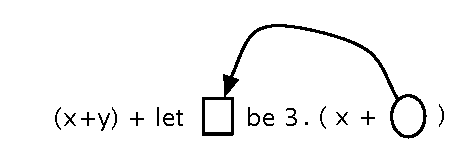
\includegraphics[width=0.8\textwidth]{bd1.pdf}

How do we draw this?  Every binding has a \emph{scope} which is the term that it is applied to.  Any occurrence of $\ttx$ that is outside the scope of an $\ttx$-binder is a free occurrence.  If it is inside the scope of an $\ttx$-binding, it is bound to that $\ttx$-binding.  Sometimes, an $\ttx$-binder sits inside the scope of another $\ttx$-binder:
\begin{displaymath}
  \ttletmac{ 3 }{ \ttx } \ttletmac{ 4 }{ \ttx } (\ttx + 2)
\end{displaymath}
This is called \emph{shadowing}, and the scope of the inner binder is subtracted  from the scope from the outer binder.  So the occurrence of $\ttx$ at the end is bound to the second binder.

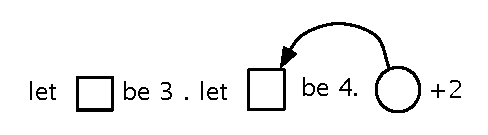
\includegraphics[width=0.8\textwidth]{bd2.pdf}

General rule:
\begin{quotation}
Given an occurrence of $\ttx$, move up the branch of the tree, and as soon as you hit an $\ttx$-binder, that's the place the occurrence is bound to.  If you never hit an $\ttx$-binder, the occurrence is free.
\end{quotation}

\begin{exercise}
  Draw a binding diagram for
  \begin{displaymath}
    \ttletmac{ 3 }{ \ttx } 
 \ttletmac{ (\ttletmac { \ttx+2 }{ \tty } \tty+7) }{ \tty } 
 \ttx + \tty
  \end{displaymath}
\end{exercise}
We write $\bd{M}$ for the binding diagram of $M$.  Two terms with the same binding diagram are \emph{$\alpha$-equivalent}.
\begin{displaymath}
  M \equiv_{\alpha} N \iff \bd{M} = \bd{N}
\end{displaymath}
For example, here is a term $\alpha$-equivalent to the above one:
\begin{displaymath}
  \ttx: \ttint, \tty: \ttint \vdash  (\ttx + \tty) + \ttletmac{ 3 }{ \ttz } (\ttx + \ttz) : \ttint
\end{displaymath}
The only difference is that we've changed a bound identifier.  

Every binding diagram is $\bd{M}$ for some term $M$, because the set of identifiers is infinite.

{\bf Warning} We've learnt two distinct concepts: term and binding diagram.  Unfortunately, people use ``term'' for either of these, and so shall we.   When we want to avoid ambiguity we say \emph{$\alpha$-explicit term} for the former.

{\bf Warning} The way we have defined binding diagram, using squares, circles and arrows, doesn't enable us to meaningfully make definitions by structural recursion over binding diagrams.  As you have learnt in category theory, structural recursion depends on the notion of \emph{initial algebra}.  There are several ways of exhibiting the collection of binding diagrams as an initial algebra, but they are beyond the scope of the course.  For example: Fiore, Plotkin and Turi's paper ``Abstract syntax and variable binding'' (LICS 1999). 





\section{Substitution}
\subsection{Substitution and Binding Diagrams}

An important operation on terms is \emph{substitution}.  If $M$ and $N$ are terms, we write $M[N/\ttx]$ for the term in which we substitute $N$ for $\ttx$ in $M$. For example, if $M$ is $(\ttx+\tty) \times
  3$ and $N$ is $(\tty \times 2)$ then $M[N/\ttx]$ is $((\tty \times
  2)+\tty) \times 3$.  

The preceding paragraph is a slight lie: substitution is actually an operation on \emph{binding diagrams}, not on $\alpha$-explicit terms.  We must remember this in order to perform substitution correctly.
  \begin{enumerate}
  \item Suppose $M$ is $\ttx + \ttletmac{ 3 }{ \ttx } \ttx \times 7$, and $N $ is $\tty \times 2$,  Writing the binding diagrams ensures that we replace only the \emph{free} occurrences.   We therefore obtain
  \begin{displaymath}
M[N/\ttx] = (\tty \times 2) + \ttletmac{ 3 }{ \ttx } \ttx \times 7
\end{displaymath}
  \item Suppose  $M$ is $\ttletmac{ 3 }{ \tty } \ttx + \tty$, and $N$ is $\tty \times 2$.  Writing these as binding diagrams ensures that the free occurrence of $\tty$ in $N$ remains free.  So we obtain
    \begin{displaymath}
M[N/\ttx] = \ttletmac{ 3 }{ \ttz } (\tty \times 2) + \ttz
\end{displaymath}
If we try to substitute naively, we get $\ttletmac{ 3 }{ \tty } (\tty \times 2) + \tty$.  That's the wrong answer, because the free occurrence of $\tty$ in $N$ has been \emph{captured}.  Substitution of binding diagrams is \emph{capture-free}.
  \end{enumerate}
It is desirable to define $M[N/\ttx]$ by structural recursion over the binding diagram $M$, but we are not in a position to do this. 

  \begin{exercise}
    Substitute
    \begin{displaymath}
      \ttletmac{ \ttx+1 }{ \ttx } \ttx + \tty
    \end{displaymath}
 for $\ttx$ in
 \begin{displaymath}
   \ttx + (\ttletmac{ \ttx + 2 }{ \tty } \ttletmac{ \ttx + \tty }{ \ttx } \ttin \ttx+\tty)
 \end{displaymath}
  \end{exercise}


\subsection{The  category of substitutions}

Suppose we have a term $\Gamma \vdash M  : B$, and we want to turn it into a term in context $\Gamma'$, by replacing the identifiers.  For example, we're given the term
\begin{displaymath}
  \ttx:\ttint, \tty:\ttbool, \ttz:\ttint \vdash \ttz + \ttcase \tty \ttof \{\tttrue.\ \ttx+\ttz, \ttfalse.\ \ttx+1 \} : \ttint
\end{displaymath}
and we want to change it to something in the context $\ttu:\ttbool,  \ttx:\ttint, \tty:\ttbool $.

A \emph{substitution} from $\Gamma$ to $\Gamma'$ is a function $k$ taking each identifier $\ttx:A$ in $\Gamma$ to a term (more precisely: a binding diagram) $\Gamma' \vdash k(\ttx):A$.


For example, using the above $\Gamma$ and $\Gamma'$, a substitution from $\Gamma$ to $\Gamma'$ is
\begin{eqnarray*}
  \ttx & \mapsto & 3+\ttx \\
  \tty & \mapsto & \ttu \\
  \ttz & \mapsto & \ttcase \tty \ttof \{ \tttrue.\ \ttx+2, \ttfalse.\ \ttx\}
\end{eqnarray*}
We write $k^{*}M$ for the result of replacing all the free identifiers in $M$ according to $k$ (avoiding capture, of course).  In the above example, we obtain
\begin{displaymath}
  \begin{array}{l}
 \ttu:\ttbool,  \ttx:\ttint, \tty:\ttbool \vdash\\
\beunixt \ttcase \tty \ttof \{ \tttrue.\ \ttx+2, \ttfalse.\ \ttx\}\  + \\ 
\beunixt \ttcase \ttu \ttof \{ \\
 \beunixt \beunixt \tttrue.\ (3+\ttx)+\ttcase \tty \ttof \{ \tttrue.\ \ttx+2, \ttfalse.\ \ttx\}, \\ 
\beunixt \beunixt \ttfalse.\ (3+\ttx)+1 \\
 \beunixt  \} : \ttint
\end{array}
\end{displaymath}


\begin{exercise}
  Apply to the term
  \begin{displaymath}
    \ttx : \ttint \rightarrow \ttint, \tty: \ttint \vdash \ttletmac{ 5 }{ \ttw  } (\ttx \tty) + (\ttx \ttw) : \ttint
  \end{displaymath}
the substitution
\begin{eqnarray*}
  \ttx \mapsto \tty \\
 \tty \mapsto \ttw+1
\end{eqnarray*}
to obtain a term in context
\begin{displaymath}
  \ttw : \ttint, \tty: \ttint \rightarrow \ttint, \ttz:\ttint
\end{displaymath}
\end{exercise}


To form a category, we define
\begin{itemize}
\item the identity subsitution on $\Gamma$ to send each $(\ttx:A) \in \Gamma$ to $\ttx$
\item the composite of substitutions
  \begin{math}
    \xymatrix{
 \Gamma \ar[r]^-{k} & \Gamma' \ar[r]^-{l} & \Gamma''
}
  \end{math}
to send $(\ttx:A) \in \Gamma$ to $l^{*}(k(\ttx))$.
\end{itemize}
We obtain the equations
\begin{eqnarray}
  (k;l)^{*}M & = & l^{*}k^{*}M  \label{eqn:compsubst} \\
  \id_{\Gamma}^{*}M & = & M \label{eqn:idsubst}
\end{eqnarray}
These are pictorially obvious.  We are not in a position to prove them by structural induction over the binding diagram $M$.

The associativity law for composition follows from (\ref{eqn:compsubst}), the left identity law from (\ref{eqn:idsubst}), and the right identity law from 
the equation
\begin{displaymath}
  k^{*} \ttx = k(\ttx)
\end{displaymath}
Therefore contexts and substitutions form a category.




\section{Exercises}

\begin{enumerate}
\item Turn some of the descriptions of integers from the notes into expressions.  Write out binding diagrams and proof trees for these examples (hint: use a large piece of paper in landscape orientation). 
\item What integer is
  \begin{displaymath}
    \begin{array}{l}
    \itletmac{ 3 }{ x } \\ \itletmac{ \ittagl{\lambda y_{\integ}.\, (x + y)} }{ u } \\
 \itletmac{ 4 }{ x }  \\
x + (\itcase u \itof \{ \ittagl{f}\itin f\,2, \ittagr{f}\itin 0 \})
\end{array}
  \end{displaymath}
?
% should simplify to
%   \begin{displaymath}
%     \begin{array}{l}
%     \itlet 3 \itlbe x \itin \\ \itlet \lambda y_{\integ}. (x + y) \itlbe u \itin \\
%  \itlet 4 \itlbe x \itin  \\
%  f2
% \end{array}
%   \end{displaymath}
\item What integer is 
  \begin{displaymath}
    \begin{array}{l}
 \itletmac{ \lambda x_{\integ}.\ \ittagl{\lambda y_{\integ}.\,(x+y)} }{ f } \\
    \itletmac{ f\,0 }{ u }   \\
    \itcase u \itof \{ \\ 
 \betwixt \ittagl{g}\itin \itletmac{ f\,1 }{ v }
   \itcase v \itof \{\ittagl{h}\itin g\,3, \ittagr{h}\itin 0 \},  \\
\betwixt \ittagr{g}\itin 0 \\ \}
 \end{array}
  \end{displaymath}
?
% should simplify to
%   \begin{displaymath}
%     \begin{array}{l}
%  \itlet \lambda x_{\integ}.\ \ittagl{\lambda y_{\integ}.(x+y)} \itlbe f \itin \\
%     \itcase f0 \itof \{ \\ 
%  \betwixt \ittagl{g}.\ 
%    \itcase f1 \itof \{\ittagl{h}.\ g3, \ittagr{h}.\ 0 \},  \\
% \betwixt \ittagr{g}.\ 0 \\ \}
%  \end{array}
%   \end{displaymath}
\item (variant tuple type) For sets $R,R',S,S',S''$, we define $\leftconn(0.R,R';1.S,S',S'')$ to be the set of tuples
  \begin{displaymath}
    \{ \tuple{\lefttagp,x,y} | x \in R, y \in R' \} \cup \{ \tuple{\righttagp,x,y,z} | x \in S, y \in S', z \in S'' \}
  \end{displaymath}
Here 0 and 1 are serving as ``tags''.


Now suppose that for types $A,A',B,B',B''$ we want a type $\leftconn(0.A,A';1.B,B',B'')$ as an operation on types.  Give typing rules for
\begin{itemize}
\item $\tuple{\lefttagp,M,N}$
\item $\tuple{\righttagp,M,N,P}$
\item $\ttcase M \ttof \{\tuple{\lefttagp,\ttx,\tty}.\ N,\ \tuple{\righttagp,\ttx,\tty,\ttz}.\ N'\}$
\end{itemize}
i.e.\ two introduction rules and one elimination rule for $\leftconn(0.A,A';1.B,B',B'')$.
\item (variant function type) For sets $R,R',S,T,T',T'',U$, we define $\rightconn(0.R,R' \vdash S; 1.T,T',T'' \vdash U)$ to be the set of functions that take
  \begin{itemize}
  \item a sequence of arguments $(\lefttagp, x , y)$, where $x \in R$ and $y \in R'$, to an element of $S$
  \item a sequence of arguments $(\righttagp, x, y, z)$, where $x \in T$ and $y \in T'$ and $z \in T''$, to an element of $U$.
  \end{itemize}
% Thus the first argument is always a tag, indicating how many other arguments there are, what their type is, and what the type of the result should be.

Now suppose that for types $A,A',B,C,C',C'',D$ we want a type $\rightconn(0. A, A' \vdash B ; 1. C,C',C'' \vdash D)$ as an operation on types.  Give typing rules for
\begin{itemize}
\item $M\,(\lefttagp,N,N')$
\item $M\,(\righttagp,N,N',N'')$
\item $\lambda \{ (\lefttagp,\ttx_{A},\tty_{B}).\,M, (\righttagp,\ttx_{D},\tty_{E},\ttz_{F}).\,M' \}$
\end{itemize}
i.e.\ two elimination rules and one introduction rule for $\rightconn(0.A, A' \vdash B ; 1. C,C',C'' \vdash D)$
\end{enumerate}



% \section{Substitution again}
% \subsection{Substitutions and Renamings}


% Suppose we have a term $\Gamma \vdash M  : B$, and we want to turn it into a term in context $\Gamma'$, by replacing the identifiers.  For example, we're given the term
% \begin{displaymath}
%   \ttx:\ttint, \tty:\ttbool, \ttz:\ttint \vdash \ttz + \ttcase \tty \ttof \{\tttrue.\ \ttx+\ttz, \ttfalse.\ \ttx+1 \} : \ttint
% \end{displaymath}
% and we want to change it to something in the context $\ttu:\ttbool,  \ttx:\ttint, \tty:\ttbool $.

% \subsection{Replacing Identifiers With Identifiers}

% One way is to  replace identifiers in $\Gamma$ with \emph{identifiers} in $\Gamma'$.  A \emph{renaming} from $\Gamma$ to $\Gamma'$ (beware the direction here) is a function $\theta$ taking each identifier $\ttx:A$ in $\Gamma$ to an identifier $\theta(\ttx):A$ in $\Gamma'$. 

% For example, using the above $\Gamma$ and $\Gamma'$, one renaming from $\Gamma$ to $\Gamma'$ is
% \begin{eqnarray*}
%   \ttx & \mapsto & \ttx \\
%   \tty & \mapsto & \ttu \\
%   \ttz & \mapsto & \ttx
% \end{eqnarray*}
% We write $\theta^{*}M$ for the result of changing all the free identifiers in $M$ according to $\theta$.  In the above example, we obtain
% \begin{displaymath}
%   \ttu:\ttbool,  \ttx:\ttint, \tty:\ttbool \vdash \ttx + \ttcase \ttu \ttof \{\tttrue.\ \ttx+\ttx, \ttfalse.\ \ttx+1 \} : \ttint
% \end{displaymath}

% % \begin{remark}
% %   We can form a category in which an object is a context, and a morphism is a
% %   renaming.  And $(\theta;\phi)^{*}M$ is the same as $\theta^{*} \phi^{*}M$, and $\id^{*}M$ is just $M$.
% % \end{remark}

% % If $\amorphism{\theta}{\Gamma}{\Gamma'}$ is a renaming, and $\ttx$ doesn't appear in $\Gamma$ or $\Gamma'$, we can define $\amorphism{\theta,\ttx:A}{\Gamma,\ttx:A}{\Gamma',\ttx:A}$.  It maps $\ttx$ to $\ttx$, and otherwise is exactly the same as $\theta$.

% % We can define $\theta^{*}M$ by induction on $M$, and that's very useful for proving theorems about it.  Some clauses are easy:

% \begin{exercise}
%   Apply to the term
%   \begin{displaymath}
%     \ttx : \ttint \rightarrow \ttint, \tty: \ttint \vdash \ttlet 5 \ttlbe \ttw \ttin (\ttx \tty) + (\ttx \ttw) : \ttint
%   \end{displaymath}
% the renaming
% \begin{eqnarray*}
%   \ttx \mapsto \tty \\
%  \tty \mapsto \ttw
% \end{eqnarray*}
% to obtain a term in context
% \begin{displaymath}
%   \ttw : \ttint, \tty: \ttint \rightarrow \ttint, \ttz:\ttint
% \end{displaymath}
% \end{exercise}

% \subsection{Replacing Identifiers With Terms}

% The second example is called \emph{substitution}, where we replace each identifier in $\Gamma$ with a \emph{term} in context $\Gamma'$. 
%  A \emph{substitution} from $\Gamma$ to $\Gamma'$ is a function $k$ taking each identifier $\ttx:A$ in $\Gamma$ to a term $\Gamma' \vdash k(\ttx):A$.


% For example, using the above $\Gamma$ and $\Gamma'$, a substitution from $\Gamma$ to $\Gamma'$ is
% \begin{eqnarray*}
%   \ttx & \mapsto & 3+\ttx \\
%   \tty & \mapsto & \ttu \\
%   \ttz & \mapsto & \ttcase \tty \ttof \{ \tttrue.\ \ttx+2, \ttfalse.\ \ttx\}
% \end{eqnarray*}
% We write $k^{*}M$ for the result of replacing all the free identifiers in $M$ according to $k$ (avoiding capture, of course).  In the above example, we obtain
% \begin{displaymath}
%   \begin{array}{l}
%  \ttu:\ttbool,  \ttx:\ttint, \tty:\ttbool \vdash\\ \ttcase \tty \ttof \{ \tttrue.\ \ttx+2, \ttfalse.\ \ttx\}  + \\ \ttcase \ttu \ttof \{\tttrue.\ (3+\ttx)+\ttcase \tty \ttof \{ \tttrue.\ \ttx+2, \ttfalse.\ \ttx\}, \\ \ttfalse.\ (3+\ttx)+1 \} : \ttint
% \end{array}
% \end{displaymath}

% % \begin{remark}
% %   We can form a category of contexts and substitutions, where composition is defined by substitution.  And $(k;l)^{*}M$ is the same as $k^{*}l^{*}M$, and $\id^{*}M$ is the same as $M$.  Furthermore, this contains the category of renamings as a subcategory
% % \end{remark}

% \begin{exercise}
%   Apply to the term
%   \begin{displaymath}
%     \ttx : \ttint \rightarrow \ttint, \tty: \ttint \vdash \ttlet 5 \ttlbe \ttw \ttin (\ttx \tty) + (\ttx \ttw) : \ttint
%   \end{displaymath}
% the substitution
% \begin{eqnarray*}
%   \ttx \mapsto \tty \\
%  \tty \mapsto \ttw+1
% \end{eqnarray*}
% to obtain a term in context
% \begin{displaymath}
%   \ttw : \ttint, \tty: \ttint \rightarrow \ttint, \ttz:\ttint
% \end{displaymath}
% \end{exercise}

% An important special kind of substitution is one that maps each identifier to an identifier; this is called a \emph{renaming}.  An even more special case is the inclusion from $\Gamma$ to $\Gamma'$, where $\Gamma \subseteq \Gamma'$.  This is called \emph{weakening}.  You will often see it expressed as a proposition.
% \begin{proposition} \label{prop:weaken}
%   If $\Gamma \subseteq \Gamma'$ and $\Gamma \vdash M : A$ then $\Gamma' \vdash M:A$.
% \end{proposition}
% This is proved by induction, using the fact that if $\Gamma \subseteq \Gamma'$ then $\Gamma,\ttx:B \subseteq \Gamma', \ttx:B$.

% \subsection{Substitution by Induction}

% Let us think how to define substitution on terms (rather than on binding diagrams) by induction.   Some of the inductive clauses are easy:
% \begin{eqnarray*}
%   k^{*}3 & = & 3 \\
%   k^{*}(M+N) & = & k^{*}M + k^{*}N \\
%   k^{*} \ttx & = & k(\ttx)
% \end{eqnarray*}
% But what about substituting into a $\ttlet$ expression?  Let's first remember the typing rule for $\ttlet$:
% \begin{displaymath}
% \begin{prooftree}
%   \Gamma \vdash M:A \betwixt \Gamma, \ttx:A \vdash N:B \justifies \Gamma \vdash
%   \ttlet M \ttlbe \ttx \ttin N : B
% \end{prooftree}
% \end{displaymath}

% We define
% \begin{displaymath}
%   k^{*} (\ttlet M \ttlbe \ttx \ttin N) = \ttlet k^{*}M \ttlbe \ttw \ttin (k,\ttx \mapsto \ttw)^{*}N
% \end{displaymath}
%  where $\ttw$ is some identifier that doesn't appear in $\Gamma'$, and the substitution $\amorphism{k,\ttx\mapsto \ttw}{\Gamma,\ttx:A}{\Gamma',\ttx:A}$ is defined to map $(\tty:B) \in \Gamma$ (provided $\tty \not= \ttx$) to
%    $k(\tty)$, and $\ttx$ to $\ttw$. Note the use of Proposition~\ref{prop:weaken} in this definition: $\Gamma',\ttw:A \vdash k(\tty):B$ follows from $\Gamma' \vdash k(\tty):B$ since $\ttw \not\in \Gamma'$.


% A consequence of this is that if you want to prove a theorem about substitution, you'll first have to prove it for renaming, or at least for weakening.


% % How do we define renaming inductively?  Again, some of the inductive clauses are easy:
% % \begin{eqnarray*}
% %   \theta^{*}3 & = & 3 \\
% %   \theta^{*}(M+N) & = & \theta^{*}M + \theta^{*}N \\
% %   \theta^{*} \ttx & = & \theta(\ttx)
% % \end{eqnarray*}
% % For $\ttlet$, we want to define
% % \begin{displaymath}
% %   \theta^{*} (\ttlet M \ttlbe \ttx \ttin N) = \ttlet \theta^{*}M \ttlbe \ttx \ttin (\theta,\ttx:A)^{*}N
% % \end{displaymath}
% % where the renaming morphism $\amorphism{\theta,\ttx:A}{\Gamma,\ttx:A}{\Gamma',\ttx:A}$ maps $\ttx$ to $\ttx$, and otherwise is the same as $\theta$.  



% % In summary, the definition of substitution goes in 4 stages:
% % \begin{itemize}
% % \item define $\theta,\ttx:A$
% % \item define renaming by induction
% % \item define $k,\ttx:A$
% % \item define substitution by induction.
% % \end{itemize}

% Next we define
% \begin{itemize}
% \item the identity subsitution on $\Gamma$ to send each $(\ttx:A) \in \Gamma$ to $\ttx$
% \item the composite of substitutions
%   \begin{math}
%     \xymatrix{
%  \Gamma \ar[r]^{k} & \Gamma' \ar[r]^{l} & \Gamma''
% }
%   \end{math}
% to send $(\ttx:A) \in \Gamma$ to $l^{*}(k(\ttx))$.
% \end{itemize}

% While we have defined subsitution for terms, this involves an arbitrary choice of fresh identifier.  Because of this, it is only on binding diagrams that we obtain a \emph{canonical} operation.  Furthermore, provided we work with binding diagrams (or up to $\alpha$-equivalence), we have equations:
% \begin{eqnarray*}
%   (k;l)^{*}M & = & l^{*}k^{*}M \\
%   \id_{\Gamma}^{*}M & = & M
% \end{eqnarray*}
% It follows that contexts and substitutions form a category, i.e.\ composition satisfies the associativity, left unital and right unital laws.  

% \begin{proposition}
%   \begin{enumerate}
% \item $(k;l)^{*}M$ is the same as $l^{*}k^{*}M$, and $\id_{\Gamma}^{*}M$ is the same as $M$. 
% %   \item Contexts and renamings form a category.
% %  \item $(\theta;\phi)^{*}M$ is the same as $\theta^{*} \phi^{*}M$, and $\id^{*}M$ is just $M$.
%   \item Contexts and substitutions form a category---i.e.\ composition satisfies the associativity, left unital and right unital laws.
% %  \item There is an obvious functor $\iota$ from the category of contexts and renamings to the category of contexts and substitutions. \item For any renaming $\theta$, we have $(\iota \theta)^{*} M = \theta^{*}M$.
% \end{enumerate}
% \end{proposition}


\section{Evaluation Through $\beta$-reduction}

% $\lambda$-calculus is not just a set of terms, it provides \emph{equations} between terms.  We write 
% \begin{displaymath}
%   \Gamma \vdash M = N : B
% \end{displaymath}
% Intuitively, this is supposed to mean that, whatever the identifiers in $\Gamma$ are defined to be, $M$ and $N$ have the same \emph{meaning} (even though they're different expressions).

Intuitively, a $\beta$-reduction means simplification.  I'll write $M \rightsquigarrow N$ to mean that $M$ can be simplified to $N$.  We begin with some arithmetic simplifications, sometimes called \emph{$\delta$-reductions}:
\begin{eqnarray*}
  \underline{m} + \underline{n} & \rightsquigarrow & \underline{m+n} \\
  \underline{m} \times  \underline{n} & \rightsquigarrow & \underline{m\times n} \\
  \underline{m} > \underline{n} & \rightsquigarrow & \tttrue \mbox{ if $m>n$} \\
 \underline{m} > \underline{n} & \rightsquigarrow & \ttfalse \mbox{ if $m\leqslant n$} \\
\end{eqnarray*}
There is a $\beta$-reduction rule for local definitions:
\begin{eqnarray*}
  \ttletmac{ M }{ \ttx } N  & \rightsquigarrow & N[M/\ttx]
\end{eqnarray*} 


But the most interesting are the $\beta$-reductions for all the types.  The rough idea is: if you use an introduction rule and then, immediately, use an elimination rule, then they can be simplified.

For the boolean type, the $\beta$-reduction rule is
\begin{eqnarray*}
  \ttcase \tttrue \ttof \{ \tttrue. N, \ttfalse. N' \} & \rightsquigarrow & N \\
  \ttcase \ttfalse \ttof \{ \tttrue. N, \ttfalse. N' \} & \rightsquigarrow & N' 
\end{eqnarray*}

For the type $A \times B$, if we use projections the $\beta$-reduction rule is
\begin{eqnarray*}
  \projl \pair{M}{M'} & \rightsquigarrow & M \\
 \projr \pair{M}{M'} & \rightsquigarrow & M'
\end{eqnarray*}

If we use pattern-matching, the $\beta$-reduction rule is
\begin{eqnarray*}
  \ttsplit \pair{M}{M'} \ttspof \pair{\ttx}{\tty} \ttin N & \rightsquigarrow & N[M/\ttx,M'/\tty]
\end{eqnarray*}
% and for the type $1$ it is
% \begin{eqnarray*}
%   \ttcase \tuple{\,} \ttof \tuple{\,} \ttin N & \rightsquigarrow & N
% \end{eqnarray*}

For the type $A + B$, the $\beta$-reduction rule is
\begin{eqnarray*}
  \ttcase \tttagl{M} \ttof \{ \tttagl{\ttx} \ttin N, \tttagr{\tty} \ttin N' \} & \rightsquigarrow & N[M/\ttx] \\
  \ttcase \tttagr{M} \ttof \{ \tttagl{\ttx} \ttin N, \tttagr{\tty} \ttin N' \} & \rightsquigarrow & N'[M/\tty] \\
\end{eqnarray*}

For the type $A \rightarrow B$, the $\beta$-reduction rule is 
\begin{eqnarray*}
  (\lambda \ttx_{A}.\, M) N & \rightsquigarrow & M[N/\ttx]
\end{eqnarray*}

A term which is the left-hand-side of a $\beta$-reduction is called a \emph{$\beta$-redex}.

To simplify a term $M$ we pick a subterm that's a $\beta$-redex or $\delta$-redex, and reduce it.  If $M$ has no subterm that's a $\beta$- or $\delta$-redex, it's said to be $\beta\delta$-normal.

\begin{proposition}
  A \emph{closed} term $M$ that is $\beta\delta$-normal must have an introduction rule at the root. In other words, it must have one of the following forms:
  \begin{displaymath}
    \tttrue \bnf \ttfalse \bnf \underline{n} \bnf \tuple{\,} \bnf \tuple{M,N} \bnf \ttinl M \bnf \ttinr M \bnf \lambda \ttx_{A}.\, M 
  \end{displaymath} 
\end{proposition}
We should prove the first part by induction on $M$ (but it's a binding diagram so we're not in a position to do so).

\begin{proposition}(Strong normalization of $\beta,\delta$-reduction)  \hfill
There is no infinite sequence of $\beta$- and $\delta$-reductions:
  \begin{displaymath}
    M_0 \rightsquigarrow M_1 \rightsquigarrow M_2 \rightsquigarrow \cdots
  \end{displaymath}  
\end{proposition}

\begin{proposition}(Confluence of $\beta,\delta$-reduction)\label{prop:confluence}  \hfill
For a term $M$, if $M \rightsquigstar N$ and $M \rightsquigstar N'$, then there is a term $P$ such that $N \rightsquigstar P$ and $N' \rightsquigstar P$.
\end{proposition}
Confluence is also called the \emph{Church-Rosser} property.  It does not make use of types and holds even for untyped systems.

Thus given a term $M$, we simplify it by picking a $\beta$- or $\delta$-redex subterm, if there is one, and reducing it.  We do this again and again, and by strong normalization we eventually reach $\beta\delta$-normal form.  By confluence this $\beta\delta$-normal form does not depend on the choice of redex suterms.  And if $\vdash M : \ttint$, we know that the $\beta\delta$-normal form must be of the form $\underline{n}$.

\begin{exercise}
  All the sums that we did can be turned into expressions and evaluated using $\beta$-reduction.  Try:
  \begin{enumerate}
  \item $\ttletmac{ \pair{5}{\pair{2}{\tttrue}} }{ \ttx } \projl \ttx + \projl (\ttsplit \ttx \ttspof \pair{\tty}{\ttz} \ttin \ttz)$
  \item $
    \begin{array}{l}
\ttcase (\ttcase (3<7) \ttof \{\tttrue.\ \tttagr{8+1}, \ttfalse.\ \tttagl{2} \}) \ttof \\
\{ \tttagl{\ttu}.\ \ttu+8, \tttagr{\ttu}.\ \ttu+3 \} \\
\end{array}
$
  \item $((\lambda \ttf_{\ttint \rightarrow \ttint}. \lambda \ttx_{\ttint}. (\ttf(\ttf\ttx)))\lambda \ttx_{\ttint}. (\ttx+3))2$
  \end{enumerate}
\end{exercise}

\section{$\eta$-expansion}

The $\eta$-expansion laws express the idea that
\begin{itemize}
\item everything of type $\ttbool$ is $\tttrue$ or $\ttfalse$
\item everything of type $A \times B$ is a pair $\pair{x}{y}$
\item everything of type $A + B$ is a pair $\tttagl{x}$ or a pair $\tttagr{x}$
\item everything of type $A \rightarrow B$ is a function.
\end{itemize}
They are given by first applying an elimination, then an introduction (the opposite of $\beta$-reduction).

Let's begin with the type $\ttbool$.  Suppose we have a term $\Gamma \vdash M: \ttbool$.  Then for any term $\Gamma, \ttz:\ttbool \vdash N:B$, we can expand $N[M/\ttz]$ to 
\begin{displaymath}
  \ttcase M \ttof \{ \tttrue.\ N[\tttrue/\ttz],\ttfalse.\ N[\ttfalse/\ttz] \}\end{displaymath}
The reason this ought to be true is that, whatever we define the identifiers in $\Gamma$ to be, $M$ will be either $\tttrue$ or $\ttfalse$.  Either way, both sides should be the same.


%  Suppose we have a term $\Gamma \vdash M : \ttbool$, and another term $\Gamma, \ttz: \ttbool \vdash N : B$.  Then $N[M/\ttz]$ can be expanded into
% \begin{displaymath}
%   \ttcase M \ttof \{ \tttrue.\ N[\tttrue/\ttz,\ttfalse/\ttz]
% \end{displaymath}
% The reason this ought to be true is that, whatever we define the identifiers in $\Gamma$ to be, $N$ will be either $\tttrue$ or $\ttfalse$.  Either way, both sides should be the same.

What about $A \times B$?  If we're using projections, then any $\Gamma \vdash M : A \times B$ can be $\eta$-expanded to $\pair{\projl M}{\projr M}$.  

And if we're using pattern-match, for terms $\Gamma \vdash M:A \times B$ and $\Gamma, \ttz:A \times B \vdash N : C$, we can expand $N[M/\ttz]$ into 
\begin{displaymath}
  \ttsplit M \ttspof \pair{\ttx}{\tty}.\ N[\pair{\ttx}{\tty}/\ttz]
\end{displaymath}
where $\ttx,\tty \not\in \Gamma$ and $\ttx \not= \tty$.

For $A + B$, it's similar.  Suppose $\Gamma \vdash M:A+B$ and $\Gamma, \ttz:A+B  \vdash N : C$.  Then $N[M/\ttz]$ can be expanded into
\begin{displaymath}
  \ttcase M \ttof \{ \tttagl{\ttx}.\ N[\tttagl{\ttx}/\ttz], \tttagr{\tty}.\ N[\tttagr{\tty}/\ttz] \}
\end{displaymath}
where $\ttx,\tty \not\in\Gamma$.

And finally, $A \rightarrow B$.  Any term $\Gamma \vdash M : A \rightarrow B$ can be expanded as
\begin{displaymath}
\lambda \ttx_{A}.\, (M \ttx)
\end{displaymath}
where $\ttx \not\in \Gamma$.

\begin{exercise}
  Take the term
  \begin{displaymath}
    \ttf: (\ttint + \ttbool) \rightarrow (\ttint + \ttbool) \vdash     \ttf: (\ttint + \ttbool) \rightarrow (\ttint + \ttbool)
  \end{displaymath}
Apply an $\eta$-expansion for $\rightarrow$, then for $+$, then for $\ttbool$.
\end{exercise}





\section{Equality}

$\lambda$-calculus isn't just a set of terms; it comes with an equational theory.  If $\Gamma \vdash M : B$ and $\Gamma \vdash N  : B$, we write $\Gamma \vdash M \eqbe N  :B$ to express the intuitive idea that, no matter what we define the identifiers in $\Gamma$ to be, $M$ and $N$ have the same ``meaning'' (even though they're different expressions).  

First of all we need rules to say that this is an equivalence relation:
\begin{displaymath}
  \begin{array}{ccc}
    \begin{prooftree}
      \Gamma \vdash M : B
      \justifies
      \Gamma \vdash M \eqbe M : B
    \end{prooftree} & & 
    \begin{prooftree}
      \Gamma \vdash M \eqbe N : B
      \justifies
      \Gamma \vdash N \eqbe M : B
    \end{prooftree} \\ \\
    \begin{prooftree}
      \Gamma \vdash M \eqbe N : B \betwixt \Gamma \vdash N \eqbe P : B
      \justifies
      \Gamma \vdash M \eqbe P : B
    \end{prooftree}
  \end{array}
\end{displaymath}
Secondly, we need rules to say that this is \emph{compatible}---preserved by every construct:
\begin{displaymath}
  \begin{prooftree}
    \Gamma \vdash M \eqbe M' : A \betwixt \Gamma, \ttx:A \vdash N \eqbe N' : B
    \justifies
    \Gamma \vdash \ttletmac{ M }{ \ttx } N \eqbe \ttletmac{ M' }{ \ttx } N' : B
  \end{prooftree}
\end{displaymath}
and so forth.  A compatible equivalence relation is often called a \emph{congruence}.

Thirdly, each of the $\beta$-reductions that we've seen is an axiom of this theory.
\begin{displaymath}
  \begin{array}{c}
    \begin{prooftree}
      \Gamma \vdash N : B \betwixt \Gamma \vdash N' : B \justifies \Gamma \vdash
      \ttcase \tttrue \ttof \{ \tttrue.\ N, \ttfalse.\ N' \} \eqbe N  : B
\end{prooftree}
   \\ \\
  \begin{prooftree}
    \Gamma, \ttx:A \vdash M : B \betwixt \Gamma \vdash N : A
    \justifies
    \Gamma \vdash (\lambda \ttx_{A}. M) N \eqbe M[N/\ttx] : B
  \end{prooftree}
\end{array}
\end{displaymath}

Fourthly, each of the $\eta$-expansions is an axiom of the theory, e.g.
\begin{displaymath}
  \begin{prooftree}
    \Gamma \vdash M : A \rightarrow B
    \justifies
    \Gamma \vdash M \eqbe \lambda \ttx_{A}.\, (M \ttx) : A \rightarrow B
  \end{prooftree}
\end{displaymath}
where $\ttx \not\in \Gamma$.

% But in the case of the $\eta$-expansions involving pattern-matching, we need to generalize them slightly.  The reason is that we want to prove
\begin{proposition}\label{prop:substeq}
  If $\Gamma \vdash M \eqbe N : B$ and $\amorphism{k}{\Gamma}{\Gamma'}$ is a substitution, then $\Gamma' \vdash k^{*}M \eqbe k^{*}N : B$
\end{proposition}
% Consequently, the $\eta$-law for $\ttbool$ looks like this:
% \begin{displaymath}
%   \begin{prooftree}
%     \Gamma \vdash M : \ttbool \betwixt \Gamma, \ttz:\ttbool \vdash N : C
%     \justifies
%     \begin{array}{l}
%     \Gamma \vdash N[M/\ttz] \eqbe \\
%  \betwixt \ttcase M \ttof \{ \tttrue. N[\tttrue/\ttz], \ttfalse. N[\ttfalse/\ttz] \} \\
%  \betwixt  : C
%   \end{array}
%   \end{prooftree}
% \end{displaymath}
% and similarly for the other pattern-matching laws.  We can then prove Prop.~\ref{prop:substeq}.

\section{Exercises}

\begin{enumerate}
\item Suppose that $\Gamma \vdash M : \ttbool$ and $\Gamma \vdash N_{0}, N_{1},
  N_{2}, N_{3} : C$.  Show that
\begin{displaymath}
  \begin{array}{l}
  \Gamma \vdash \ttcase M \ttof  \{  \\\betwixt \tttrue.\ \ttcase M \ttof \{\tttrue. N_{0}, \ttfalse.N_{1} \}, \\ \betwixt\ttfalse.\ \ttcase M \ttof \{\tttrue. N_{2}, \ttfalse.N_{3} \} \\ \}  \\
 \eqbe \ttcase M \ttof \{ \tttrue. N_{0}, \ttfalse. N_{3} \} : C
\end{array}
\end{displaymath}
\item Show that $\tttagl{-}$ is injective, i.e.\ if $\Gamma \vdash M, M' : A$ and $\Gamma
\vdash \tttagl{M} \eqbe \tttagl{M'} : A + B$ then $\Gamma \vdash M \eqbe M' : A$.
\item Write down the $\eta$-law for the $0$ type.
\item A typing context $\Gamma$ is \emph{inconsistent} if there is a term $\Gamma \vdash M : 0$.  Show that if $\Gamma$ is inconsistent then for every type $A$ there is a unique (up to $\eqbe$) term $\Gamma \vdash N : A$.
\item Given a term $\Gamma, \ttx:A \vdash M : 0$, show that it is an ``isomorphism'' in the sense that there is a term $\Gamma, \tty : 0 \vdash N : A$ satisfying
  \begin{eqnarray*}
    \Gamma, \tty : 0 \vdash M[N / \ttx] & \eqbe & \tty : 0 \\
    \Gamma, \ttx: A \vdash N[M / \tty] & \eqbe & \ttx : A
  \end{eqnarray*}
\item Give $\beta$ and $\eta$ laws for $\leftconn(0.A,A';1.B,B',B'')$ and for $\rightconn(0.A,A' \vdash B; 1.C,C',C'' \vdash D)$.  (See yesterday's exercises for a description of these types.)
\end{enumerate}


\section{Denotational Semantics}
\subsection{Denotation of Terms}

Now we relate our syntax to the ``real'' world of sets and functions.

The first step: to each type $A$, we associate a set $\seman{A}$.  This is by structural recursion on $A$.
\begin{eqnarray*}
  \seman{\ttint} & = & \integ \\
  \seman{\ttbool} & = & \bool \\
  \seman{A+B} & = & \seman{A} + \seman{B} \\
 \seman{0} & = & 0 \\
\seman{A \times B} & = &  \seman{A} \times \seman{B} \\
\seman{1} & = & 1 \\
  \seman{A\rightarrow B} & = & \seman{A} \rightarrow \seman{B} 
\end{eqnarray*}

Recall that a \emph{typing context} $\Gamma$ is a set of distinct identifiers with types e.g.\ $\ttx:A, \tty:B$.

A \emph{syntactic environment} for $\Gamma$ provides, for each identifier $\ttx:A$ in $\Gamma$, a closed term of type $A$.   (If you like, it's a substitution from $\Gamma$ to the empty context.)

A \emph{semantic environment} for $\Gamma$ provides, for each identifier $\ttx:A$ in $\Gamma$, an element of $\seman{A}$.

For example:
\begin{displaymath}
  \ttx: \ttint \rightarrow \ttint, \tty:\ttbool
\end{displaymath}
is a typing context.

\begin{eqnarray*}
  \ttx & \mapsto & \lambda \ttx_{\ttint}. (\ttx + 1) \\
 \tty & \mapsto & \tttrue
\end{eqnarray*}
is a syntactic environment for that context.

\begin{eqnarray*}
  \ttx & \mapsto & \lambda x_{\integ}. (x + 1) \\
 \tty & \mapsto & \ittrue
\end{eqnarray*}
is a semantic environment for that context.


We define $\seman{\Gamma}$ to be the set of semantic environments for $\Gamma$.  (This is \emph{after} defining the semantics of types.)  So we have bijections:
\begin{eqnarray*}
  \seman{\varepsilon} & \cong & 1 \\
  \seman{\Gamma,\ttx:A} & \cong & \seman{\Gamma} \times \seman{A} \betwixt \betwixt \mbox{ (provided $\ttx \not \in \Gamma$)}
\end{eqnarray*}

Now suppose we have a term $\Gamma \vdash M : B$.  The denotation of $M$ provides, for each semantic environment $\rho \in \seman{\Gamma}$, an element $\seman{M}\rho \in \seman{B}$.  So we can say
\begin{displaymath}
  \amorphism{\seman{M}}{\seman{\Gamma}}{\seman{B}}
\end{displaymath}
To be completely precise we should write $\seman{\Gamma \vdash M : B}$ rather than $\seman{M}$ but I will usually not bother to do this.  

This denotation is defined by structural recursion on the proof of $\Gamma \vdash M : B$.  For example,
\begin{displaymath}
\begin{array}{c}
  \seman{\ttcase M \ttof \{\tttagl{\ttx}. N, \tttagr{\tty}. N' \} }\rho \\ = \\  \itcase \seman{M}\rho \itof \{ \ittagl{x}.\seman{N}(\rho, \ttx \mapsto x), \ittagr{y}.\seman{N'}(\rho, \tty \mapsto y) \}
\end{array}
\end{displaymath}


\subsection{Complications}


\begin{itemize}
\item If we are using implicit typing, it is necessary to show that the denotation of $\Gamma \vdash M : B$ is independent of the derivation.  This property is called \emph{coherence}.
\item We have given the denotation of $\alpha$-explicit terms.  It's also possible to give the denotation of binding diagrams, by structural recursion, although we are not in a position to do so.  We then prove for any term $\Gamma \vdash M  :B $ that 
  \begin{displaymath}
    \seman{M} = \seman{\bd{M}}
  \end{displaymath}
\end{itemize}


\subsection{Substitution Lemma}

Next, given a substitution $\amorphism{k}{\Gamma}{\Gamma'}$, we obtain a function $\amorphism{\seman{k}}{\seman{\Gamma'}}{\seman{\Gamma}}$ (note the change of direction).  It maps $\rho \in \seman{\Gamma'}$ to the semantic environment for $\Gamma$ that takes each identifier $\ttx:A$ in $\Gamma$ to $\seman{k(\ttx)}\rho$.

We use this to formulate a \emph{substitution lemma}.  
\begin{lemma}
Let $\Gamma \vdash M : B$ be a term. \newline
 For any semantic environment $\rho$ for $\Gamma'$ we have
  \begin{eqnarray*}
    \seman{k^{*}M}\rho & = & \seman{M}(\seman{k}\rho)
  \end{eqnarray*}
  As a diagram:
  \begin{displaymath}
    \xymatrix{
      \seman{\Gamma'} \ar[d]_{\seman{k}} \ar[dr]^{\seman{k^*M}} & \\
      \seman{\Gamma} \ar[r]_-{\seman{M}} & \seman{B} \\
    }
  \end{displaymath}
\end{lemma}

This should be proved by structural induction over the binding diagram $M$.  Once again, we are not in a position to do this.

As a special case of the substitution lemma, we can express $\seman{M[N/\ttx]}$ in terms of $\seman{M}$ and $\seman{N}$:
\begin{displaymath}
  \seman{M[N/\ttx]}\rho = \seman{M}(\rho,\ttx\mapsto \seman{N}\rho)
\end{displaymath}

Armed with the substitution lemma, it is easy to prove the soundness of all our equations:
\begin{proposition}
  If $\Gamma \vdash M \eqbe N : A$ then $\seman{M} = \seman{N}$. 
\end{proposition}

Now, let's write
\begin{itemize}\item 
  $\termsofbe{\Gamma \vdash B}$ to mean the set of $\eqbe$ equivalence classes of terms $\Gamma \vdash
  M : B$ 
\item $\seman{\Gamma \vdash B}$ to mean the set
  of functions from $\seman{\Gamma}$ to $\seman{B}$.
\end{itemize}
Our denotational semantics provides a function
\begin{displaymath}
  \termsofbe{\Gamma \vdash B} \to \seman{\Gamma \vdash B}
\end{displaymath}

\section{Leftist and rightist connectives}
\subsection{Reversible rules}

Each connective (except $\ttint$) has a \emph{reversible rule}.  For $+$ it is
\begin{displaymath}
  \begin{prooftree}
    \Gamma, A \vdash C \betwixt \Gamma, B \vdash C
    \Justifies
    \Gamma, A+B \vdash C
  \end{prooftree}
\end{displaymath}
At the syntactic level, this means that we have a bijection 
\begin{eqnarray*}
\termsofbe{\Gamma, \ttx:A \vdash C} \beunixt\times\beunixt \termsofbe{\Gamma, \tty :B \vdash C} & \beunixt\cong\beunixt &  \termsofbe{\Gamma, \ttz:A+B \vdash C}
\end{eqnarray*}
assuming $\ttx,\tty,\ttz \not \in \Gamma$.
\begin{itemize}
\item A pair of equivalence classes $[\Gamma, \ttx:A \vdash M :  C]_{\beta\eta}$ and $[\Gamma, \tty: B \vdash M' : C]_{\beta\eta}$ corresponds to 
  \begin{displaymath}
    [\Gamma, \ttz:A + B \vdash \ttcase \ttz \ttof \{ \ttinl \ttx.\, M, \ttinr \tty.\ M'\} \ :\ C]_{\beta\eta}
  \end{displaymath}
\item Conversely, an equivalence class $[\Gamma, \ttz: A + B \vdash N : C]_{\beta\eta}$ corresponds to $[\Gamma, \ttx:A \vdash N[\ttinl \ttx/\ttz]]_{\beta\eta}$ and $[\Gamma, \tty :B \vdash N[\ttinr \tty/\ttz]]_{\beta\eta}$.
\end{itemize}
The fact that these operations are inverse follows from the $\beta$- and $\eta$-laws.

At the semantic level, we have a bijection 
\begin{eqnarray*}
\seman{\Gamma, \ttx:A \vdash C} \beunixt\times\beunixt \seman{\Gamma, \tty:B \vdash C} & \beunixt\cong\beunixt & \seman{\Gamma, \ttz:A + B \vdash C}
\end{eqnarray*}
assuming $\ttx,\tty,\ttz\not\in\Gamma$. More generally, for any \emph{sets} $R, S, T, U$, we have a bijection
\begin{eqnarray*}
  ((R \times S) \to U) \beunixt\times\beunixt ((R \times T) \to U) & \beunixt\cong\beunixt & (R \times (S + T)) \to U
\end{eqnarray*}

The reversible rule for $\ttbool$ is similar:
\begin{displaymath}
  \begin{prooftree}
    \Gamma \vdash C \betwixt \Gamma \vdash C
    \Justifies
    \Gamma, \ttbool \vdash C
  \end{prooftree}
\end{displaymath}



For $\to$ the reversible rule is
\begin{displaymath}
  \begin{prooftree}
    \Gamma, A \vdash B
    \Justifies
    \Gamma \vdash A \rightarrow B
  \end{prooftree}
\end{displaymath}
At the syntactic level, this means that we have a bijection 
\begin{eqnarray*}
\termsofbe{\Gamma, \ttx:A \vdash B} & \beunixt\cong\beunixt & \termsofbe{\Gamma \vdash A \to B}
\end{eqnarray*}
assuming $\ttx \not \in \Gamma$.
\begin{itemize}
\item An equivalence class $[\Gamma, \ttx :A \vdash M : B]_{\beta\eta}$ corresponds to $[\Gamma \vdash \lambda \ttx_{A} .\ M : A \to B]_{\beta\eta}$.
\item Conversely, an equivalence class $[\Gamma \vdash N : A \to B]_{\beta\eta}$ corresponds to $[\Gamma, \ttx : A \vdash N \ttx :  B]_{\beta\eta}$.
\end{itemize}
The fact that these operations are inverse follows from the $\beta$- and $\eta$-laws.

At the semantic level, we have a bijection 
\begin{eqnarray*}
\seman{\Gamma, A \vdash B} & \beunixt\cong\beunixt & \seman{\Gamma \vdash A \to B}
\end{eqnarray*}
assuming $\ttx \not\in \Gamma$.  
More generally, for any \emph{sets} $R, S , T$, we have a bijection
\begin{eqnarray*}
( R \times S ) \to T & \beunixt\cong\beunixt & R \to (S \to T)
\end{eqnarray*}

For $\times$ there are two reversible rules, just as there are two versions of the elimination rules.  The one that fits projections is
\begin{displaymath}
  \begin{prooftree}
    \Gamma \vdash A \betwixt \Gamma \vdash B
    \Justifies
    \Gamma \vdash A \times B
  \end{prooftree}
\end{displaymath}
The one that fits pattern-matching is
\begin{displaymath}
  \begin{prooftree}
    \Gamma, A, B \vdash C
    \Justifies
    \Gamma, A \times B \vdash C
  \end{prooftree}
\end{displaymath}
We describe $\ttbool, +, 0, \times, 1$ as \emph{leftist} connectives because they appear to the left of $\vdash$ in the conclusion of a reversible rule.  We likewise describe $\rightarrow, \times, 1$ as \emph{rightist}.  Note that the connectives $\times, 1$ are bipartisan.  

Is it surprising that product type with projection syntax should resemble a function type?  Think of $\pair{M}{N}$ as a function that maps  $0$ to $M$ and $1$ to $N$.  Then $\projl M$ is $M$ applied to $0$, and $\projr M$ is $M$ applied to $1$.   

\subsection{Naturality}

An important property of the reversible rules is that they are ``natural''.  (This is closely linked to category theory, but we shall not explore this connection here.)

Take, for example, the reversible rule for $\to$.
\begin{displaymath}
  \begin{prooftree}
    \Gamma, A \vdash B
    \Justifies
    \Gamma \vdash A \rightarrow B
  \end{prooftree}
\end{displaymath}
This is \emph{natural in $\Gamma$}, in a sense I shall explain. 

A substitution $k \ :\ \Gamma \to \Gamma'$ gives rise to an operation $k^{*}$, sending a term $\Gamma, \Delta \vdash  M : C$ to a term term $\Gamma', \Delta \vdash M[k(\ttx)/\ttx]_{\ttx \in \Gamma} : C$.  (Assuming $\Delta$ disjoint from $\Gamma$ and from $\Gamma'$.)  

Given a term $\Gamma, \ttx:A \vdash M :B$, we can move down the rule and then apply $k^*$.  Or we can apply $k^*$ and then move down the rule.  Naturality says we get the same result.  This is obvious.

For a leftist example, take the reversible rule for $A + B$.
\begin{displaymath}
  \begin{prooftree}
    \Gamma, A \vdash C \betwixt \Gamma, B \vdash C
    \Justifies
    \Gamma, A + B \vdash C
  \end{prooftree}
\end{displaymath}
This is natural in $\Gamma$, just like the previous example, but it is also \emph{natural in $C$}, in a sense I shall explain.

A  term $\Gamma, \ttw: C \vdash P : C'$ gives rise to an operation $P^{\dagger}$, sending a term $\Gamma,\Delta \vdash M : C$ to $\Gamma, \Delta \vdash P[M/\ttw] : C$.  (Assuming $\Delta$ disjoint from $\Gamma$.)

Given two (equivalence classes of) terms $\Gamma, \ttx:A \vdash M : C$ and $\Gamma, \tty:B \vdash M' : C$, we can move down the reversible rule and apply $P^{\dagger}$, or apply $P^{\dagger}$ to $M$ and to $M'$ and then move down the reversible rule. Naturality says we get the same result.  This can be proved using the $\beta$- and $\eta$-laws.

\section{Something Imperative}

So far we have seen simply typed $\lambda$-calculus, as an equational theory.  This is a purely functional language.  But, sometimes, allegedly functional languages allow programmers to throw in something imperative.  

\begin{enumerate}\item 
 In ML you can command the computer to print a character
  before evaluating a term.
  \begin{displaymath}
    \begin{prooftree}
      \Gamma \vdash M : B \using c \in \alphabet \justifies \Gamma
      \vdash \printprefix{c}{M}: B
    \end{prooftree}
  \end{displaymath}
  Here $\alphabet$ is the set of characters that can be printed.
\item  You can cause the computer to halt with an error message
  \begin{displaymath}
    \begin{prooftree}
      \strut \using e \in E \justifies \Gamma \vdash \tterror e : B
    \end{prooftree}
  \end{displaymath}
  Here $E$ is the set of error messages. 
\item In both Haskell and ML, we
  can write a program that \emph{diverges} i.e. fails to terminate.
  \begin{displaymath}
    \begin{prooftree}
      \strut \justifies \Gamma \vdash \ttdiverge : B
    \end{prooftree}
  \end{displaymath}
\end{enumerate}

Indeed, it is an annoying fact that any language in which you can program every \emph{total} computable function from $\integ$ to $\integ$ must also have programs that diverge.
\begin{proposition}
  Let $f : \integ \times \integ \rightharpoonup \integ$ be a computable partial function.   {\small(Think: $f$ is an interpreter for the programming language.  The first argument encodes a program of type $\ttint \rightarrow \ttint$, and $f(m,n)$ applies the program that $m$ encodes to $n$.)}  Suppose that, for every total computable function $g : \integ \longrightarrow \integ$, there exists $m$ such that $\forall n \in \integ.\ f(m,n)=g(n)$.   Then $f$ is not total.
\end{proposition}


It must be admitted that terms like
\begin{displaymath}
  \begin{array}{c}
    \printhello{ \lambda \ttx_{\ttint}. 3 } \\ \\
    \lambda \ttx_{\ttbool}. \ttcase \ttx \ttof \{ \tttrue.\ 3, \ttfalse.\ \tterror \mathtt{CRASH} \}
  \end{array}
\end{displaymath}
seem very strange in the way that they mix functional idioms with imperative features (sometimes called \emph{computational effects}).  It's not apparent that they have any meaning whatsoever.  

And the situation is even worse than this.  Let's say we have two terms $\Gamma \vdash M, N : B$.    Then in the $\beta\eta$ theory we have
\begin{eqnarray*}
  \Gamma \vdash M & = & M[\tterror \mathtt{CRASH}/\ttz] \betwixt \betwixt \betwixt\betwixt \mbox{ $\ttz: 0$ fresh for $\Gamma$}  \\
 & = & \ttcase (\tterror \mathtt{CRASH}) \ttof \{\} \betwixt\betwixt \betwixt\mbox{by the $\eta$-law for 0} \\
& = & N[\tterror \mathtt{CRASH}/\ttz]  \betwixt\betwixt \betwixt \betwixt\ \mbox{  by the $\eta$-law for 0} \\
 & = & N : B
\end{eqnarray*}
So our equational theory tells us that any two terms are equal.  Even $\tttrue$ and $\ttfalse$.  That theory goes straight into the bin.

{\bf Note} In the sequel we shall, for the most part, concentrate on the connectives $\ttbool, +, \to$.  This is a selection that includes some leftist and some rightist connectives.

\section{Operational Semantics}
\subsection{Introduction}

We can give meaning to this kind of hybrid functional/imperative language by giving a way of executing/evaluating terms.  This is called an \emph{operational semantics}.

Really, our task is to give a way of evaluating closed terms of type $\ttint$ to a value $\underline{n}$.   To do this, we need to evaluate closed terms of other types.  So, for every type, we need a set of terminal terms, where we stop evaluating.  

For $\ttbool$, the terminal terms are the values $\tttrue$ and $\ttfalse$.

For function type, we'll say that the terminal terms are $\lambda$-abstractions.  It seems silly to evaluate under $\lambda\ttx$ when we don't know what $\ttx$ is.

We'll leave out $\times$ and $1$ since they are bipartisan.

Having made these decisions, several questions remain.
\begin{itemize}
\item To evaluate $\ttletmac{ M }{ \ttx } N$, do we
  \begin{enumerate}
  \item evaluate $M$ to a terminal term $T$, and then evaluate $N[T/\ttx]$
  \item or just substitute $M$, unevaluated, for $\ttx$?
  \end{enumerate}
\item To evaluate $MN$, we certainly have to evaluate $M$ to a $\lambda$-abstraction $\lambda \ttx. P$.  But what about $N$?  Do we 
  \begin{enumerate}
  \item evaluate $N$ to a terminal term $T$ (perhaps before evaluating $M$, perhaps after)?  
  \item substitute $N$, unevaluated, for $\ttx$?
    \end{enumerate}
\item To evaluate $\tttagl{M}$, do we 
  \begin{enumerate}
   \item evaluate $M$---so $\tttagl{T}$ is terminal only if $T$ is
 \item stop straight away---so $\tttagl{M}$ is always terminal?
  \end{enumerate}
\end{itemize}

This seems to open up a huge space of different languages, all with the same syntax.  However, there is really a single, fundamental question underlying all the ones above.  Do we bind an identifier to 
\begin{enumerate}
\item a terminal term
\item a wholly unevaluated term?
\end{enumerate}
The first answer is known as \emph{call-by-value} and the second answer is known as \emph{call-by-name}.  To put it another way,
\begin{itemize}
\item in call-by-value, a syntactic environment consists of terminal terms
\item in call-by-name, a syntactic environment consists of unevaluated terms.
\end{itemize}
It's clear that this decision determines the answer to the first two questions.  In fact, though it is not so obvious, it determines the answer to the third question too.  

To see this, suppose we want to evaluate 
\begin{displaymath}
\ttcase M \ttof \{ \tttagl{\ttx}.N, \tttagr{\tty}. N'\}
\end{displaymath}
Clearly the first stage is to evaluate $M$.   So we evaluate $M$ to $\tttagl{P}$, and we then know we want to evaluate $N$ with a suitable binding for $\ttx$.  In call-by-value, we must evaluate $P$, and then bind $\ttx$ to the result, so $\tttagl{P}$ is not terminal.  But in call-by-name, we bind $\ttx$ to $P$ unevaluated, so $\tttagl{P}$ must be terminal.

Thus, in call-by-value, the closed terms that are terminal are given by
\begin{displaymath}
  T \bnfgo \underline{n} \bnf \tttrue \bnf \ttfalse \bnf \tttagl{T} \bnf \tttagr{T} \bnf \lambda \ttx. M 
\end{displaymath}
whereas in call-by-name, the closed terms that are terminal are given by
\begin{displaymath}
  T \bnfgo \underline{n} \bnf \tttrue \bnf \ttfalse \bnf \tttagl{M} \bnf \tttagr{M} \bnf \lambda \ttx. M
\end{displaymath}
i.e. anything whose root is an introduction rule.  

\subsection{First-Order Interpreters}

Here is a little interpreter to evaluate terms in call-by-value (using left-to-right order). It is a recursive first-order program.  To evaluate 
\begin{itemize}
\item  $\underline{n}$, return $\underline{n}$.
\item $\tttrue$, return $\tttrue$.
\item $\ttfalse$, return $\ttfalse$.
\item $\lambda \ttx. M$, return $\lambda \ttx. M$.
\item $\tttagl{M}$, evaluate $M$.  If it returns $T$, return $\tttagl{T}$.
\item $\tttagr{M}$, evaluate $M$.  If it returns $T$, return $\tttagr{T}$.
\item $M+N$, evaluate $M$.  If it returns $\underline{m}$, evaluate $N$.  If that returns $\underline{n}$, return $\underline{m+n}$.
\item $\ttletmac{ M }{ \ttx } N$, evaluate $M$.  If it returns $T$, evaluate $N[T/\ttx]$.
\item $\ttcase M \ttof \{ \tttrue. N, \ttfalse. N' \}$, evaluate $M$.  If it returns $\tttrue$, evaluate $N$, but if it returns $\ttfalse$, evaluate $N'$.
\item $\ttcase M \ttof \{ \tttagl{\ttx}. N, \tttagr{\ttx}. N' \}$, evaluate $M$.  If it returns $\tttagl{T}$, evaluate $N[T/\ttx]$, but if it returns $\tttagr{T}$, evaluate $N'[T/\ttx]$.
\item $MN$, evaluate $M$.  If it returns $\lambda \ttx. P$, evaluate $N$.  If that returns $T$, evaluate $P[T/\ttx]$.
\item $\printprefix{c}M$, print $c$ and then evaluate $M$.
\item $\tterror e$, halt with error message $e$.
\item $\ttdiverge$, diverge.
\end{itemize}
Note that we only ever substitute terminal terms.

Now here is an interpreter for call-by-name.  To evaluate
\begin{itemize}
\item  $\underline{n}$, return $\underline{n}$.
\item $\tttrue$, return $\tttrue$.
\item $\ttfalse$, return $\ttfalse$.
\item $\lambda \ttx. M$, return $\lambda \ttx. M$.
\item $\tttagl{M}$, return $\tttagl{M}$. 
\item $\tttagr{M}$, return $\tttagr{M}$. 
\item $M+N$, evaluate $M$.  If it returns $\underline{m}$, evaluate $N$.  If that returns $\underline{n}$, return $\underline{m+n}$.
\item $\ttletmac{ M }{ \ttx } N$, evaluate $N[M/\ttx]$.
\item $\ttcase M \ttof \{ \tttrue. N, \ttfalse. N' \}$, evaluate $M$.  If it returns $\tttrue$, evaluate $N$, but if it returns $\ttfalse$, evaluate $N'$.
\item $\ttcase M \ttof \{ \tttagl{\ttx}. N, \tttagr{\ttx}. N' \}$, evaluate $M$.  If it returns $\tttagl{P}$, evaluate $N[P/\ttx]$, but if it returns $\tttagr{P}$, evaluate $N'[P/\ttx]$.
\item $MN$, evaluate $M$.  If it returns $\lambda \ttx. P$, evaluate $P[N/\ttx]$.
\item $\printprefix{c}M$, print $c$ and then evaluate $M$.
\item $\tterror e$, halt with error message $e$.
\item $\ttdiverge$, diverge.
\end{itemize}
Note that we only ever substitute unevaluated terms.

\begin{exercise}
  \begin{enumerate}
  \item Evaluate
   \begin{displaymath}
      \ttletmac{ \tterror \mathtt{CRASH} }{ \ttx } \ttin 5
    \end{displaymath}
in CBV and CBN
 \item Evaluate
   \begin{displaymath}
   ( \lambda \ttx. (\ttx + \ttx) ) (\printhello{4})
   \end{displaymath}
in CBV and CBN.
\item Evaluate
  \begin{displaymath}
    \begin{array}{l}
    \ttcase (\printhello{\tttagr{\tterror \mathtt{CRASH}}}) \ttof \\
 \betwixt \{ \tttagl{\ttx}.\ \ttx+1, \tttagr{\tty}.\ 5 \}
  \end{array}
  \end{displaymath}
in CBV and CBN.
\end{enumerate}
\end{exercise}

\subsection{Big-Step Semantics}

We'll leave aside printing now, and just think about errors.  

One way of turning the big-step semantics into a mathematical description is using an evaluation relation.  We will write $M \Downarrow T$ to mean that $M$ (a closed term) evaluates to $T$ (a terminal term), and $M \errorconv e$ to mean that $M$ halts with error message $e$.

We define $\Downarrow$ and $\lightning$ inductively.  For call-by-value evaluation, here are some of the clauses:
\begin{displaymath}
  \begin{array}{ccc}
    \begin{prooftree}
      \strut
      \justifies
      \lambda \ttx. M \Downarrow \lambda \ttx. M
    \end{prooftree}  & & 
    \begin{prooftree}
      \strut
      \justifies
      \tterror e \errorconv e
    \end{prooftree} \\ \\
    \begin{prooftree}
      M \Downarrow \lambda \ttx.  P \betwixt N \Downarrow T \betwixt 
   P[T/\ttx] \Downarrow T'
  \justifies
  MN \Downarrow T'
    \end{prooftree} & & 
    \begin{prooftree}
      M \errorconv e
      \justifies
      MN \errorconv e
    \end{prooftree} \\ \\
    \begin{prooftree}
      M \Downarrow \lambda \ttx. P \betwixt N \errorconv e
      \justifies
      MN \errorconv e
    \end{prooftree} & & 
    \begin{prooftree}
      M \Downarrow \lambda \ttx. P \betwixt N \Downarrow T \betwixt P[T/\ttx] \errorconv e
      \justifies
      M N \errorconv e
    \end{prooftree}
  \end{array}
\end{displaymath}



% \begin{displaymath}
%   \begin{array}{ccc}
%     \begin{prooftree}
%       \strut
%       \justifies
%       \underline{n} \Downarrow \underline{n}
%     \end{prooftree} & & 
%     \begin{prooftree}
%       M \Downarrow \underline{m} \betwixt N \Downarrow \underline{n}
%       \justifies
%       M+N \Downarrow \underline{m+n}
%     \end{prooftree} \\ \\
% \multicolumn{3}{c}{ 
%   \begin{prooftree}
%     M \Downarrow T \betwixt N[T/\ttx] \Downarrow T'
%     \justifies
%     \ttlet M \ttlbe \ttx \ttin N \Downarrow T'
%   \end{prooftree}  } \\ \\
% \begin{prooftree}
%   \strut
%   \justifies
%   \tttrue \Downarrow \tttrue
% \end{prooftree} & &
% \begin{prooftree}
%   \strut
%   \justifies
%   \ttfalse \Downarrow \ttfalse
% \end{prooftree} \\ \\
% \begin{prooftree}
%   M \Downarrow \tttrue \betwixt N \Downarrow T
%   \justifies
%   \ttcase M \ttof \{ \tttrue. N, \ttfalse N' \} \Downarrow T
% \end{prooftree} & \beunixt &
% \begin{prooftree}
%   M \Downarrow \ttfalse \betwixt N' \Downarrow T
%   \justifies
%  \ttcase M \ttof \{ \tttrue. N, \ttfalse N' \} \Downarrow T
% \end{prooftree} \\ \\
% \begin{prooftree}
%   M \Downarrow T
%   \justifies
%   \tttagl{M} \Downarrow  \tttagl{T}
% \end{prooftree} & & 
% \begin{prooftree}
%   M \Downarrow T
%   \justifies
%   \tttagr{M} \Downarrow  \tttagr{T}
% \end{prooftree} \\ \\
% \multicolumn{3}{l}{
% \begin{prooftree}
%   M \Downarrow  \tttagl{T} \betwixt N[T/\ttx] \Downarrow T'
%   \justifies
%   \match{ M }{\tttagl{\ttx}. N, \tttagr{\ttx}. N'} \Downarrow T'
% \end{prooftree} } \\ \\
% \multicolumn{3}{r}{ 
% \begin{prooftree}
%   M \Downarrow  \tttagr{T} \betwixt N'[T/\ttx] \Downarrow T'
%   \justifies
%   \match{ M }{ \tttagr{\ttx}. N, \tttagr{\ttx}. N' } \Downarrow T'
% \end{prooftree}} \\ \\
% \begin{prooftree}
%   \strut
%   \justifies
%   \lambda \ttx. M \Downarrow \lambda \ttx. M
% \end{prooftree}  & & 
% \begin{prooftree}
%   M \Downarrow  \lambda \ttx. P \betwixt N \Downarrow T \betwixt 
%    P[T/\ttx] \Downarrow T'
%   \justifies
%   MN \Downarrow T'
% \end{prooftree} 
%   \end{array}
% \end{displaymath}


Evaluation always terminates:
\begin{proposition} \label{prop:termination}
  Let $\vdash M : B$ be a closed term.  Then either
  \begin{itemize}
  \item $M \Downarrow T$ for unique terminal $T : B$, and there does not exist $e$ such that $M \errorconv e$, or
 \item $M \errorconv e$ for unique error $e \in E$, and there does not exist $T$ such that $M \Downarrow T$.
  \end{itemize}
\end{proposition}
This can be proved using a method due to Tait.

Similarly, we can inductively define $\Downarrow$ and $\lightning$ for CBN, and Prop.~\ref{prop:termination} holds for these predicates.


\section{Programs}

A \emph{program} is a closed term of type $\ttint$ or $\ttbool$.  Any program $M$ has a well-defined operational behaviour $\opbeh{M}$.  

In $\lambda$-calculus with errors,
\begin{itemize}
\item if $\vdash M : \ttint$ then $\opbeh{M} \in \integ + E$
\item if $\vdash M : \ttbool$ then $\opbeh{N} \in \bools  + E$.
\end{itemize}
In $\lambda$-calculus with printing,
\begin{itemize}
\item if $\vdash M : \ttint$ then $\opbeh{M} \in \alphabet^{*} \times \integ$
\item if $\vdash M : \ttbool$ then $\opbeh{N} \in \alphabet^{*} \times \bools$.
\end{itemize}
Now programs have meaning, but what about general terms?


\section{Observational Equivalence}

With the pure $\lambda$-calculus, we knew what the intended meaning was, so we could easily write down equations between terms.  But we do not have, at this stage, a denotational semantics for the calculus with errors or printing.  So what does it mean for two terms to be ``the same''?

For programs, it's pretty clear.  If $M$ and $M'$ are programs of the same type, they're ``the same'' iff $\opbeh{M} = \opbeh{M}$.

But what about the more general case of terms $\Gamma \vdash M , M' :B$?  Here's a way of answering this question.  Let's say $\context[\cdot]$ is a \emph{program context}, i.e.\ it's like a program except that it contains zero or more occurrences of a hole $[\cdot]$.   If 
\begin{displaymath}
  \opbeh{\context[M]} \not= \opbeh{\context{M'}}
\end{displaymath}
for some $\context[\cdot]$ then undoubtedly we should consider $M$ and $M'$ to be different.

On the other hand, if they behave the same in \emph{any} program 
context, i.e.
\begin{displaymath}
  \opbeh{\context[M]} = \opbeh{\context[M']} \betwixt \mbox{ for every program context  $\context[\cdot]$}
\end{displaymath}
then we could regard them as the same.  In this situation, we say that they are \emph{observationally equivalent} (or \emph{contextually equivalent}), and we write $\Gamma \vdash M \simeq N : B$.  This is really the coarsest reasonable equivalence relation we could consider.

Let's look at some examples of this.  % I should tell you first that in both CBV and CBN there's a result called the \emph{context lemma} that tells us that if two terms behave the same in every syntactic environment, then they behave the same in every program context.  

We start with the equivalence
\begin{displaymath}
  (\lambda \ttx. M) N \simeq M[N/\ttx]
\end{displaymath}
This, the $\beta$-law for $\rightarrow$, holds in CBN but not in CBV.  As an example, put $N$ to be $\tterror \mathtt{CRASH}$, and put $M$ to be 3.  

Next, consider the equivalence
\begin{displaymath}
 \ttz:\ttbool \vdash 3 \simeq \ttcase \ttz \ttof \{ \tttrue. 3, \ttfalse. 3 \}  : \ttint
\end{displaymath}
This is an instance of the $\eta$-law for $\ttbool$, and it holds in CBV.  The reason is (\emph{warning: sloppy argument}) that a syntactic environment must consist of terminal terms, so $\ttz$ must be either $\tttrue$ or $\ttfalse$.  In CBN it fails because we can apply the program context $\ttletmac{ (\tterror \mathtt{CRASH}) }{ \ttz } [\cdot]$.

\begin{remark}
This program context is different from  $\ttletmac{ (\tterror \mathtt{CRASH}) }{ \tty } [\cdot]$.   So, by contrast with terms, we can't $\alpha$-convert a program context.  
\end{remark}

Next, consider the equivalence
\begin{displaymath}
 \vdash  \lambda \ttx_{\ttint}. \tterror e \simeq \tterror e : \ttint \rightarrow \ttint
\end{displaymath}
This seems unlikely: the LHS terminates whereas the RHS raises an error.  It fails in CBV: take the program context $\ttletmac{ [\cdot] }{ \tty } 3$.  In CBN it holds, but it is rather subtle.  The reason (\emph{warning: sloppy argument}) is that, inside a program context---which, you will recall, must have ground type---there is no way of causing the hole's contents to be evaluated except to apply it to something.  And when we apply it, it raises an error.  

A very similar example is this one:
\begin{displaymath}
  \vdash \lambda \ttx_{\ttint}. \printprefix{c}{M} \simeq \printprefix{c}{\lambda \ttx_{\ttint}. M} : \ttint \rightarrow \ttint
\end{displaymath}
Again, this fails in CBV but holds in CBN.

\section{Exercises}

\begin{enumerate}
\item Find a program context to show that 
  \begin{displaymath}
    \begin{array}{l}
    \ttz:\ttbool \vdash  \\
\betwixt \ttcase \ttz \ttof \{ \tttrue. \ttcase \ttz \ttof \{\tttrue. 3, \ttfalse. 3 \}, \ttfalse. 3 \} \\
\betwixt \simeq 
\ttcase \ttz \ttof \{ \tttrue. 3, \ttfalse. 3 \} : \ttint
\end{array}
  \end{displaymath}
fails in CBN with printing (no errors or divergence).  Give a sloppy argument to explain why this equivalence is valid in CBV.
\item Give reversible rules for  $\leftconn(0.A,A';1.B,B',B'')$ and for $\rightconn(0.A,A' \vdash B; 1.C,C',C'' \vdash D)$. 
\item Extend each set of terminal terms and each definitional interpreter to incorporate $\leftconn(0.A,A';1.B,B',B'')$ and $\rightconn(0.A,A' \vdash B; 1.C,C',C'' \vdash D)$.
\end{enumerate}


\section*{Preliminary note: substitution in CBV}

For the pure calculus, we gave a substitution lemma expressing $\seman{M[N/\ttx]}$ in terms of $\seman{M}$ and $\seman{N}$.  But that will not be possible in CBV, as the following example demonstrates.  We define terms $\ttx:\ttbool \vdash M,M': \ttbool$ and $\vdash N : \ttbool$ by
\begin{eqnarray*}
   M & \eqdef & \tttrue \\
  M' & \eqdef & \ttcase \ttx \ttof \{\tttrue.\ \tttrue,\ \ttfalse.\ \tttrue \} \\
  N & \eqdef & \tterror \mathtt{CRASH} 
\end{eqnarray*}
But in any CBV semantics we will have
\begin{eqnarray*}
  \seman{M} & = & \seman{M'} \hspace{2em} {\mbox{because $M =_{\eta\,\ttbool} M'$}}  \\
  \seman{M[N/\ttx]} & \not=  & \seman{M'[N/\ttx]}  \hspace{2em} {\mbox{because $\opbeh{M[N/\ttx]} \not=  \opbeh{M'[N/\ttx]}$}}
\end{eqnarray*}

However, what we \emph{will} be able to describe semantically is the substitution of a restricted class of terms, called \emph{values}.
\begin{displaymath}
  V \bnfgo \ttx \bnf \underline{n} \bnf \tttrue \bnf \ttfalse \bnf \tttagl{V} \bnf \tttagr{V} \bnf \lambda \ttx. M 
\end{displaymath}
A value, in any syntactic environment, is terminal.  And a closed term is a value iff it is terminal.   In the study of call-by-value, we define a \emph{substitution} $\amorphism{k}{\Gamma}{\Gamma'}$ to be a function mapping each identifier $\ttx:A$ in $\Gamma$ to a \emph{value} $\Gamma' \vdash V : A$.   If $W$ is a value, then $k^{*}W$ is a value, for any substitution $k$.   

\section{Denotational Semantics for CBV}

Let us think about how to give a denotational semantics for call-by-value $\lambda$-calculus with errors.  Let $E$ be the set of errors.  




 \subsection{First Attempt}

 Let's propose that for a type $A$, its denotation $\seman{A}$ will be a set that's a \emph{semantic domain for terms}: by this I mean that a closed term of type $A$ will denote an element of $\seman{A}$.  Then we should have
\begin{eqnarray*}
   \seman{\ttbool} & = & \bool  + E\\
  \seman{\ttint} & = & \integ + E \\
  \seman{\ttbool + \ttint} & = & (\bool + \integ)   + E \\
  \seman{A + B} & = & \seman{A} * \seman{B}
 \end{eqnarray*}
where $*$ is an operation on sets that would have to satisfy
\begin{displaymath}
  (\bool + E) * (\integ + E) = (\bool + \integ) + E
\end{displaymath}
Such operations exist but they are weird.  Let's try something else.

%  $\ttbool$ would denote $\bool  + E$, because a closed term of type $\ttbool$ either returns $\tttrue$ or $\ttfalse$, or raises an error.  Likewise $\ttint$ should denote $\integ + E$.    

% Next, we have to define $\seman{\Gamma}$, for a context $\Gamma$, and this should be the set of semantic environments.  In particular, the context $\ttx : \ttbool, \tty:\ttint$ should denote $\bool \times \integ$.  But there does not seem to be any way of obtaining that set from the sets $\seman{\ttbool}$ and $\seman{\ttint}$ as we have defined them.  So we need to do something different.

% \subsection{Second Attempt}

\subsection{Second Attempt}

Let's make $\seman{A}$ a set that's a \emph{semantic domain for values}, meaning that a closed value of type $A$ will denote an element of type $\seman{A}$.  In particular we want
\begin{eqnarray*}
  \seman{\ttbool} & = & \bool \\
  \seman{\ttint} & = & \integ \\ 
  \seman{A+B} & = & \seman{A} + \seman{B} \\
\end{eqnarray*}
and we postpone the semantic equation for $\rightarrow$.

A \emph{semantic environment} for $\Gamma$ maps each identifier $\ttx:A$ in $\Gamma$ to an element of $\seman{A}$. We write $\seman{\Gamma}$ for the set of semantic environments.

A closed term of type $B$ either returns a closed value or raises an error.  So it should denote an element of $\seman{B}  + E$.   More generally, a term $\Gamma \vdash M : B$ should denote, for each semantic environment $\rho \in \seman{\Gamma}$, an element of $\seman{B}  + E$.   Hence
\begin{displaymath}
  \centremorphism{\seman{M}}{\seman{\Gamma}}{\seman{B} + E}
\end{displaymath}

Now let's think about $\seman{A \rightarrow B}$.  A closed value of type $A \rightarrow B$  is a $\lambda$-abstraction $\lambda \ttx_{A}. M$.  This can be applied to a closed \emph{value} $V$ of type $A$, and gives a closed term $M[V/\ttx]$ of type $B$.  So we define
  \begin{displaymath}
    \seman{A \rightarrow B} = \seman{A} \rightarrow (\seman{B} +  E)
  \end{displaymath}

We can easily write out the semantics of terms now.



\subsection{Substitution Lemma}

According to what we have said, a value $\Gamma \vdash V:A$ denotes a function 
\begin{displaymath}
  \amorphism{\seman{V}}{\seman{\Gamma}}{\seman{A} + E}
\end{displaymath}
To formulate a substitution lemma, we \emph{also} want $V$ to denote a function
\begin{displaymath}
  \amorphism{\semanval{V}}{\seman{\Gamma}}{\seman{A}}
\end{displaymath}
and $\semanval{V}$ should be related to $\seman{V}$ by 
 \begin{equation} \label{eqn:unitprop}
    \seman{V}\rho = \itinl \semanval{V}\rho
  \end{equation}
As a diagram:
\begin{displaymath}
  \xymatrix{
  \seman{\Gamma} \ar[r]^-{\semanval{V}} \ar[dr]_{\seman{V}} & \seman{A} \ar[d]^{\mathsf{inl}} \\
  & \seman{A} +E 
}
\end{displaymath}
We define $\semanval{V}$ and verify (\ref{eqn:unitprop}) by induction on $V$.

Given a substitution $\amorphism{k}{\Gamma}{\Gamma'}$, we obtain a function $\amorphism{\seman{k}}{\seman{\Gamma'}}{\seman{\Gamma}}$. It maps $\rho \in \seman{\Gamma'}$ to the semantic environment for $\Gamma$ that takes each identifier $\ttx:A$ in $\Gamma$ to $\semanval{k(x)}\rho$.

Now we can formulate two substitution lemmas: one for substitution into terms, and one for substitution into values.
\begin{lemma}
  Let $\amorphism{k}{\Gamma}{\Gamma'}$ be a substitution. 
  \begin{enumerate}
  \item Let $\Gamma \vdash M : B$ be a term.  \newline For any semantic environment $\rho$ for $\Gamma'$ we have
    \begin{eqnarray*}
\seman{k^{*}M} \rho  & = & \seman{M}(\seman{k}\rho)
\end{eqnarray*}
As a diagram:
    \begin{displaymath}
\xymatrix{
      \seman{\Gamma'} \ar[d]_{\seman{k}} \ar[dr]^{\seman{k^*M}} & \\
      \seman{\Gamma} \ar[r]_-{\seman{M}} & \seman{B} + E \\
}
    \end{displaymath}
\item Let $\Gamma \vdash V : B$ be a value.  \newline For any semantic environment $\rho$ for $\Gamma'$ we have 
  \begin{eqnarray*}
\semanval{k^{*}V} \rho & = & \semanval{V}(\seman{k}\rho)
\end{eqnarray*}
As a diagram:
    \begin{displaymath}
\xymatrix{
      \seman{\Gamma'} \ar[d]_{\seman{k}} \ar[dr]^{\semanval{k^*V}} & \\
      \seman{\Gamma} \ar[r]_-{\semanval{V}} & \seman{B} \\
}
    \end{displaymath}
  \end{enumerate}
\end{lemma}


\subsection{Computational Adequacy}

It is all very well to define a denotational semantics, but it's no good if it doesn't agree with the way the language was defined (the operational semantics).
\begin{proposition} (Soundness)
  Let $M$ be a closed term.
  \begin{enumerate}
  \item \label{item:sound} If $M \Downarrow V$, then $\seman{M}\varepsilon = \itinl \semanval{V}\varepsilon$.
  \item \label{item:adeq} If $M \errorconv e$, then $\seman{M}\varepsilon = \itinr e$. 
  \end{enumerate}
\end{proposition}
We prove this by induction on $\Downarrow$ and $\lightning$. 

\begin{corollary}(Computational Adequacy)
  For any program $M$, we have $\opbeh{M} = \seman{M}\varepsilon$.
\end{corollary}

\begin{corollary} \label{cor:denobs}
  If $\Gamma \vdash M , M' : B$ and $\seman{M} = \seman{M'}$ then $M \simeq M'$.
\end{corollary}
\begin{proof}
  Suppose $\seman{M} = \seman{M'}$. Firstly, for any term with a hole
 $\context[\cdot]$, we have
  \begin{displaymath}
    \seman{\context[M]} = \seman{\context[M']}
  \end{displaymath}
  We prove this by induction on $\context[\cdot]$, since $\seman{-}$
  is defined compositionally.  Now, for any program with a hole
  $\context[\cdot]$ we have
  \begin{eqnarray*}
    \opbeh{\context[M]} & = & \seman{\context[M]}\varepsilon \\
    & = & \seman{\context[M']}\varepsilon \\
    & = &   \opbeh{\context[M']}
  \end{eqnarray*}
\end{proof}

Now we can use Corollary (\ref{cor:denobs}) to prove observational equivalences in call-by-value $\lambda$-calculus.


\end{document}
